% Options for packages loaded elsewhere
\PassOptionsToPackage{unicode}{hyperref}
\PassOptionsToPackage{hyphens}{url}
\PassOptionsToPackage{dvipsnames,svgnames,x11names}{xcolor}
%
\documentclass[
  letterpaper,
]{article}

\usepackage{amsmath,amssymb}
\usepackage{iftex}
\ifPDFTeX
  \usepackage[T1]{fontenc}
  \usepackage[utf8]{inputenc}
  \usepackage{textcomp} % provide euro and other symbols
\else % if luatex or xetex
  \usepackage{unicode-math}
  \defaultfontfeatures{Scale=MatchLowercase}
  \defaultfontfeatures[\rmfamily]{Ligatures=TeX,Scale=1}
\fi
\usepackage{lmodern}
\ifPDFTeX\else  
    % xetex/luatex font selection
\fi
% Use upquote if available, for straight quotes in verbatim environments
\IfFileExists{upquote.sty}{\usepackage{upquote}}{}
\IfFileExists{microtype.sty}{% use microtype if available
  \usepackage[]{microtype}
  \UseMicrotypeSet[protrusion]{basicmath} % disable protrusion for tt fonts
}{}
\makeatletter
\@ifundefined{KOMAClassName}{% if non-KOMA class
  \IfFileExists{parskip.sty}{%
    \usepackage{parskip}
  }{% else
    \setlength{\parindent}{0pt}
    \setlength{\parskip}{6pt plus 2pt minus 1pt}}
}{% if KOMA class
  \KOMAoptions{parskip=half}}
\makeatother
\usepackage{xcolor}
\setlength{\emergencystretch}{3em} % prevent overfull lines
\setcounter{secnumdepth}{-\maxdimen} % remove section numbering
% Make \paragraph and \subparagraph free-standing
\makeatletter
\ifx\paragraph\undefined\else
  \let\oldparagraph\paragraph
  \renewcommand{\paragraph}{
    \@ifstar
      \xxxParagraphStar
      \xxxParagraphNoStar
  }
  \newcommand{\xxxParagraphStar}[1]{\oldparagraph*{#1}\mbox{}}
  \newcommand{\xxxParagraphNoStar}[1]{\oldparagraph{#1}\mbox{}}
\fi
\ifx\subparagraph\undefined\else
  \let\oldsubparagraph\subparagraph
  \renewcommand{\subparagraph}{
    \@ifstar
      \xxxSubParagraphStar
      \xxxSubParagraphNoStar
  }
  \newcommand{\xxxSubParagraphStar}[1]{\oldsubparagraph*{#1}\mbox{}}
  \newcommand{\xxxSubParagraphNoStar}[1]{\oldsubparagraph{#1}\mbox{}}
\fi
\makeatother

\usepackage{color}
\usepackage{fancyvrb}
\newcommand{\VerbBar}{|}
\newcommand{\VERB}{\Verb[commandchars=\\\{\}]}
\DefineVerbatimEnvironment{Highlighting}{Verbatim}{commandchars=\\\{\}}
% Add ',fontsize=\small' for more characters per line
\usepackage{framed}
\definecolor{shadecolor}{RGB}{241,243,245}
\newenvironment{Shaded}{\begin{snugshade}}{\end{snugshade}}
\newcommand{\AlertTok}[1]{\textcolor[rgb]{0.68,0.00,0.00}{#1}}
\newcommand{\AnnotationTok}[1]{\textcolor[rgb]{0.37,0.37,0.37}{#1}}
\newcommand{\AttributeTok}[1]{\textcolor[rgb]{0.40,0.45,0.13}{#1}}
\newcommand{\BaseNTok}[1]{\textcolor[rgb]{0.68,0.00,0.00}{#1}}
\newcommand{\BuiltInTok}[1]{\textcolor[rgb]{0.00,0.23,0.31}{#1}}
\newcommand{\CharTok}[1]{\textcolor[rgb]{0.13,0.47,0.30}{#1}}
\newcommand{\CommentTok}[1]{\textcolor[rgb]{0.37,0.37,0.37}{#1}}
\newcommand{\CommentVarTok}[1]{\textcolor[rgb]{0.37,0.37,0.37}{\textit{#1}}}
\newcommand{\ConstantTok}[1]{\textcolor[rgb]{0.56,0.35,0.01}{#1}}
\newcommand{\ControlFlowTok}[1]{\textcolor[rgb]{0.00,0.23,0.31}{\textbf{#1}}}
\newcommand{\DataTypeTok}[1]{\textcolor[rgb]{0.68,0.00,0.00}{#1}}
\newcommand{\DecValTok}[1]{\textcolor[rgb]{0.68,0.00,0.00}{#1}}
\newcommand{\DocumentationTok}[1]{\textcolor[rgb]{0.37,0.37,0.37}{\textit{#1}}}
\newcommand{\ErrorTok}[1]{\textcolor[rgb]{0.68,0.00,0.00}{#1}}
\newcommand{\ExtensionTok}[1]{\textcolor[rgb]{0.00,0.23,0.31}{#1}}
\newcommand{\FloatTok}[1]{\textcolor[rgb]{0.68,0.00,0.00}{#1}}
\newcommand{\FunctionTok}[1]{\textcolor[rgb]{0.28,0.35,0.67}{#1}}
\newcommand{\ImportTok}[1]{\textcolor[rgb]{0.00,0.46,0.62}{#1}}
\newcommand{\InformationTok}[1]{\textcolor[rgb]{0.37,0.37,0.37}{#1}}
\newcommand{\KeywordTok}[1]{\textcolor[rgb]{0.00,0.23,0.31}{\textbf{#1}}}
\newcommand{\NormalTok}[1]{\textcolor[rgb]{0.00,0.23,0.31}{#1}}
\newcommand{\OperatorTok}[1]{\textcolor[rgb]{0.37,0.37,0.37}{#1}}
\newcommand{\OtherTok}[1]{\textcolor[rgb]{0.00,0.23,0.31}{#1}}
\newcommand{\PreprocessorTok}[1]{\textcolor[rgb]{0.68,0.00,0.00}{#1}}
\newcommand{\RegionMarkerTok}[1]{\textcolor[rgb]{0.00,0.23,0.31}{#1}}
\newcommand{\SpecialCharTok}[1]{\textcolor[rgb]{0.37,0.37,0.37}{#1}}
\newcommand{\SpecialStringTok}[1]{\textcolor[rgb]{0.13,0.47,0.30}{#1}}
\newcommand{\StringTok}[1]{\textcolor[rgb]{0.13,0.47,0.30}{#1}}
\newcommand{\VariableTok}[1]{\textcolor[rgb]{0.07,0.07,0.07}{#1}}
\newcommand{\VerbatimStringTok}[1]{\textcolor[rgb]{0.13,0.47,0.30}{#1}}
\newcommand{\WarningTok}[1]{\textcolor[rgb]{0.37,0.37,0.37}{\textit{#1}}}

\providecommand{\tightlist}{%
  \setlength{\itemsep}{0pt}\setlength{\parskip}{0pt}}\usepackage{longtable,booktabs,array}
\usepackage{calc} % for calculating minipage widths
% Correct order of tables after \paragraph or \subparagraph
\usepackage{etoolbox}
\makeatletter
\patchcmd\longtable{\par}{\if@noskipsec\mbox{}\fi\par}{}{}
\makeatother
% Allow footnotes in longtable head/foot
\IfFileExists{footnotehyper.sty}{\usepackage{footnotehyper}}{\usepackage{footnote}}
\makesavenoteenv{longtable}
\usepackage{graphicx}
\makeatletter
\def\maxwidth{\ifdim\Gin@nat@width>\linewidth\linewidth\else\Gin@nat@width\fi}
\def\maxheight{\ifdim\Gin@nat@height>\textheight\textheight\else\Gin@nat@height\fi}
\makeatother
% Scale images if necessary, so that they will not overflow the page
% margins by default, and it is still possible to overwrite the defaults
% using explicit options in \includegraphics[width, height, ...]{}
\setkeys{Gin}{width=\maxwidth,height=\maxheight,keepaspectratio}
% Set default figure placement to htbp
\makeatletter
\def\fps@figure{htbp}
\makeatother

% load packages
\usepackage{geometry}
\usepackage{xcolor}
\usepackage{eso-pic}
\usepackage{fancyhdr}
\usepackage{sectsty}
% \usepackage{fontspec}
\usepackage{titlesec}

\usepackage{fvextra}
\usepackage{fvextra}
\DefineVerbatimEnvironment{Highlighting}{Verbatim}{
  commandchars=\\\{\},
  breaklines, breaknonspaceingroup, breakanywhere
}
\DefineVerbatimEnvironment{OutputCode}{Verbatim}{
  commandchars=\\\{\},
  breaklines, breaknonspaceingroup, breakanywhere
}
%% Set page size with a wider right margin
\geometry{a4paper, total={170mm,257mm}, left=20mm, top=20mm, bottom=20mm, right=50mm}

%% Let's define some colours
\definecolor{light}{HTML}{E6E6FA}
\definecolor{highlight}{HTML}{800080}
\definecolor{dark}{HTML}{330033}

%% Let's add the border on the right hand side 
\AddToShipoutPicture{% 
    \AtPageLowerLeft{% 
        \put(\LenToUnit{\dimexpr\paperwidth-3cm},0){% 
            \color{light}\rule{3cm}{\LenToUnit\paperheight}%
          }%
     }%
     % logo
    \AtPageLowerLeft{% start the bar at the bottom right of the page
        \put(\LenToUnit{\dimexpr\paperwidth-2.25cm},27.2cm){% move it to the top right
            \color{light}\includegraphics[width=1.5cm]{_extensions/nrennie/PrettyPDF/logo.png}
          }%
     }%
}

%% Style the page number
\fancypagestyle{mystyle}{
  \fancyhf{}
  \renewcommand\headrulewidth{0pt}
  \fancyfoot[R]{\thepage}
  \fancyfootoffset{3.5cm}
}
\setlength{\footskip}{20pt}

%% style the chapter/section fonts
\chapterfont{\color{dark}\fontsize{20}{16.8}\selectfont}
\sectionfont{\color{dark}\fontsize{20}{16.8}\selectfont}
\subsectionfont{\color{dark}\fontsize{14}{16.8}\selectfont}
\titleformat{\subsection}
  {\sffamily\Large\bfseries}{\thesection}{1em}{}[{\titlerule[0.8pt]}]
  
% % left align title
% \makeatletter
% \renewcommand{\maketitle}{\bgroup\setlength{\parindent}{0pt}
% \begin{flushleft}
%   {\sffamily\huge\textbf{\MakeUppercase{\@title}}} \vspace{0.3cm} \newline
%   {\Large {\@subtitle}} \newline
%   \@author
% \end{flushleft}\egroup
% }
% \makeatother

% %% Use some custom fonts
% \setsansfont{Ubuntu}[
%     Path=_extensions/nrennie/PrettyPDF/Ubuntu/,
%     Scale=0.9,
%     Extension = .ttf,
%     UprightFont=*-Regular,
%     BoldFont=*-Bold,
%     ItalicFont=*-Italic,
%     ]

% \setmainfont{Ubuntu}[
%     Path=_extensions/nrennie/PrettyPDF/Ubuntu/,
%     Scale=0.9,
%     Extension = .ttf,
%     UprightFont=*-Regular,
%     BoldFont=*-Bold,
%     ItalicFont=*-Italic,
%     ]
\makeatletter
\@ifpackageloaded{tcolorbox}{}{\usepackage[skins,breakable]{tcolorbox}}
\@ifpackageloaded{fontawesome5}{}{\usepackage{fontawesome5}}
\definecolor{quarto-callout-color}{HTML}{909090}
\definecolor{quarto-callout-note-color}{HTML}{0758E5}
\definecolor{quarto-callout-important-color}{HTML}{CC1914}
\definecolor{quarto-callout-warning-color}{HTML}{EB9113}
\definecolor{quarto-callout-tip-color}{HTML}{00A047}
\definecolor{quarto-callout-caution-color}{HTML}{FC5300}
\definecolor{quarto-callout-color-frame}{HTML}{acacac}
\definecolor{quarto-callout-note-color-frame}{HTML}{4582ec}
\definecolor{quarto-callout-important-color-frame}{HTML}{d9534f}
\definecolor{quarto-callout-warning-color-frame}{HTML}{f0ad4e}
\definecolor{quarto-callout-tip-color-frame}{HTML}{02b875}
\definecolor{quarto-callout-caution-color-frame}{HTML}{fd7e14}
\makeatother
\makeatletter
\@ifpackageloaded{bookmark}{}{\usepackage{bookmark}}
\makeatother
\makeatletter
\@ifpackageloaded{caption}{}{\usepackage{caption}}
\AtBeginDocument{%
\ifdefined\contentsname
  \renewcommand*\contentsname{Table of contents}
\else
  \newcommand\contentsname{Table of contents}
\fi
\ifdefined\listfigurename
  \renewcommand*\listfigurename{List of Figures}
\else
  \newcommand\listfigurename{List of Figures}
\fi
\ifdefined\listtablename
  \renewcommand*\listtablename{List of Tables}
\else
  \newcommand\listtablename{List of Tables}
\fi
\ifdefined\figurename
  \renewcommand*\figurename{Figure}
\else
  \newcommand\figurename{Figure}
\fi
\ifdefined\tablename
  \renewcommand*\tablename{Table}
\else
  \newcommand\tablename{Table}
\fi
}
\@ifpackageloaded{float}{}{\usepackage{float}}
\floatstyle{ruled}
\@ifundefined{c@chapter}{\newfloat{codelisting}{h}{lop}}{\newfloat{codelisting}{h}{lop}[chapter]}
\floatname{codelisting}{Listing}
\newcommand*\listoflistings{\listof{codelisting}{List of Listings}}
\makeatother
\makeatletter
\makeatother
\makeatletter
\@ifpackageloaded{caption}{}{\usepackage{caption}}
\@ifpackageloaded{subcaption}{}{\usepackage{subcaption}}
\makeatother
\makeatletter
\@ifpackageloaded{tcolorbox}{}{\usepackage[skins,breakable]{tcolorbox}}
\makeatother
\makeatletter
\@ifundefined{shadecolor}{\definecolor{shadecolor}{rgb}{.97, .97, .97}}{}
\makeatother
\makeatletter
\@ifundefined{codebgcolor}{\definecolor{codebgcolor}{named}{light}}{}
\makeatother
\makeatletter
\ifdefined\Shaded\renewenvironment{Shaded}{\begin{tcolorbox}[sharp corners, boxrule=0pt, breakable, enhanced, colback={codebgcolor}, frame hidden]}{\end{tcolorbox}}\fi
\makeatother

\ifLuaTeX
  \usepackage{selnolig}  % disable illegal ligatures
\fi
\usepackage{bookmark}

\IfFileExists{xurl.sty}{\usepackage{xurl}}{} % add URL line breaks if available
\urlstyle{same} % disable monospaced font for URLs
\hypersetup{
  pdftitle={PR Theoretical Chemistry and Computer-Chemistry (Advanced)},
  colorlinks=true,
  linkcolor={highlight},
  filecolor={Maroon},
  citecolor={Blue},
  urlcolor={highlight},
  pdfcreator={LaTeX via pandoc}}


\title{PR Theoretical Chemistry and Computer-Chemistry (Advanced)}
\author{}
\date{}

\begin{document}
\maketitle

\pagestyle{mystyle}

\renewcommand*\contentsname{Table of contents}
{
\hypersetup{linkcolor=}
\setcounter{tocdepth}{3}
\tableofcontents
}

\bookmarksetup{startatroot}

\section{Instructions}\label{instructions}

Welcome to the instruction page of the PR FunMat XXX!

The sidebar contains links to the respective exercise. For the exercise
a scientific introduction is provided along with a detailed HowTo and a
checklist which results should be included in the protocol.

\begin{Shaded}
\begin{Highlighting}[]
\ImportTok{import}\NormalTok{ matplotlib.pyplot }\ImportTok{as}\NormalTok{ plt}
\ImportTok{import}\NormalTok{ numpy }\ImportTok{as}\NormalTok{ np}
\ImportTok{from}\NormalTok{ matplotlib.ticker }\ImportTok{import}\NormalTok{ (MultipleLocator, AutoMinorLocator)}

\CommentTok{\# 100 linearly spaced numbers}
\NormalTok{x }\OperatorTok{=}\NormalTok{ np.linspace(}\OperatorTok{{-}}\FloatTok{4.9}\NormalTok{,}\FloatTok{4.9}\NormalTok{,}\DecValTok{100}\NormalTok{)}

\CommentTok{\# the function, which is y = x\^{}2 here}
\NormalTok{y }\OperatorTok{=}\NormalTok{ x}\OperatorTok{**}\DecValTok{2}\OperatorTok{+}\DecValTok{10}

\CommentTok{\# setting the axes at the centre}
\NormalTok{fig }\OperatorTok{=}\NormalTok{ plt.figure()}
\NormalTok{ax }\OperatorTok{=}\NormalTok{ fig.add\_subplot(}\DecValTok{1}\NormalTok{, }\DecValTok{1}\NormalTok{, }\DecValTok{1}\NormalTok{)}
\NormalTok{ax.set\_ylim([}\OperatorTok{{-}}\DecValTok{5}\NormalTok{, }\DecValTok{35}\NormalTok{])}
\NormalTok{ax.xaxis.set\_minor\_locator(MultipleLocator(}\FloatTok{0.5}\NormalTok{))}
\NormalTok{ax.yaxis.set\_minor\_locator(MultipleLocator(}\FloatTok{2.5}\NormalTok{))}

\CommentTok{\# plot the function}
\NormalTok{plt.plot(x,y, }\StringTok{\textquotesingle{}r\textquotesingle{}}\NormalTok{, linewidth }\OperatorTok{=} \FloatTok{2.5}\NormalTok{)}
\NormalTok{plt.axvline(x }\OperatorTok{=} \DecValTok{0}\NormalTok{, ymin }\OperatorTok{=} \FloatTok{0.1}\NormalTok{, ymax }\OperatorTok{=} \FloatTok{0.9}\NormalTok{, color }\OperatorTok{=} \StringTok{\textquotesingle{}r\textquotesingle{}}\NormalTok{, linewidth }\OperatorTok{=} \FloatTok{2.5}\NormalTok{)}
\CommentTok{\#plt.axis(\textquotesingle{}off\textquotesingle{})}
\NormalTok{plt.grid(}\VariableTok{True}\NormalTok{)}

\CommentTok{\# show the plot}
\NormalTok{plt.show()}
\end{Highlighting}
\end{Shaded}

\begin{figure}[H]

{\centering \includegraphics{index_files/figure-pdf/cell-2-output-1.pdf}

}

\caption{Example Code with corresponding Plot. Any similarity to the
Greek Letter Ψ is by coincidence}

\end{figure}%

\subsection{Posters Submission Date}\label{posters-submission-date}

\begin{tcolorbox}[enhanced jigsaw, bottomtitle=1mm, opacitybacktitle=0.6, arc=.35mm, colbacktitle=quarto-callout-important-color!10!white, left=2mm, colframe=quarto-callout-important-color-frame, colback=white, toprule=.15mm, toptitle=1mm, opacityback=0, rightrule=.15mm, title=\textcolor{quarto-callout-important-color}{\faExclamation}\hspace{0.5em}{Important}, breakable, titlerule=0mm, bottomrule=.15mm, leftrule=.75mm, coltitle=black]

\bookmarksetup{startatroot}

\section{Submission until: XX.XX.2025
23:59}\label{submission-until-xx.xx.2025-2359}

\end{tcolorbox}

\part{Exercise: NNP-MD}

\section{Background Info}\label{background-info}

\section{Exercise - NNP MD Simulations of
CO2@ZIF-8}\label{exercise---nnp-md-simulations-of-co2zif-8}

Metal-organic framework (MOFs) are hybrid crystalline materials
assembled from both inorganic and organic residues containing potential
voids {[}1{]}. The key advantage of MOFs over naturally occurring porous
compounds such as zeolites (i.e.~aluminosilicates) or polymers lies in
their crystalline nature, which allows for systematic modification
through crystal engineering principles by altering their organic linkers
or metal nodes. This capability leads to an almost limitless number of
possible framework topologies and properties, making them particularly
appealing for technologically relevant applications.

One of the most widely discussed applications is associated to the
enormous gas storage capacity of MOF materials. Storage and separation
of critical green house gasses such as CO2 and CH4 are widely discussed
{[}2,3{]}. In addition, MOFs have also emerged as highly promising
candidates for the storage of carbon dioxide (CO2) for carbon capture
{[}4{]} (due to their ultrahigh internal surface area, tunable pore
dimensions, and rapid kinetics for gas adsorption and desorption).

An increasing number of MOF compounds are discussed as potential carrier
for green house gases such as CO2 {[}4{]}. In this exercise, carbon
dioxide storage in the comparably simple ZIF-8 (zeolitic imidazolate
framework) is investigated via molecular dynamics simulations (MD), to
keep the computational effort and memory demand manageable.

The ZIF-8 system Zn(methylimidazolate)2 crystallizes in the
noncentrosymmetric cubic space group I43m (space group no. 217) with a
lattice parameter of approx 1.7~nm. The cubic unit cell contains a total
of 2 Zn2+ ions that are tetrahedrally coordinated by the 24
methylimidazolate linkers. The pore structure of ZIF-8 is similar
compared to the topology of a prototypic sodalite zeolite (hence the
name zeolitic imidazolate framework). Several studies have indeed
investigated ZIF systems with respect to their CO2 storage capacity
{[}5-8{]}.

In order to achieve fast and accurate MD simulations, the MACE-MP neural
network potential (NNP) {[}9-11{]} is applied. If trained properly, NNPs
provide an efficient and versatile description of a chemical system,
that combines the advantages of quantum chemical and force field
descriptions.

In this exercise the properties of the pristine host material (lattice
parameter, thermal expansion coefficient) and the associated host-guest
interaction (interaction energies, diffusion coefficient, activation
energy of diffusion) will be analyzed.

{[}1{]} Yusuf, V. F.; Malek, N. I.; Kailasa, S. K. ``Review on Organic
Framework Classification, Synthetic Approaches, and Influencing Factors:
Applications in Energy, Drug Delivery, and Wastewater Treatment.'' ACS
Omega 2022, 7, 44507 -- 44531, DOI: 10.1021/acsomega.2c05310

{[}2{]} Li, B.; Wen, H.-M.; Zhou, W.; Chen, B. ``Porous Metal--Organic
Frameworks for Gas Storage and Separation: What, How, and Why?'' J.
Phys. Chem. Lett. 2014, 5, 3468 -- 3479 DOI: 10.1021/jz501586e

{[}3{]} Li, H.; Li, L.; Lin, R.-B.; Zhou, W.; Zhang, Z.; Xiang, S.;
Chen, B. ``Porous metal-organic frameworks for gas storage and
separation: Status and challenges'' EnergyChem 2019, 1, 100006/1 --
100006/39 DOI: 10.1016/j.enchem.2019.100006

{[}4{]} Mahajan, S.; Lahtinen Ma. ''Recent progress in metal-organic
frameworks (MOFs) for CO2 capture at different pressures'' J. Environ.
Chem. Eng. 2022, 10, 108930/1 -- 108930/35 DOI:
10.1016/j.jece.2022.108930

{[}5{]} Abraha, Yuel W.; Tsai, C.-W.; Niemantsverdriet, J. W. H.;
Langner E. H. G. ''Optimized CO2 Capture of the Zeolitic Imidazolate
Framework ZIF-8 Modified by Solvent-Assisted Ligand Exchange'' ACS Omega
2021, 6, 21850 -- 21860 DOI: 10.1021/acsomega.1c01130

{[}6{]} Jiang, S.; Liu, J.; Guan J.; Du, X.; Chen, S.; Song, Y.; Huan,
Y. ''Enhancing CO2 adsorption capacity of ZIF‑8 by synergetic effect of
high pressure and temperature'' Sci. Rep.~2023, 17584/1 -- 17584/8
DOI:~10.1038/s41598-023-44960-4

{[}7{]} Kalauni, K.; Vedrtnam, A.; Wdowin, M.; Chaturvedi, S. ``ZIF for
CO2 Capture: Structure, Mechanism, Optimization, and Modeling''
Processes 2022, 10, 2689/1 -- 2689/32 DOI: 10.3390/pr10122689

{[}8{]} Heinz, K.; Rogge, S. M. J.; Kalytta-Mewes, A.; Volkmer, D.;
Bunzen, H. ``MOFs for long-term gas storage: exploiting kinetic trapping
in ZIF-8 for on-demand and stimuli-controlled gas release'' Inorg. Chem.
Front. 2023, 10, 4763 -- 4772 DOI: 10.1039/D3QI01007D

{[}9{]} Batatia, I.; Kovacs, D. P.; Simm, G.; Ortner, C.; Csanyi G.
``MACE: Higher Order Equivariant Message Passing Neural Networks for
Fast and Accurate Force Fields'' arXiv, 2022, DOI:
10.48550/ARXIV.2206.07697

{[}10{]} Batatia, I. et al.~``A foundation model for atomistic materials
chemistry'' arXiv, 2024, DOI: 10.48550/ARXIV.2401.00096

{[}11{]} ACEsuit/mace-mp https://github.com/ACEsuit/mace-mp (accessed
16. 10. 2024)

\section{HowTo}\label{howto}

\begin{tcolorbox}[enhanced jigsaw, bottomtitle=1mm, opacitybacktitle=0.6, arc=.35mm, colbacktitle=quarto-callout-warning-color!10!white, left=2mm, colframe=quarto-callout-warning-color-frame, colback=white, toprule=.15mm, toptitle=1mm, opacityback=0, rightrule=.15mm, title=\textcolor{quarto-callout-warning-color}{\faExclamationTriangle}\hspace{0.5em}{Warning}, breakable, titlerule=0mm, bottomrule=.15mm, leftrule=.75mm, coltitle=black]

Links to the \textbf{Google Sheets} with the assigned temperatures and
carbon dioxide loadings:

\begin{itemize}
\tightlist
\item
  \href{https://docs.google.com/spreadsheets/d/1wLiVdocFKj4iYNReIv2KdyEh5-HF7x3P1qJy946fHts/edit?usp=sharing}{Thermal
  Expansion}
\item
  \href{https://docs.google.com/spreadsheets/d/1k56gQvhw8spThA9WNhdUirlWV9gKY-G1va8DjMysdBU/edit?usp=sharing}{Gas
  Diffusion}
\end{itemize}

\end{tcolorbox}

Each student will be assigned two specific temperature values and two
different carbon dioxide loadings for the simulations. One temperature
will be used for Part \hyperref[part-b.1-gas-simulation-in-zif-8]{B.1}
and the other for Part
\hyperref[part-b.2-thermal-expansion-of-zif-8]{B.2}. The carbon dioxide
loadings will be used for the simulations in Part
\hyperref[part-b.1-gas-simulation-in-zif-8]{B.1}

\begin{tcolorbox}[enhanced jigsaw, bottomtitle=1mm, opacitybacktitle=0.6, arc=.35mm, colbacktitle=quarto-callout-important-color!10!white, left=2mm, colframe=quarto-callout-important-color-frame, colback=white, toprule=.15mm, toptitle=1mm, opacityback=0, rightrule=.15mm, title=\textcolor{quarto-callout-important-color}{\faExclamation}\hspace{0.5em}{Important}, breakable, titlerule=0mm, bottomrule=.15mm, leftrule=.75mm, coltitle=black]

Before you run any simulations, please make sure you know your assigned
\textbf{TEMPERATURE} values.

\end{tcolorbox}

\section*{Tools and Programs}\label{tools-and-programs}
\addcontentsline{toc}{section}{Tools and Programs}

\markboth{Tools and Programs}{Tools and Programs}

All tools and programs are provided by the Hofer Lab. The simulaton
engine is \href{https://github.com/MolarVerse/PQ}{PQ}. The analysis
tools are written in Python and C, and are partially based on the
\href{https://github.com/MolarVerse/PQAnalysis}{PQAnalysis} library.

The required tools and programs for this exercise are provided by
executing the following command:

\begin{Shaded}
\begin{Highlighting}[]
\ExtensionTok{module}\NormalTok{ load pq}
\end{Highlighting}
\end{Shaded}

\begin{tcolorbox}[enhanced jigsaw, bottomtitle=1mm, opacitybacktitle=0.6, arc=.35mm, colbacktitle=quarto-callout-important-color!10!white, left=2mm, colframe=quarto-callout-important-color-frame, colback=white, toprule=.15mm, toptitle=1mm, opacityback=0, rightrule=.15mm, title=\textcolor{quarto-callout-important-color}{\faExclamation}\hspace{0.5em}{Important}, breakable, titlerule=0mm, bottomrule=.15mm, leftrule=.75mm, coltitle=black]

This command needs to be executed only once per terminal session. If you
close the terminal, you will need to execute the command again when you
open a new terminal.

\end{tcolorbox}

The simulation engine \href{https://github.com/MolarVerse/PQ}{PQ} can be
executed by running the following command:

\begin{Shaded}
\begin{Highlighting}[]
\ExtensionTok{PQ} \OperatorTok{\textless{}}\NormalTok{input\_file}\OperatorTok{\textgreater{}}
\end{Highlighting}
\end{Shaded}

The analysis tools are written in an intuitive way and have a help
function that can be accessed by running the script with the
\texttt{-\/-help} flag. For example:

\begin{Shaded}
\begin{Highlighting}[]
\OperatorTok{\textless{}}\NormalTok{analysis\_tool}\OperatorTok{\textgreater{}}\NormalTok{ {-}{-}help}
\end{Highlighting}
\end{Shaded}

\subsection*{Analysis Tools}\label{analysis-tools}
\addcontentsline{toc}{subsection}{Analysis Tools}

\markright{Analysis Tools}

The following analysis tools are provided for this exercise:

\begin{longtable}[]{@{}
  >{\raggedright\arraybackslash}p{(\columnwidth - 2\tabcolsep) * \real{0.1163}}
  >{\raggedright\arraybackslash}p{(\columnwidth - 2\tabcolsep) * \real{0.8837}}@{}}
\toprule\noalign{}
\begin{minipage}[b]{\linewidth}\raggedright
Tool
\end{minipage} & \begin{minipage}[b]{\linewidth}\raggedright
Description
\end{minipage} \\
\midrule\noalign{}
\endhead
\bottomrule\noalign{}
\endlastfoot
\texttt{average\_a} & Averages the lattice parameter a of the provided
box files. \\
\texttt{average\_V} & Averages the volume of the provided box files. \\
\texttt{extract\_co2} & Extracts the carbon dioxide molecules of
trajectory/velocity-files and calculates the center of mass
coordinates/velocities. \\
\texttt{msd} & Calculates the mean squared displacement of the carbon
dioxide molecules from a trajectory. (Note: The carbon dioxide molecules
have to be extracted first using \texttt{extract\_co2}). \\
\texttt{rdf\_zif8} & Calculates the radial distribution function of the
carbon dioxide molecule from a trajectory. \\
\texttt{vacf} & Calculates the velocity autocorrelation function of the
carbon dioxide molecule from a velocity file. (Note: The carbon dioxide
molecules have to be extracted first using \texttt{extract\_co2}). \\
\texttt{linearfit} & Fits a linear function to the mean squared
displacement data to calculate the diffusion coefficient according to
the Einstein relation. \\
\texttt{integration} & Integrates the velocity autocorrelation function
to calculate the diffusion coefficient according to the Green-Kubo
relation. \\
\end{longtable}

\subsection*{Files}\label{files}
\addcontentsline{toc}{subsection}{Files}

\markright{Files}

The folders encoded in the varible \texttt{ZIF\_DIR} contains all
necessary files for the simulations. The files are organized in the
following way:

\begin{tcolorbox}[enhanced jigsaw, bottomtitle=1mm, opacitybacktitle=0.6, arc=.35mm, colbacktitle=quarto-callout-note-color!10!white, left=2mm, colframe=quarto-callout-note-color-frame, colback=white, toprule=.15mm, toptitle=1mm, opacityback=0, rightrule=.15mm, title=\textcolor{quarto-callout-note-color}{\faInfo}\hspace{0.5em}{File Structure}, breakable, titlerule=0mm, bottomrule=.15mm, leftrule=.75mm, coltitle=black]

\begin{Shaded}
\begin{Highlighting}[]
\ExtensionTok{├──}\NormalTok{ general\_input}
\ExtensionTok{│  }\NormalTok{ ├── moldescriptor.dat}
\ExtensionTok{│  }\NormalTok{ ├── run{-}01.in}
\ExtensionTok{│  }\NormalTok{ ├── run{-}02.in}
\ExtensionTok{│  }\NormalTok{ ├── run{-}03.in}
\ExtensionTok{│  }\NormalTok{ └── run{-}04.in}
\ExtensionTok{├──}\NormalTok{ co2}
\ExtensionTok{│  }\NormalTok{ ├── co2.rst}
\ExtensionTok{└──}\NormalTok{ preeq}
    \ExtensionTok{├──}\NormalTok{ 248}
    \ExtensionTok{│  }\NormalTok{ ├── shake\_zif8\_248.top}
    \ExtensionTok{│  }\NormalTok{ └── zif8\_preeq\_248.rst}
    \ExtensionTok{├──}\NormalTok{ 273}
    \ExtensionTok{│  }\NormalTok{ ├── shake\_zif8\_273.top}
    \ExtensionTok{│  }\NormalTok{ └── zif8\_preeq\_273.rst}
    \ExtensionTok{├──}\NormalTok{ 298}
    \ExtensionTok{│  }\NormalTok{ ├── shake\_zif8\_298.top}
    \ExtensionTok{│  }\NormalTok{ └── zif8\_preeq\_298.rst}
    \ExtensionTok{├──}\NormalTok{ 323}
    \ExtensionTok{│  }\NormalTok{ ├── shake\_zif8\_323.top}
    \ExtensionTok{│  }\NormalTok{ └── zif8\_preeq\_323.rst}
    \ExtensionTok{├──}\NormalTok{ 348}
    \ExtensionTok{│  }\NormalTok{ ├── shake\_zif8\_348.top}
    \ExtensionTok{│  }\NormalTok{ └── zif8\_preeq\_348.rst}
    \ExtensionTok{├──}\NormalTok{ 373}
    \ExtensionTok{│  }\NormalTok{ ├── shake\_zif8\_373.top}
    \ExtensionTok{│  }\NormalTok{ └── zif8\_preeq\_373.rst}
    \ExtensionTok{└──}\NormalTok{ 398}
        \ExtensionTok{├──}\NormalTok{ shake\_zif8\_398.top}
        \ExtensionTok{└──}\NormalTok{ zif8\_preeq\_398.rst}
\end{Highlighting}
\end{Shaded}

\end{tcolorbox}

\begin{longtable}[]{@{}
  >{\raggedright\arraybackslash}p{(\columnwidth - 2\tabcolsep) * \real{0.1594}}
  >{\raggedright\arraybackslash}p{(\columnwidth - 2\tabcolsep) * \real{0.8406}}@{}}
\toprule\noalign{}
\begin{minipage}[b]{\linewidth}\raggedright
Folder/File
\end{minipage} & \begin{minipage}[b]{\linewidth}\raggedright
Description
\end{minipage} \\
\midrule\noalign{}
\endhead
\bottomrule\noalign{}
\endlastfoot
\texttt{general\_input} & Contains the input files for the simulations
(\texttt{moldescriptor.dat} and \texttt{run-0*.in}). \\
\texttt{co2} & Contains the carbon dioxide restart-file
(\texttt{co2.rst}) \\
\texttt{preeq} & Contains the equilibration restart-files
(\texttt{zif8\_preeq\_*.rst}) and the topology files
(\texttt{shake\_zif8\_*.top}). \\
\end{longtable}

\section{Part B.1) Gas simulation in
ZIF-8}\label{part-b.1-gas-simulation-in-zif-8}

The first part of the exercise is to simulate the diffusion of carbon
dioxide molecules in the ZIF-8 framework at the assigned temperature
values. The carbon dioxide loading is set to the two assigned loadings
per student.

\begin{tcolorbox}[enhanced jigsaw, bottomtitle=1mm, opacitybacktitle=0.6, arc=.35mm, colbacktitle=quarto-callout-note-color!10!white, left=2mm, colframe=quarto-callout-note-color-frame, colback=white, toprule=.15mm, toptitle=1mm, opacityback=0, rightrule=.15mm, title=\textcolor{quarto-callout-note-color}{\faInfo}\hspace{0.5em}{Note}, breakable, titlerule=0mm, bottomrule=.15mm, leftrule=.75mm, coltitle=black]

This part of the exercise is performed twice with the two assigned
carbon dioxide loadings. The simulations can be run in parallel.

\end{tcolorbox}

\subsection*{System Setup}\label{system-setup}
\addcontentsline{toc}{subsection}{System Setup}

\markright{System Setup}

The system setup is done by running the following command:

\textbf{1.} Copy the necessary files to the working directory

\begin{Shaded}
\begin{Highlighting}[]
\FunctionTok{cp} \VariableTok{$ZIF\_DIR}\NormalTok{/zif8\_files/co2/}\PreprocessorTok{*}\NormalTok{ .}
\FunctionTok{cp} \VariableTok{$ZIF\_DIR}\NormalTok{/zif8\_files/preeq/}\OperatorTok{\textless{}}\NormalTok{TEMPERATURE}\OperatorTok{\textgreater{}}\NormalTok{/}\PreprocessorTok{*}\NormalTok{ .}
\FunctionTok{cp} \VariableTok{$ZIF\_DIR}\NormalTok{/zif8\_files/general\_input/}\PreprocessorTok{*}\NormalTok{ .}
\end{Highlighting}
\end{Shaded}

\textbf{2.} Add the CO2 loading to the topology and restart files
(e.g.~32 carbon dioxide molecules and 298 K)

\begin{Shaded}
\begin{Highlighting}[]
\ExtensionTok{add\_molecules}\NormalTok{ zif8\_preeq\_298.rst co2.rst   }\DataTypeTok{\textbackslash{}}
  \AttributeTok{{-}{-}rst{-}mol{-}desc{-}file}\NormalTok{ moldescriptor.dat   }\DataTypeTok{\textbackslash{}}
  \AttributeTok{{-}n}\NormalTok{ 32                                   }\DataTypeTok{\textbackslash{}}
  \OperatorTok{\textgreater{}}\NormalTok{ 32xco2{-}zif8{-}00.rst}
\end{Highlighting}
\end{Shaded}

\subsection*{Simulation}\label{simulation}
\addcontentsline{toc}{subsection}{Simulation}

\markright{Simulation}

\textbf{1.} Edit the input file \texttt{run-01.in} to include your
assigned temperature, generated restart file, and topology file.

\begin{verbatim}
...
# Temperature algorithm (velocity rescaling), Target T in K and Relaxation time in ps
      thermostat = velocity_rescaling; temp = XXX.XX; t_relaxation = 0.1;
...
# Files
      start_file    = XXX-00.rst;
      topology_file = XXX.top;

      file_prefix   = XXX-01;
\end{verbatim}

\begin{tcolorbox}[enhanced jigsaw, bottomtitle=1mm, opacitybacktitle=0.6, arc=.35mm, colbacktitle=quarto-callout-note-color!10!white, left=2mm, colframe=quarto-callout-note-color-frame, colback=white, toprule=.15mm, toptitle=1mm, opacityback=0, rightrule=.15mm, title=\textcolor{quarto-callout-note-color}{\faInfo}\hspace{0.5em}{Note}, breakable, titlerule=0mm, bottomrule=.15mm, leftrule=.75mm, coltitle=black]

Replace \texttt{XXX} with the assigned temperature value and the
corresponding restart and topology files. The \texttt{file\_prefix} can
be any name you choose. Please make sure to use \texttt{-00.rst} as the
start file and \texttt{-01} as the file prefix. This will help to keep
track of the different simulation steps.

\end{tcolorbox}

\textbf{2.} Run NVT equlibration

\begin{Shaded}
\begin{Highlighting}[]
\ExtensionTok{PQ}\NormalTok{ run{-}01.in}
\end{Highlighting}
\end{Shaded}

Start multiple input files one after the other

\begin{Shaded}
\begin{Highlighting}[]
\ExtensionTok{PQ}\NormalTok{ run{-}01.in }\KeywordTok{\&\&} \ExtensionTok{PQ}\NormalTok{ run{-}02.in }\KeywordTok{\&\&} \ExtensionTok{PQ}\NormalTok{ run{-}03.in}
\end{Highlighting}
\end{Shaded}

\begin{tcolorbox}[enhanced jigsaw, bottomtitle=1mm, opacitybacktitle=0.6, arc=.35mm, colbacktitle=quarto-callout-important-color!10!white, left=2mm, colframe=quarto-callout-important-color-frame, colback=white, toprule=.15mm, toptitle=1mm, opacityback=0, rightrule=.15mm, title=\textcolor{quarto-callout-important-color}{\faExclamation}\hspace{0.5em}{Important}, breakable, titlerule=0mm, bottomrule=.15mm, leftrule=.75mm, coltitle=black]

The overall equilibration is split into two stages. The first stage is a
10 ps NVT equilibration (\texttt{run-01.in}). The second stage is a 10
ps NPT equilibration (\texttt{run-02.in}). After the equilibration, the
production run is performed for 1 ns, which is split into 2 runs of 500
ps each (\texttt{run-03.in} and \texttt{run-04.in}).

\end{tcolorbox}

\subsection*{Extract Carbon Dioxide
Molecule}\label{extract-carbon-dioxide-molecule}
\addcontentsline{toc}{subsection}{Extract Carbon Dioxide Molecule}

\markright{Extract Carbon Dioxide Molecule}

Extract the carbon dioxide molecule from the trajectory and velocity
files using the \texttt{extract\_co2} tool:

\begin{Shaded}
\begin{Highlighting}[]
\ExtensionTok{extract\_co2} \OperatorTok{\textless{}}\NormalTok{trajectory\_files}\OperatorTok{\textgreater{}}\NormalTok{.xyz}
\end{Highlighting}
\end{Shaded}

and

\begin{Shaded}
\begin{Highlighting}[]
\ExtensionTok{extract\_co2} \OperatorTok{\textless{}}\NormalTok{velocity\_files}\OperatorTok{\textgreater{}}\NormalTok{.vel}
\end{Highlighting}
\end{Shaded}

\subsection*{Einstein Relation}\label{einstein-relation}
\addcontentsline{toc}{subsection}{Einstein Relation}

\markright{Einstein Relation}

\textbf{1.} Calculate the \hyperref[einstein-relation]{mean squared
displacement (MSD)} of the carbon dioxide molecule using the
\texttt{msd} tool:

\begin{Shaded}
\begin{Highlighting}[]
\ExtensionTok{msd}
\end{Highlighting}
\end{Shaded}

\textbf{2.} Fit a linear function to the MSD data using the
\texttt{linearfit} tool:

\begin{Shaded}
\begin{Highlighting}[]
\ExtensionTok{linearfit} \AttributeTok{{-}{-}window}\NormalTok{ 5}
\end{Highlighting}
\end{Shaded}

\begin{tcolorbox}[enhanced jigsaw, bottomtitle=1mm, opacitybacktitle=0.6, arc=.35mm, colbacktitle=quarto-callout-important-color!10!white, left=2mm, colframe=quarto-callout-important-color-frame, colback=white, toprule=.15mm, toptitle=1mm, opacityback=0, rightrule=.15mm, title=\textcolor{quarto-callout-important-color}{\faExclamation}\hspace{0.5em}{Important}, breakable, titlerule=0mm, bottomrule=.15mm, leftrule=.75mm, coltitle=black]

For both assigned carbon dioxide loadings, insert the corresponding
self-diffusion coefficient values into the \textbf{Google Sheets}.

\end{tcolorbox}

\subsection*{Green-Kubo Relation}\label{green-kubo-relation}
\addcontentsline{toc}{subsection}{Green-Kubo Relation}

\markright{Green-Kubo Relation}

\textbf{1.} Calculate the \hyperref[green-kubo-relation]{velocity
autocorrelation function (VACF)} of the carbon dioxide molecule using
the \texttt{vacf} tool:

\begin{Shaded}
\begin{Highlighting}[]
\ExtensionTok{vacf}
\end{Highlighting}
\end{Shaded}

\textbf{2.} Integrate the VACF data using the \texttt{integration} tool:

\begin{Shaded}
\begin{Highlighting}[]
\ExtensionTok{integration}
\end{Highlighting}
\end{Shaded}

\begin{tcolorbox}[enhanced jigsaw, bottomtitle=1mm, opacitybacktitle=0.6, arc=.35mm, colbacktitle=quarto-callout-important-color!10!white, left=2mm, colframe=quarto-callout-important-color-frame, colback=white, toprule=.15mm, toptitle=1mm, opacityback=0, rightrule=.15mm, title=\textcolor{quarto-callout-important-color}{\faExclamation}\hspace{0.5em}{Important}, breakable, titlerule=0mm, bottomrule=.15mm, leftrule=.75mm, coltitle=black]

For both assigned carbon dioxide loadings, insert the corresponding
self-diffusion coefficient values into the \textbf{Google Sheets}.

\end{tcolorbox}

\subsection*{Radial Distribution
Function}\label{radial-distribution-function}
\addcontentsline{toc}{subsection}{Radial Distribution Function}

\markright{Radial Distribution Function}

\textbf{1.} Calculate the
\hyperref[radial-distribution-functions-ux28rdfsux29]{radial
distribution function (RDF)} of the carbon dioxide molecule using the
\texttt{rdf\_zif8} tool:

\begin{Shaded}
\begin{Highlighting}[]
\ExtensionTok{rdf\_zif8} \OperatorTok{\textless{}}\NormalTok{trajectory\_file{-}03}\OperatorTok{\textgreater{}}\NormalTok{.xyz }\OperatorTok{\textless{}}\NormalTok{trajectory\_file{-}04}\OperatorTok{\textgreater{}}\NormalTok{.xyz}
\end{Highlighting}
\end{Shaded}

\textbf{2.} Calculate the RDF for \texttt{Zn} and \texttt{C} or
\texttt{O} atoms (gas) using the \texttt{rdf\_zif8} tool:

\begin{Shaded}
\begin{Highlighting}[]
\ExtensionTok{rdf\_zif8} \OperatorTok{\textless{}}\NormalTok{trajectory\_file{-}03}\OperatorTok{\textgreater{}}\NormalTok{.xyz }\OperatorTok{\textless{}}\NormalTok{trajectory\_file{-}04}\OperatorTok{\textgreater{}}\NormalTok{.xyz }\AttributeTok{{-}{-}center}\NormalTok{ Zn }\AttributeTok{{-}{-}ligand1}\NormalTok{ X}
\end{Highlighting}
\end{Shaded}

\begin{tcolorbox}[enhanced jigsaw, bottomtitle=1mm, opacitybacktitle=0.6, arc=.35mm, colbacktitle=quarto-callout-note-color!10!white, left=2mm, colframe=quarto-callout-note-color-frame, colback=white, toprule=.15mm, toptitle=1mm, opacityback=0, rightrule=.15mm, title=\textcolor{quarto-callout-note-color}{\faInfo}\hspace{0.5em}{Note}, breakable, titlerule=0mm, bottomrule=.15mm, leftrule=.75mm, coltitle=black]

The RDF calculation will generate a \texttt{output} file named
\texttt{rdf-C-C.out} and \texttt{rdf-Zn-C.out}, accordingly. Plot the
1st column (distance) against the 2nd column (RDF) using your preferred
plotting tool.

\end{tcolorbox}

\subsection*{Visualization}\label{visualization}
\addcontentsline{toc}{subsection}{Visualization}

\markright{Visualization}

\textbf{1.} Visualize the trajectory files using the \texttt{vmd} tool:

\begin{Shaded}
\begin{Highlighting}[]
\ExtensionTok{vmd} \OperatorTok{\textless{}}\NormalTok{trajectory\_file}\OperatorTok{\textgreater{}}\NormalTok{.xyz}
\end{Highlighting}
\end{Shaded}

\textbf{2.} Box files can be made with the \texttt{traj2box} tool:

\begin{Shaded}
\begin{Highlighting}[]
\ExtensionTok{traj2box} \OperatorTok{\textless{}}\NormalTok{trajectory\_file}\OperatorTok{\textgreater{}}\NormalTok{.xyz }\AttributeTok{{-}{-}vmd} \OperatorTok{\textgreater{}} \OperatorTok{\textless{}}\NormalTok{box\_file}\OperatorTok{\textgreater{}}\NormalTok{.xyz}
\end{Highlighting}
\end{Shaded}

\begin{tcolorbox}[enhanced jigsaw, bottomtitle=1mm, opacitybacktitle=0.6, arc=.35mm, colbacktitle=quarto-callout-note-color!10!white, left=2mm, colframe=quarto-callout-note-color-frame, colback=white, toprule=.15mm, toptitle=1mm, opacityback=0, rightrule=.15mm, title=\textcolor{quarto-callout-note-color}{\faInfo}\hspace{0.5em}{Note}, breakable, titlerule=0mm, bottomrule=.15mm, leftrule=.75mm, coltitle=black]

The \texttt{traj2box} tool generates a box file that can be visualized
in VMD. The box file contains the unit cell information with \texttt{X}
atoms at the corners of the unit cell. The box file can be used to
visualize the unit cell of the simulation.

\end{tcolorbox}

\textbf{3.} Visualize the box file using the \texttt{vmd} tool:

\begin{verbatim}
File > New Molecule > Filename (Browse to the box file) > Load (All at once)
\end{verbatim}

\textbf{4.} Representations can be changed in the
\texttt{Graphics\ \textgreater{}\ Representations...} window. Good
representations are:

\begin{itemize}
\tightlist
\item
  \texttt{Licorice} for the framework atoms (and Box atoms)
\item
  \texttt{DynamicBonds} for the framework atoms (and Box atoms)
\item
  \texttt{VDW} for the carbon dioxide atoms (Selected Atoms
  \texttt{index\ \textgreater{}\ 275})
\item
  \texttt{VDW} for the Zn atoms (Selected Atoms \texttt{name\ Zn})
\end{itemize}

\textbf{5.} General color and setting recommendations:

\begin{itemize}
\tightlist
\item
  Color box atoms: Change the color of the box atoms to
  \texttt{Coloring\ Method\ \textgreater{}\ ColorID\ 8} (white) for both
  \texttt{Licorice} and \texttt{DynamicBonds} representations.
\item
  Change the background color to white:
  \texttt{Graphics\ \textgreater{}\ Colors\ \textgreater{}\ Categories\ (Display)\ \textgreater{}\ Names\ (Background)\ \textgreater{}\ Colors\ (White)}
\item
  Disable depth cueing:
  \texttt{Display\ \textgreater{}\ Depth\ Cueing\ \textgreater{}\ Off}
\item
  Render the image:
  \texttt{File\ \textgreater{}\ Render\ \textgreater{}\ Tachyon\ (internal,\ in-memory\ rendering)}
\end{itemize}

\section{Part B.2) Thermal Expansion of
ZIF-8}\label{part-b.2-thermal-expansion-of-zif-8}

The second part of the exercise is to calculate the thermal expansion of
the ZIF-8 framework at the assigned temperature values.

\subsection*{System Setup}\label{system-setup-1}
\addcontentsline{toc}{subsection}{System Setup}

\markright{System Setup}

The system setup is done by running the following command:

\textbf{1.} Copy the necessary files to the working directory

\begin{Shaded}
\begin{Highlighting}[]
\FunctionTok{cp} \VariableTok{$ZIF\_DIR}\NormalTok{/zif8\_files/preeq/}\OperatorTok{\textless{}}\NormalTok{TEMPERATURE}\OperatorTok{\textgreater{}}\NormalTok{/}\PreprocessorTok{*}\NormalTok{ .}
\FunctionTok{cp} \VariableTok{$ZIF\_DIR}\NormalTok{/zif8\_files/general\_input/}\PreprocessorTok{*}\NormalTok{ .}
\end{Highlighting}
\end{Shaded}

\subsection*{Simulation}\label{simulation-1}
\addcontentsline{toc}{subsection}{Simulation}

\markright{Simulation}

\textbf{1.} Edit the input file \texttt{run-01.in} to include your
assigned temperature, generated restart file, and topology file.

\begin{verbatim}
...
# Temperature algorithm (velocity rescaling), Target T in K and Relaxation time in ps
      thermostat = velocity_rescaling; temp = XXX.XX; t_relaxation = 0.1;
...
# Files
      start_file    = zif8_preeq_XXX.rst;
      topology_file = shake_zif8_XXX.top;

      file_prefix   = zif8-01;
\end{verbatim}

\begin{tcolorbox}[enhanced jigsaw, bottomtitle=1mm, opacitybacktitle=0.6, arc=.35mm, colbacktitle=quarto-callout-note-color!10!white, left=2mm, colframe=quarto-callout-note-color-frame, colback=white, toprule=.15mm, toptitle=1mm, opacityback=0, rightrule=.15mm, title=\textcolor{quarto-callout-note-color}{\faInfo}\hspace{0.5em}{Note}, breakable, titlerule=0mm, bottomrule=.15mm, leftrule=.75mm, coltitle=black]

Replace \texttt{XXX} with the assigned temperature value. The
\texttt{file\_prefix} can be any name you choose. Please make sure to
use \texttt{-01} as the file prefix. This will help to keep track of the
different simulation steps.

\end{tcolorbox}

\textbf{2.} Run NVT equlibration

\begin{Shaded}
\begin{Highlighting}[]
\ExtensionTok{PQ}\NormalTok{ run{-}01.in}
\end{Highlighting}
\end{Shaded}

\begin{tcolorbox}[enhanced jigsaw, bottomtitle=1mm, opacitybacktitle=0.6, arc=.35mm, colbacktitle=quarto-callout-note-color!10!white, left=2mm, colframe=quarto-callout-note-color-frame, colback=white, toprule=.15mm, toptitle=1mm, opacityback=0, rightrule=.15mm, title=\textcolor{quarto-callout-note-color}{\faInfo}\hspace{0.5em}{Note}, breakable, titlerule=0mm, bottomrule=.15mm, leftrule=.75mm, coltitle=black]

The overall equilibration is split into two stages. The first stage is a
10 ps NVT equilibration (\texttt{run-01.in}). The second stage is a 10
ps NPT equilibration (\texttt{run-02.in}). After the equilibration, the
production run is performed for 500 ps (\texttt{run-03.in}). Only run
\texttt{run-03.in} for the thermal expansion calculation.

\end{tcolorbox}

\subsection*{Analysis}\label{analysis}
\addcontentsline{toc}{subsection}{Analysis}

\markright{Analysis}

\textbf{1.} Average the lattice parameter \texttt{a} of the ZIF-8
framework using the \texttt{average\_a} tool:

\begin{Shaded}
\begin{Highlighting}[]
\ExtensionTok{average\_a}\NormalTok{ zif8{-}03.box}
\end{Highlighting}
\end{Shaded}

\textbf{2.} Average the volume of the ZIF-8 framework using the
\texttt{average\_V} tool:

\begin{Shaded}
\begin{Highlighting}[]
\ExtensionTok{average\_V}\NormalTok{ zif8{-}03.box}
\end{Highlighting}
\end{Shaded}

\textbf{3.} Calculate the thermal expansion coefficient using the
following formula, see
\hyperref[linear--volumetric-thermal-expansion-coefficient]{thermal
expansion}

\section{Analysis}\label{analysis-1}

\section*{Preanalysis}\label{preanalysis}
\addcontentsline{toc}{section}{Preanalysis}

\markboth{Preanalysis}{Preanalysis}

\subsection{Log-file check}\label{log-file-check}

Open the \texttt{*.log} file with any editor.

Check if the log file end with this:

\begin{itemize}
\tightlist
\item[$\square$]
  ``PQ ended normally''
\end{itemize}

You can also grep for this statement to verify the normal termination of
the simulation for all files:

\begin{Shaded}
\begin{Highlighting}[]
\NormalTok{grep "PQ ended" *.log}
\end{Highlighting}
\end{Shaded}

\subsection{Visual inspection}\label{visual-inspection}

Check if the system is behaving as expected.

Open the \texttt{*.xyz} file with \texttt{VMD}.

It is a good sign if

\begin{itemize}
\item[$\square$]
  no atom has been shot out of the box
\item[$\square$]
  the system remains intact (does not collapse or blow up)
\item[$\square$]
  no unanticipated movements can be observed etc.
\end{itemize}

\subsection*{Troubleshooting}\label{troubleshooting}
\addcontentsline{toc}{subsection}{Troubleshooting}

\markright{Troubleshooting}

In the event that the simulation does not produce the anticipated
results:

\begin{itemize}
\item[$\square$]
  Try to understand any error messages that may have occured
\item[$\square$]
  Check if the simulation was set up correctly by inspecting the
  \texttt{*.log} file and \texttt{*.in}
\item[$\square$]
  Check the starting structure
\item[$\square$]
  Check the moldescriptor file
\end{itemize}

etc.

\section*{Equilibrium state of
simulation}\label{equilibrium-state-of-simulation}
\addcontentsline{toc}{section}{Equilibrium state of simulation}

\markboth{Equilibrium state of simulation}{Equilibrium state of
simulation}

Firstly, in order to obtain meaningful physical properties from a
simulation, it is essential to ensure that the system is in an
equilibrium state. However, what constitutes an \emph{equilibrium
state}?

\begin{tcolorbox}[enhanced jigsaw, bottomtitle=1mm, opacitybacktitle=0.6, arc=.35mm, colbacktitle=quarto-callout-important-color!10!white, left=2mm, colframe=quarto-callout-important-color-frame, colback=white, toprule=.15mm, toptitle=1mm, opacityback=0, rightrule=.15mm, title=\textcolor{quarto-callout-important-color}{\faExclamation}\hspace{0.5em}{An equilibrium state:}, breakable, titlerule=0mm, bottomrule=.15mm, leftrule=.75mm, coltitle=black]

can be defined as a state in which macroscopic properties \(A\)
(\emph{e.g} temperture \(T\), pressure \(P\), energies \(E\), volume
\(V\),\ldots) do \textbf{NOT} undergo major changes over time.

\end{tcolorbox}

Once these properties fluctuate around a constant pattern without any
long-term trends, it can be assumed that the system reached an
equilibrium state.

\subsection{Arithmetic Average, Standard Deviation and Standard
Error}\label{arithmetic-average-standard-deviation-and-standard-error}

The aforementioned constant relaxation of the properties can be verified
by calculating the arithmetic mean of the properties
\(\left < A \right >\)

\[
\left < A \right >  = \frac{1}{n}\sum_{i=0}^{n} a(t_{i})
\] where \(a(t_{i})\) is the property \(a\) at time step \(t_i\) and
\(n\) the total sampling time

as well as the standard deviation \(A_{\sigma }\)

\[
A_{\sigma }= \sqrt{ \frac{1}{n}\sum_{i=0}^{n} (a(t_{i}) - \left < A \right > )^2}.
\] and standard error \(A_{\nu}\) of the arithmetic average \[
A_{\nu} = \frac{A_{\sigma }}{\sqrt{n}}
\]

\subsection{Running Average}\label{running-average}

Further the running average \(\left < A \right >_{\tau}\) at time
\(\tau\) with a window size of \(\omega\) and a gap size \(g\)

\[
\left < A \right >_{\tau} = \frac{1}{\omega}\sum_{i=\tau-(\omega-1)g}^{\tau} a(t_{i})
\] \emph{e.g.} \(\tau=5\), \(\omega=3\), \(g=2\) \[
\left < A \right >_{5} = \frac{1}{3} (a(t_{1})+a(t_{3})+a(t_{5}))
\]

can help to estimate the fluctuation of the properties over time.

\subsection{Cummulative Average}\label{cummulative-average}

And the cumulative average is a running average that is added at each
step. \[
\left < A \right >_n = \frac{(n-1)\left < A \right >_{n-1} + \left < A \right >_n}{n}
\]

\subsection{Linear Regression Fit}\label{linear-regression-fit}

Further linear regression fit helps to estimate the trend of your
simulation.

For more further detail: \href{../guides/statistics.qmd}{statistics}

\subsection{Plot of temperature over simulation
time}\label{plot-of-temperature-over-simulation-time}

\begin{Shaded}
\begin{Highlighting}[]
\ImportTok{import}\NormalTok{ numpy }\ImportTok{as}\NormalTok{ np}
\ImportTok{import}\NormalTok{ pandas }\ImportTok{as}\NormalTok{ pd}
\ImportTok{import}\NormalTok{ matplotlib.pyplot }\ImportTok{as}\NormalTok{ plt}
\ImportTok{from}\NormalTok{ scipy.stats }\ImportTok{import}\NormalTok{ linregress}
\ImportTok{import}\NormalTok{ matplotlib }\ImportTok{as}\NormalTok{ mpl}

\NormalTok{mpl.rcParams[}\StringTok{"font.size"}\NormalTok{] }\OperatorTok{=} \DecValTok{15}
\NormalTok{mpl.rcParams[}\StringTok{"axes.labelsize"}\NormalTok{] }\OperatorTok{=} \DecValTok{20}


\NormalTok{physical\_properties }\OperatorTok{=}\NormalTok{ [}\StringTok{"SIMULATION{-}TIME"}\NormalTok{, }\StringTok{"TEMPERATURE"}\NormalTok{, }\StringTok{"PRESSURE"}\NormalTok{, }\StringTok{"E(TOT)"}\NormalTok{, }\StringTok{"E(QM)"}\NormalTok{, }\StringTok{"N(QM{-}ATOMS)"}\NormalTok{, }\StringTok{"E(KIN)"}\NormalTok{, }\StringTok{"E(INTRA)"}\NormalTok{,}\StringTok{"VOLUME"}\NormalTok{,}\StringTok{"DENSITY"}\NormalTok{,}\StringTok{"MOMENTUM"}\NormalTok{,}\StringTok{"LOOPTIME"}\NormalTok{]}
\NormalTok{physical\_units }\OperatorTok{=}\NormalTok{ [}\StringTok{"fs"}\NormalTok{, }\StringTok{"K"}\NormalTok{,}\StringTok{"bar"}\NormalTok{, }\StringTok{"kcal/mol"}\NormalTok{, }\StringTok{"kcal/mol"}\NormalTok{, }\StringTok{"{-}"}\NormalTok{,}\StringTok{"kcal/mol"}\NormalTok{,}\StringTok{"kcal/mol"}\NormalTok{,}\StringTok{"A\^{}3"}\NormalTok{, }\StringTok{"g/cm\^{}3"}\NormalTok{, }\StringTok{"amuA/fs"}\NormalTok{, }\StringTok{"s"}\NormalTok{]}
\NormalTok{data }\OperatorTok{=}\NormalTok{ pd.read\_csv(}\StringTok{"../data/physical\_properties.en"}\NormalTok{,sep}\OperatorTok{=}\StringTok{\textquotesingle{}}\CharTok{\textbackslash{}t}\StringTok{+\textquotesingle{}}\NormalTok{,names}\OperatorTok{=}\NormalTok{physical\_properties)}
\BuiltInTok{print}\NormalTok{(data.head())}
\BuiltInTok{print}\NormalTok{(}\StringTok{"Shape of data: "}\NormalTok{, data.shape)}
\NormalTok{time }\OperatorTok{=}\NormalTok{ data[}\StringTok{"SIMULATION{-}TIME"}\NormalTok{]}\OperatorTok{/}\FloatTok{1e6} \CommentTok{\# ns}
\NormalTok{temperature\_avg }\OperatorTok{=}\NormalTok{ np.mean(data[}\StringTok{"TEMPERATURE"}\NormalTok{])}
\NormalTok{temperature\_std }\OperatorTok{=}\NormalTok{ np.std(data[}\StringTok{"TEMPERATURE"}\NormalTok{])}
\NormalTok{window }\OperatorTok{=} \DecValTok{50}
\NormalTok{gap }\OperatorTok{=} \DecValTok{2}
\NormalTok{running\_average }\OperatorTok{=}\NormalTok{ data[}\StringTok{"TEMPERATURE"}\NormalTok{].rolling(window}\OperatorTok{=}\NormalTok{window).mean() }\CommentTok{\#window=window,min\_periods=1,center=True,step=gap}

\KeywordTok{def}\NormalTok{ linear\_function(x,a,b):}
  \ControlFlowTok{return}\NormalTok{ a}\OperatorTok{*}\NormalTok{x}\OperatorTok{+}\NormalTok{b}



\NormalTok{plt.figure(figsize}\OperatorTok{=}\NormalTok{(}\DecValTok{8}\NormalTok{,}\DecValTok{4}\NormalTok{))}
\NormalTok{plt.plot(time,data[}\StringTok{"TEMPERATURE"}\NormalTok{],color}\OperatorTok{=}\StringTok{"black"}\NormalTok{, alpha}\OperatorTok{=}\FloatTok{0.5}\NormalTok{,label}\OperatorTok{=}\VerbatimStringTok{r"simulation"}\NormalTok{)}
\NormalTok{plt.plot(time,running\_average,label}\OperatorTok{=}\VerbatimStringTok{r"$T\_\{\textbackslash{}mathrm}\SpecialCharTok{\{run.avg\}}\VerbatimStringTok{\}$"}\NormalTok{)}
\NormalTok{plt.hlines(temperature\_avg,xmin}\OperatorTok{=}\NormalTok{np.}\BuiltInTok{min}\NormalTok{(time),xmax}\OperatorTok{=}\NormalTok{np.}\BuiltInTok{max}\NormalTok{(time),linestyles}\OperatorTok{=}\StringTok{"solid"}\NormalTok{,color}\OperatorTok{=}\StringTok{"black"}\NormalTok{,label}\OperatorTok{=}\VerbatimStringTok{r"$T\_\{\textbackslash{}mathrm}\SpecialCharTok{\{avg\}}\VerbatimStringTok{\}$"}\NormalTok{)}
\NormalTok{plt.hlines(temperature\_avg}\OperatorTok{+}\NormalTok{temperature\_std,xmin}\OperatorTok{=}\NormalTok{np.}\BuiltInTok{min}\NormalTok{(time),xmax}\OperatorTok{=}\NormalTok{np.}\BuiltInTok{max}\NormalTok{(time),linestyles}\OperatorTok{=}\StringTok{"dashed"}\NormalTok{,color}\OperatorTok{=}\StringTok{"black"}\NormalTok{,label}\OperatorTok{=}\VerbatimStringTok{r"$T\_\{\textbackslash{}mathrm}\SpecialCharTok{\{std\}}\VerbatimStringTok{\}$"}\NormalTok{)}
\NormalTok{plt.hlines(temperature\_avg}\OperatorTok{{-}}\NormalTok{temperature\_std,xmin}\OperatorTok{=}\NormalTok{np.}\BuiltInTok{min}\NormalTok{(time),xmax}\OperatorTok{=}\NormalTok{np.}\BuiltInTok{max}\NormalTok{(time),linestyles}\OperatorTok{=}\StringTok{"dashed"}\NormalTok{,color}\OperatorTok{=}\StringTok{"black"}\NormalTok{)}

\NormalTok{plt.xlabel(}\VerbatimStringTok{r"$t$ / ns"}\NormalTok{)}
\NormalTok{plt.ylabel(}\VerbatimStringTok{r"$T$ / K"}\NormalTok{)}
\NormalTok{plt.legend(fontsize}\OperatorTok{=}\DecValTok{12}\NormalTok{)}
\NormalTok{plt.show()}
\end{Highlighting}
\end{Shaded}

\begin{verbatim}
   SIMULATION-TIME  TEMPERATURE      PRESSURE        E(TOT)         E(QM)  \
0          1656002   265.867307  -9219.140442 -39593.157062 -39779.394319   
1          1656004   232.575082 -10168.957588 -39594.249861 -39757.166264   
2          1656006   326.845099  -6236.688599 -39600.546646 -39829.498207   
3          1656008   398.202185   2882.459019 -39597.914972 -39876.851422   
4          1656010   382.115074   9870.653269 -39596.205739 -39863.873337   

   N(QM-ATOMS)      E(KIN)  E(INTRA)       VOLUME   DENSITY  MOMENTUM  \
0        276.0  186.237257       0.0  4946.281581  0.916867  0.000011   
1        276.0  162.916403       0.0  4944.425576  0.917211  0.000011   
2        276.0  228.951560       0.0  4943.049144  0.917466  0.000011   
3        276.0  278.936450       0.0  4943.121195  0.917453  0.000011   
4        276.0  267.667598       0.0  4944.683355  0.917163  0.000011   

   LOOPTIME  
0   5.08360  
1   1.58753  
2   3.05997  
3   0.18536  
4   0.17990  
Shape of data:  (50000, 12)
\end{verbatim}

\begin{figure}[H]

\centering{

\includegraphics{exercise_b/analysis_b_files/figure-pdf/fig-temp-output-2.pdf}

}

\caption{\label{fig-temp}Temperature vs Time plot}

\end{figure}%

\section*{Linear / Volumetric Thermal Expansion
Coefficient}\label{linear-volumetric-thermal-expansion-coefficient}
\addcontentsline{toc}{section}{Linear / Volumetric Thermal Expansion
Coefficient}

\markboth{Linear / Volumetric Thermal Expansion Coefficient}{Linear /
Volumetric Thermal Expansion Coefficient}

The thermal expansion coefficient is a quantity that describes the
extent to which a solid substance undergoes a change in response to
variations in temperature.

Therefore the system is computed in \(NPT\) ensemble at different
temperatures \(T_i\) at \(1\,\mathrm{bar}\).

For our case we consider a temperature range from
\((248 - 348)\,\mathrm{K}\) in \(25\,\mathrm{K}\) steps.

\begin{itemize}
\tightlist
\item
  \textbf{Linear thermal expansion coefficient}
\end{itemize}

Linear thermal expansion coefficient at \(\mathrm{298}\,\mathrm{K}\) is
calculated by the temperature gradient of the respective average lattice
parameter \(\left < a \right >\), \(\left < b \right >\) or
\(\left < c\right >\) at constant pressure \(P\) (\(NPT\) ensemble). \[
\alpha _{x}^{T_{\mathrm{298\,K}}} = \frac{1}{x} \left ( \frac{\partial x}{\partial T} \right ) _{P}, x={a,b,c}
\] The slope can be estimated numerically in different ways. A simple
way is to employ a
\href{https://en.wikipedia.org/wiki/Finite_difference_method}{finite
difference method}. There are
\href{https://en.wikipedia.org/wiki/Finite_difference}{three}
fundamental types of it the \emph{forward, backward} and \emph{central}
finite difference.

In our case we use the central finite difference method with
\textbf{\href{https://en.wikipedia.org/wiki/Five-point_stencil}{five-point
stencil}}. In general it is formulated in 1D as: \[
f'(x) = \frac{-f(x+2h)+8f(x+h)-8f(x-h)+f(x-2h)}{12 h} + \frac{h^4}{30}f^{(5)(c)}, c \in [x-2h,x+2h]
\] where \(h\) is the change of \(x\).

If you use more than five points
\href{https://en.wikipedia.org/wiki/Finite_difference_coefficient}{higher}
stencil order can be used.

In our case the differentiation can be written as: \[
\frac{\partial x}{\partial T} \approx \frac{ \left < x^{T_{\mathrm{248\,K}}}\right >-8 \left < x^{T_{\mathrm{273\,K}}}\right > + 8 \left < x^{T_{\mathrm{323\,K}}}\right > - \left < x^{T_{\mathrm{348\,K}}} \right > }{12\Delta T}
\]

\begin{itemize}
\tightlist
\item
  \textbf{Volumetric thermal expansion coefficient} It is the same
  formulation as for the linear thermal expansion coefficient, except
  that the volume \(V\) is used instead of the individual lattice
  parameters:
\end{itemize}

\[
\alpha _{V}^{T_{\mathrm{298\,K}}} = \frac{1}{V} \left ( \frac{\partial V}{\partial T} \right ) _{P}
\]

The volume of a orthorhombic system can be calculated as: \[
V = a\cdot b \cdot c
\] In general of a non-orthorhombic
\href{https://en.wikipedia.org/wiki/Crystal_system}{crystal sytems} the
volume is calculatd by: \[
V = a b c \sqrt{1-\mathrm{cos}^2(\alpha) -\mathrm{cos}^2(\beta) - \mathrm{cos}^2(\gamma)+ 2(\mathrm{cos}(\alpha) \mathrm{cos}(\beta) \mathrm{cos}(\gamma))}
\]

\subsection{Plot Lattice Parameter
vs.~Temperature}\label{plot-lattice-parameter-vs.-temperature}

\begin{Shaded}
\begin{Highlighting}[]
\ImportTok{import}\NormalTok{ numpy }\ImportTok{as}\NormalTok{ np}
\ImportTok{import}\NormalTok{ matplotlib.pyplot }\ImportTok{as}\NormalTok{ plt}

\ImportTok{import}\NormalTok{ matplotlib }\ImportTok{as}\NormalTok{ mpl}

\NormalTok{mpl.rcParams[}\StringTok{"font.size"}\NormalTok{] }\OperatorTok{=} \DecValTok{15}
\NormalTok{mpl.rcParams[}\StringTok{"axes.labelsize"}\NormalTok{] }\OperatorTok{=} \DecValTok{20}

\NormalTok{temperature }\OperatorTok{=}\NormalTok{ np.array([}\FloatTok{248.15}\NormalTok{,}\FloatTok{273.15}\NormalTok{,}\FloatTok{298.15}\NormalTok{,}\FloatTok{323.15}\NormalTok{,}\FloatTok{348.15}\NormalTok{])}
\NormalTok{a }\OperatorTok{=}\NormalTok{ np.array([}\FloatTok{25.8}\NormalTok{, }\FloatTok{25.77}\NormalTok{, }\FloatTok{25.73}\NormalTok{, }\FloatTok{25.70}\NormalTok{, }\FloatTok{25.66}\NormalTok{])}
\NormalTok{a\_err }\OperatorTok{=}\NormalTok{ np.array([}\FloatTok{0.2}\NormalTok{,}\FloatTok{0.1}\NormalTok{,}\FloatTok{0.15}\NormalTok{,}\FloatTok{0.2}\NormalTok{,}\FloatTok{0.23}\NormalTok{])}

\NormalTok{plt.figure(figsize}\OperatorTok{=}\NormalTok{(}\DecValTok{8}\NormalTok{,}\DecValTok{4}\NormalTok{))}
\NormalTok{plt.errorbar(temperature,a,a\_err,fmt}\OperatorTok{=}\StringTok{\textquotesingle{}ok\textquotesingle{}}\NormalTok{,label}\OperatorTok{=}\VerbatimStringTok{r"$\textbackslash{}left \textless{} a \textbackslash{}right \textgreater{}$"}\NormalTok{)}
\NormalTok{plt.xlabel(}\VerbatimStringTok{r"$T$ in K"}\NormalTok{)}
\NormalTok{plt.ylabel(}\VerbatimStringTok{r"$\textbackslash{}left \textless{} a \textbackslash{}right \textgreater{} $ in $\textbackslash{}mathrm\{\textbackslash{}AA\}$"}\NormalTok{)}
\NormalTok{plt.xlim(}\DecValTok{223}\NormalTok{,}\DecValTok{373}\NormalTok{)}
\NormalTok{plt.xticks(temperature)}
\CommentTok{\# plt.legend(fontsize=12)}
\NormalTok{plt.show()}
\end{Highlighting}
\end{Shaded}

\begin{figure}[H]

\centering{

\includegraphics{exercise_b/analysis_b_files/figure-pdf/fig-lattice-output-1.pdf}

}

\caption{\label{fig-lattice}T vs a plot}

\end{figure}%

\begin{tcolorbox}[enhanced jigsaw, bottomtitle=1mm, opacitybacktitle=0.6, arc=.35mm, colbacktitle=quarto-callout-note-color!10!white, left=2mm, colframe=quarto-callout-note-color-frame, colback=white, toprule=.15mm, toptitle=1mm, opacityback=0, rightrule=.15mm, title=\textcolor{quarto-callout-note-color}{\faInfo}\hspace{0.5em}{Experimental Measurement}, breakable, titlerule=0mm, bottomrule=.15mm, leftrule=.75mm, coltitle=black]

X-ray diffraction (XRD) powder X-ray diffraction (PXRD) neutron powder
diffraction (NPD)

\end{tcolorbox}

\section*{Interaction Energy}\label{interaction-energy}
\addcontentsline{toc}{section}{Interaction Energy}

\markboth{Interaction Energy}{Interaction Energy}

The interaction energy is a measurement to estimate the energy share of
interaction between the guest and host system. It can be calculated by
substracting the single energy shares of the individual systems
(\(U_{\mathrm{guest}}\) and \(U_{\mathrm{host}}\)) from the energy of
the total system (\(U_{\mathrm{guest@host}}\)): \[
U_{\mathrm{int}} = \left< U_{\mathrm{guest@host}} \right > - \left< U_{\mathrm{host}} \right > -  \left< U_{\mathrm{guest}} \right >.
\]

In doing so you take the average total energy
\(U=E_{\mathrm{kin}}+U_{\mathrm{pot}}\) of the respective simulated
systems (guest@host, host, guest) at a long enough equilibrated
trajectories.

\section*{Radial Distribution Functions
(RDFs)}\label{radial-distribution-functions-rdfs}
\addcontentsline{toc}{section}{Radial Distribution Functions (RDFs)}

\markboth{Radial Distribution Functions (RDFs)}{Radial Distribution
Functions (RDFs)}

The radial distribution function (RDF) is a simple measurement to get
structural information of the system.

It describes the probability \(P_{ab}(r)\) to find a target particle
type \(b\) at a distance \(r\) away from a reference particle type \(a\)
\emph{e.g.} the probability to find \(\mathrm{H}_2\)from
\(\mathrm{Zn}^{2+}\) clusters in a distance \(r\): \[
P_{ab}(r) = \int_{0}^{r'} 4\pi r'^2 g_{ab}(r') dr'
\] where \(g_{ab}(r)\) is the RDF. The RDF formulats the average local
density \(\left <\rho_{ab}(r)\right >\) normalized by \(\rho=(N_a N_b)\)
\[
g(r) = \frac{\left <\rho_{ab}(r)\right >}{\rho}.
\]

The two-particle density correlation function is defined as:

\[
\rho_{ab}(r) =\sum_{i=1}^{N_a} \sum_{j=1}^{N_b} \left < \delta(|\vec{r_{i}}-\vec{r_{j}}| -r)\right >.
\]

The average number of particles \(b\) that can be found in the shell of
distance \(r\) can be determined by multiplying the density \(\rho\)
with the probability \(G(r)\) \[ 
N_{ab}(r) = \rho G_{ab}(r)
\]

\begin{tcolorbox}[enhanced jigsaw, bottomtitle=1mm, opacitybacktitle=0.6, arc=.35mm, colbacktitle=quarto-callout-tip-color!10!white, left=2mm, colframe=quarto-callout-tip-color-frame, colback=white, toprule=.15mm, toptitle=1mm, opacityback=0, rightrule=.15mm, title=\textcolor{quarto-callout-tip-color}{\faLightbulb}\hspace{0.5em}{Dirc-Delta Function}, breakable, titlerule=0mm, bottomrule=.15mm, leftrule=.75mm, coltitle=black]

\[
\delta(x-x_0) =  \begin{cases}
      0        & x \neq x_0\\
      \infty & x = x_0\\
    \end{cases}   
\] \[
\int_L \delta(x-x_0) dx = 1, x_0 \in L
\]

\end{tcolorbox}

\section*{Self-Diffusion Coefficient}\label{self-diffusion-coefficient}
\addcontentsline{toc}{section}{Self-Diffusion Coefficient}

\markboth{Self-Diffusion Coefficient}{Self-Diffusion Coefficient}

In order to describe the dynamic of guests in host systems, it is
necessary to calculate transport properties. A transport property would
be for example the \emph{diffusion}, \emph{viscosity}, \emph{electrical
or thermal conductivity}.

In general transport properties can be described as a property
coefficient \(\gamma\) which depends on microscopic variable \(A\)
(\emph{e.g.} positions \(\Delta \vec{r}\) or the velocities \(\vec{v}\))
that is written as an infinite time integration of a non-normalized time
correlation function \(\left < \dot{A}(t)\dot{A}(t_0) \right >\) : \[
\gamma = \int_{0}^{\infty} dt \left < \dot{A}(t)\dot{A}(t_0) \right >.
\] This is also known as \textbf{Green-Kubo} relation {[}@Kubo1957{]}
which can also written as equivalent \textbf{Einstein} expression

\[
\gamma = \lim_{t\to\infty} \frac{\left < (A(t) - A(t_0))^2 \right >}{2t} = \frac{1}{2} \lim_{t\to\infty} \frac{d}{dt} \left < (A(t) - A(t_0))^2 \right >
\]

In case of self-diffusion coefficient \(D_{\mathrm{s}}\) the variable
\(A\) is the molecular position \(\vec{r}_{\mathrm{cm}}\) which in
general is the center of mass position of the particles: \[
\vec{r}_{\mathrm{cm}} = \frac{\sum_{i=1}^{N} m_i \vec{r}_i}{\sum_{i=1}^{N} m_i}
\] where \(m_i\) is the atomic mass, \(\vec{r}_i\) is the atomic
positions and \(N\) the number of atoms in the particle.

As well as \(\dot{A}\) is the molecular velocity which should be also
considered as center of mass.

\subsection*{Einstein-Relation}\label{einstein-relation-1}
\addcontentsline{toc}{subsection}{Einstein-Relation}

\markright{Einstein-Relation}

The Einstein Relation can be therefore written as slope of the
mean-squared-displacement (\(MSD(\tau)\)) over time origins \(\tau\)

\[
D_{\mathrm{s}} = \frac{1}{2 \cdot d} \lim _{t\to \infty} \frac{d}{dt} MSD(\tau)
\] where \(d=1,2,3\) is the dimensionality.

\subsubsection*{Mean-Squared
Displacement}\label{mean-squared-displacement}
\addcontentsline{toc}{subsubsection}{Mean-Squared Displacement}

The mean-squared displacement describes the the temporally displacement
of the particle from a time origin \(t_0\) averaged over the time
interval \(\tau\) \[
MSD(\tau) = \left < \frac{1}{N} \sum_{i=1}^{N} |\vec{r} _{i}(t) - \vec{r} _{i}(t_0)|^2  \right >_{\tau}
\] where \(N\) is the number of the particle, \(\vec{r}_{i}\) is the
center-of-mass position vector of the particle \(i\).

Looking at the Figure Figure~\ref{fig-msd} (a), we see that the
beginning of the MSD is not linear. Only at higher correleation times
the normal diffusion (see Figure Figure~\ref{fig-msd} (b)) behaviour
appear.

\begin{tcolorbox}[enhanced jigsaw, bottomtitle=1mm, opacitybacktitle=0.6, arc=.35mm, colbacktitle=quarto-callout-tip-color!10!white, left=2mm, colframe=quarto-callout-tip-color-frame, colback=white, toprule=.15mm, toptitle=1mm, opacityback=0, rightrule=.15mm, title=\textcolor{quarto-callout-tip-color}{\faLightbulb}\hspace{0.5em}{Question:}, breakable, titlerule=0mm, bottomrule=.15mm, leftrule=.75mm, coltitle=black]

\begin{itemize}
\tightlist
\item
  How do you get the self-diffusion coefficient out of the MSD regarding
  the Einstein-relation?
\item
  How do you get the gradient/slope of the MSD?
\item
  What does the limes in that formular mean?
\end{itemize}

\end{tcolorbox}

\begin{tcolorbox}[enhanced jigsaw, bottomtitle=1mm, opacitybacktitle=0.6, arc=.35mm, colbacktitle=quarto-callout-caution-color!10!white, left=2mm, colframe=quarto-callout-caution-color-frame, colback=white, toprule=.15mm, toptitle=1mm, opacityback=0, rightrule=.15mm, title=\textcolor{quarto-callout-caution-color}{\faFire}\hspace{0.5em}{Answer:}, breakable, titlerule=0mm, bottomrule=.15mm, leftrule=.75mm, coltitle=black]

The self-diffusion coefficient is the slope of the MSD divided by 2
\(\cdot d\).

But this is only true if correlation time is long enough. We can say
that in the linear regime we fulfill this limes due to unchanging slope
which represents the difffusion coefficient.

Therefore it is important to have really linear behaviour in order to
apply the Einstein relation.

You get the slope by fitting a \href{../guides/statistics.qmd}{linear
regression} at the last linear section.

\end{tcolorbox}

\begin{Shaded}
\begin{Highlighting}[]
\ImportTok{import}\NormalTok{ numpy }\ImportTok{as}\NormalTok{ np}
\ImportTok{import}\NormalTok{ matplotlib.pyplot }\ImportTok{as}\NormalTok{ plt}
\ImportTok{from}\NormalTok{ scipy.optimize }\ImportTok{import}\NormalTok{ curve\_fit}
\ImportTok{import}\NormalTok{ matplotlib }\ImportTok{as}\NormalTok{ mpl}

\NormalTok{mpl.rcParams[}\StringTok{"font.size"}\NormalTok{] }\OperatorTok{=} \DecValTok{15}
\NormalTok{mpl.rcParams[}\StringTok{"axes.labelsize"}\NormalTok{] }\OperatorTok{=} \DecValTok{20}

\NormalTok{data }\OperatorTok{=}\NormalTok{ np.genfromtxt(}\StringTok{"../data/diff.out"}\NormalTok{)}
\NormalTok{steps }\OperatorTok{=}\NormalTok{ data[:,}\DecValTok{0}\NormalTok{]}
\NormalTok{time }\OperatorTok{=}\NormalTok{ steps}\OperatorTok{*}\FloatTok{0.002}
\NormalTok{MSD\_x }\OperatorTok{=}\NormalTok{ data[:,}\DecValTok{1}\NormalTok{]}
\NormalTok{MSD\_y }\OperatorTok{=}\NormalTok{ data[:,}\DecValTok{2}\NormalTok{]}
\NormalTok{MSD\_z }\OperatorTok{=}\NormalTok{ data[:,}\DecValTok{3}\NormalTok{]}
\NormalTok{MSD\_xyz }\OperatorTok{=}\NormalTok{ MSD\_x }\OperatorTok{+}\NormalTok{ MSD\_y }\OperatorTok{+}\NormalTok{ MSD\_z}

\KeywordTok{def}\NormalTok{ ballistic\_regime(x,a):}
  \ControlFlowTok{return}\NormalTok{ a}\OperatorTok{*}\NormalTok{x}\OperatorTok{**}\DecValTok{2}

\KeywordTok{def}\NormalTok{ superdiffusion(x,a):}
  \ControlFlowTok{return}\NormalTok{ a}\OperatorTok{*}\NormalTok{x}\OperatorTok{**}\FloatTok{1.5}

\KeywordTok{def}\NormalTok{ subdiffusion(x,a):}
  \ControlFlowTok{return}\NormalTok{ a}\OperatorTok{*}\NormalTok{x}\OperatorTok{**}\FloatTok{0.5}

\KeywordTok{def}\NormalTok{ normaldiffusion(x,a):}
  \ControlFlowTok{return}\NormalTok{ a}\OperatorTok{*}\NormalTok{x}

\KeywordTok{def}\NormalTok{ confined\_diffusion(x,a,b):}
  \ControlFlowTok{return}\NormalTok{ a}\OperatorTok{*}\NormalTok{(}\DecValTok{1}\OperatorTok{{-}}\NormalTok{np.exp(}\OperatorTok{{-}}\NormalTok{b}\OperatorTok{*}\NormalTok{x))}

\KeywordTok{def}\NormalTok{ linear\_regression(x,a,b):}
  \ControlFlowTok{return}\NormalTok{ a}\OperatorTok{*}\NormalTok{x }\OperatorTok{+}\NormalTok{ b}

\NormalTok{popt, pcov }\OperatorTok{=}\NormalTok{ curve\_fit(linear\_regression,time[}\OperatorTok{{-}}\DecValTok{500}\NormalTok{:],MSD\_xyz[}\OperatorTok{{-}}\DecValTok{500}\NormalTok{:])}

\NormalTok{d\_einstein }\OperatorTok{=}\NormalTok{ popt[}\DecValTok{0}\NormalTok{]}\OperatorTok{/}\DecValTok{6}
\NormalTok{time\_regime}\OperatorTok{=}\NormalTok{ np.linspace(}\DecValTok{0}\NormalTok{,}\DecValTok{10}\NormalTok{,}\DecValTok{1000}\NormalTok{)}

\NormalTok{fig, axs }\OperatorTok{=}\NormalTok{ plt.subplots(}\DecValTok{2}\NormalTok{,}\DecValTok{1}\NormalTok{,figsize}\OperatorTok{=}\NormalTok{(}\DecValTok{4}\NormalTok{,}\DecValTok{8}\NormalTok{),gridspec\_kw}\OperatorTok{=}\NormalTok{\{}\StringTok{\textquotesingle{}hspace\textquotesingle{}}\NormalTok{: }\FloatTok{0.4}\NormalTok{\})}
\NormalTok{axs[}\DecValTok{0}\NormalTok{].plot(time,MSD\_x,label}\OperatorTok{=}\VerbatimStringTok{r"$MSD\_x$"}\NormalTok{,color}\OperatorTok{=}\StringTok{"C0"}\NormalTok{)}
\NormalTok{axs[}\DecValTok{0}\NormalTok{].plot(time,MSD\_y,label}\OperatorTok{=}\VerbatimStringTok{r"$MSD\_y$"}\NormalTok{,color}\OperatorTok{=}\StringTok{"purple"}\NormalTok{)}
\NormalTok{axs[}\DecValTok{0}\NormalTok{].plot(time,MSD\_z,label}\OperatorTok{=}\VerbatimStringTok{r"$MSD\_z$"}\NormalTok{,color}\OperatorTok{=}\StringTok{"grey"}\NormalTok{)}
\NormalTok{axs[}\DecValTok{0}\NormalTok{].plot(time,MSD\_xyz,label}\OperatorTok{=}\VerbatimStringTok{r"$MSD\_\{x+y+z\}$"}\NormalTok{,color}\OperatorTok{=}\StringTok{"k"}\NormalTok{)}
\NormalTok{axs[}\DecValTok{0}\NormalTok{].vlines(time[}\OperatorTok{{-}}\DecValTok{500}\NormalTok{],}\DecValTok{0}\NormalTok{,}\DecValTok{500}\NormalTok{,color}\OperatorTok{=}\StringTok{"k"}\NormalTok{,linestyle}\OperatorTok{=}\StringTok{"dotted"}\NormalTok{,label}\OperatorTok{=}\VerbatimStringTok{r"fitting regime"}\NormalTok{)}
\NormalTok{axs[}\DecValTok{0}\NormalTok{].plot(time[}\OperatorTok{{-}}\DecValTok{500}\NormalTok{:],linear\_regression(time[}\OperatorTok{{-}}\DecValTok{500}\NormalTok{:],}\OperatorTok{*}\NormalTok{popt),color}\OperatorTok{=}\StringTok{"red"}\NormalTok{,linestyle}\OperatorTok{=}\StringTok{"dashed"}\NormalTok{,label}\OperatorTok{=}\VerbatimStringTok{r"linear fit $y=a\textbackslash{}cdot x + b$: $a= }\SpecialCharTok{\{:.2f\}}\VerbatimStringTok{$, $b= }\SpecialCharTok{\{:.2f\}}\VerbatimStringTok{$ "}\NormalTok{.}\BuiltInTok{format}\NormalTok{(popt[}\DecValTok{0}\NormalTok{],popt[}\DecValTok{1}\NormalTok{]))}
\NormalTok{axs[}\DecValTok{0}\NormalTok{].text(}\OperatorTok{{-}}\FloatTok{0.5}\NormalTok{, }\FloatTok{1.05}\NormalTok{, }\StringTok{\textquotesingle{}(a)\textquotesingle{}}\NormalTok{, transform}\OperatorTok{=}\NormalTok{axs[}\DecValTok{0}\NormalTok{].transAxes, fontsize}\OperatorTok{=}\DecValTok{14}\NormalTok{, verticalalignment}\OperatorTok{=}\StringTok{\textquotesingle{}top\textquotesingle{}}\NormalTok{)}
\NormalTok{axs[}\DecValTok{0}\NormalTok{].text(}\FloatTok{1.0}\NormalTok{,}\DecValTok{400}\NormalTok{, }\VerbatimStringTok{r"$D\_s=}\SpecialCharTok{\%2.2f}\VerbatimStringTok{\textbackslash{},\textbackslash{}mathrm\{\textbackslash{}AA\^{}2 ps\^{}\{{-}1}\SpecialCharTok{\}\}}\VerbatimStringTok{$"} \OperatorTok{\%}\NormalTok{(d\_einstein),fontsize}\OperatorTok{=}\DecValTok{14}\NormalTok{)}
\NormalTok{axs[}\DecValTok{0}\NormalTok{].legend(fontsize}\OperatorTok{=}\DecValTok{12}\NormalTok{,loc}\OperatorTok{=}\StringTok{\textquotesingle{}upper left\textquotesingle{}}\NormalTok{, bbox\_to\_anchor}\OperatorTok{=}\NormalTok{(}\FloatTok{1.05}\NormalTok{, }\FloatTok{1.05}\NormalTok{))}


\NormalTok{axs[}\DecValTok{1}\NormalTok{].plot(time\_regime,ballistic\_regime(time\_regime,}\DecValTok{100}\NormalTok{),label}\OperatorTok{=}\VerbatimStringTok{r"ballistic regime $\textbackslash{}propto \textbackslash{}tau\^{}2$"}\NormalTok{, color}\OperatorTok{=}\StringTok{"gold"}\NormalTok{, linestyle}\OperatorTok{=}\StringTok{"dashed"}\NormalTok{)}
\NormalTok{axs[}\DecValTok{1}\NormalTok{].plot(time\_regime,superdiffusion(time\_regime,}\DecValTok{100}\NormalTok{),label}\OperatorTok{=}\VerbatimStringTok{r"superdiffusion regime $\textbackslash{}propto \textbackslash{}tau\^{}\{\textbackslash{}alpha\}, \textbackslash{}alpha\textgreater{}1$"}\NormalTok{, color}\OperatorTok{=}\StringTok{"darkred"}\NormalTok{, linestyle}\OperatorTok{=}\StringTok{"dashed"}\NormalTok{)}
\NormalTok{axs[}\DecValTok{1}\NormalTok{].plot(time\_regime,normaldiffusion(time\_regime,}\DecValTok{100}\NormalTok{),label}\OperatorTok{=}\VerbatimStringTok{r"normal diffusion regime $\textbackslash{}propto \textbackslash{}tau$"}\NormalTok{, color}\OperatorTok{=}\StringTok{"red"}\NormalTok{, linestyle}\OperatorTok{=}\StringTok{"dashed"}\NormalTok{)}
\NormalTok{axs[}\DecValTok{1}\NormalTok{].plot(time\_regime,subdiffusion(time\_regime,}\DecValTok{100}\NormalTok{),label}\OperatorTok{=}\VerbatimStringTok{r"subdiffusion regime $\textbackslash{}propto \textbackslash{}tau\^{}\{\textbackslash{}alpha\}, \textbackslash{}alpha\textless{}1$"}\NormalTok{, color}\OperatorTok{=}\StringTok{"salmon"}\NormalTok{, linestyle}\OperatorTok{=}\StringTok{"dashed"}\NormalTok{)}

\NormalTok{axs[}\DecValTok{1}\NormalTok{].plot(time\_regime,confined\_diffusion(time\_regime,}\DecValTok{50}\NormalTok{,}\DecValTok{2}\NormalTok{),label}\OperatorTok{=}\VerbatimStringTok{r"confined diffusion regime $\textbackslash{}propto$ const."}\NormalTok{, color}\OperatorTok{=}\StringTok{"hotpink"}\NormalTok{, linestyle}\OperatorTok{=}\StringTok{"dashed"}\NormalTok{)}


\NormalTok{axs[}\DecValTok{0}\NormalTok{].set\_xlabel(}\VerbatimStringTok{r"correlation time $\textbackslash{}tau$ in ps"}\NormalTok{)}
\NormalTok{axs[}\DecValTok{0}\NormalTok{].set\_ylabel(}\VerbatimStringTok{r"$MSD(t)$ in $\textbackslash{}mathrm\{\textbackslash{}AA\^{}2\}$"}\NormalTok{)}

\NormalTok{axs[}\DecValTok{0}\NormalTok{].set\_ylim(}\DecValTok{0}\NormalTok{,}\DecValTok{500}\NormalTok{)}


\NormalTok{axs[}\DecValTok{1}\NormalTok{].set\_xlabel(}\VerbatimStringTok{r"correlation time $\textbackslash{}tau$ in ps"}\NormalTok{)}
\NormalTok{axs[}\DecValTok{1}\NormalTok{].set\_ylabel(}\VerbatimStringTok{r"$MSD(t)$ in $\textbackslash{}mathrm\{\textbackslash{}AA\^{}2\}$"}\NormalTok{)}
\NormalTok{axs[}\DecValTok{1}\NormalTok{].set\_xlim(}\DecValTok{0}\NormalTok{,}\DecValTok{5}\NormalTok{)}
\NormalTok{axs[}\DecValTok{1}\NormalTok{].set\_ylim(}\DecValTok{0}\NormalTok{,}\DecValTok{500}\NormalTok{)}
\NormalTok{axs[}\DecValTok{1}\NormalTok{].text(}\OperatorTok{{-}}\FloatTok{0.5}\NormalTok{, }\FloatTok{1.05}\NormalTok{, }\StringTok{\textquotesingle{}(b)\textquotesingle{}}\NormalTok{, transform}\OperatorTok{=}\NormalTok{axs[}\DecValTok{1}\NormalTok{].transAxes, fontsize}\OperatorTok{=}\DecValTok{14}\NormalTok{, verticalalignment}\OperatorTok{=}\StringTok{\textquotesingle{}top\textquotesingle{}}\NormalTok{)}

\NormalTok{axs[}\DecValTok{1}\NormalTok{].legend(fontsize}\OperatorTok{=}\DecValTok{12}\NormalTok{,loc}\OperatorTok{=}\StringTok{\textquotesingle{}upper left\textquotesingle{}}\NormalTok{, bbox\_to\_anchor}\OperatorTok{=}\NormalTok{(}\FloatTok{1.05}\NormalTok{, }\FloatTok{1.05}\NormalTok{))}
\NormalTok{plt.show()}
\end{Highlighting}
\end{Shaded}

\begin{figure}[H]

\centering{

\includegraphics{exercise_b/analysis_b_files/figure-pdf/fig-msd-output-1.pdf}

}

\caption{\label{fig-msd}(a) MSD(t) plot, (b) diffusion regimes}

\end{figure}%

\subsection*{Green-Kubo Relation}\label{green-kubo-relation-1}
\addcontentsline{toc}{subsection}{Green-Kubo Relation}

\markright{Green-Kubo Relation}

The Green-Kubo formalism needs a numerical integration of the
velocity-autocorrelation function \(VACF(t)\) to get the self-diffusion
coefficent \(D_{\mathrm{s}}\) \[
D_{\mathrm{s}} = \frac{1}{d} \int _{0}^{\infty} VACF(t)  dt
\] where \(d=1,2,3\) is the dimension.

\subsubsection{Veloctiy-Autocorrelation
Function}\label{veloctiy-autocorrelation-function}

The \href{}{Velocity-Autocorrelatin Function} \(VACF(\tau)\) is averaged
over a time interval \(\tau\) \[
VACF(\tau) = \left < \frac{1}{N} \sum_{i=1}^{N} |\vec{v} _{i}(t) \vec{v} _{i}(t_0)|^2 \right >_{\tau}
\] where \(\vec{v}_{i}\) is the velocity of the particle \(i\) and
\(t_0\) labels the time origin.

\begin{Shaded}
\begin{Highlighting}[]
\ImportTok{import}\NormalTok{ numpy }\ImportTok{as}\NormalTok{ np}
\ImportTok{import}\NormalTok{ matplotlib.pyplot }\ImportTok{as}\NormalTok{ plt}
\ImportTok{from}\NormalTok{ scipy.integrate }\ImportTok{import}\NormalTok{ simpson}
\ImportTok{from}\NormalTok{ scipy.integrate }\ImportTok{import}\NormalTok{ cumulative\_trapezoid}
\ImportTok{import}\NormalTok{ matplotlib }\ImportTok{as}\NormalTok{ mpl}

\NormalTok{mpl.rcParams[}\StringTok{"font.size"}\NormalTok{] }\OperatorTok{=} \DecValTok{15}
\NormalTok{mpl.rcParams[}\StringTok{"axes.labelsize"}\NormalTok{] }\OperatorTok{=} \DecValTok{20}

\NormalTok{data }\OperatorTok{=}\NormalTok{ np.genfromtxt(}\StringTok{"../data/green\_kubo.out"}\NormalTok{)}
\NormalTok{time }\OperatorTok{=}\NormalTok{ data[:,}\DecValTok{0}\NormalTok{]}
\NormalTok{VACF\_x }\OperatorTok{=}\NormalTok{ data[:,}\DecValTok{1}\NormalTok{]}
\NormalTok{VACF\_y }\OperatorTok{=}\NormalTok{ data[:,}\DecValTok{2}\NormalTok{]}
\NormalTok{VACF\_z }\OperatorTok{=}\NormalTok{ data[:,}\DecValTok{3}\NormalTok{]}
\NormalTok{VACF\_xyz }\OperatorTok{=}\NormalTok{ data[:,}\DecValTok{4}\NormalTok{]}


\NormalTok{integral\_VACF\_xyz }\OperatorTok{=}\NormalTok{ simpson(VACF\_xyz, x}\OperatorTok{=}\NormalTok{time)}
\NormalTok{cumulative\_integral }\OperatorTok{=}\NormalTok{ cumulative\_trapezoid(VACF\_xyz, time, initial}\OperatorTok{=}\DecValTok{0}\NormalTok{)}
\NormalTok{d\_green\_kubo }\OperatorTok{=}\NormalTok{ integral\_VACF\_xyz }\OperatorTok{/} \DecValTok{3}

\NormalTok{fig, axs }\OperatorTok{=}\NormalTok{ plt.subplots(}\DecValTok{1}\NormalTok{,figsize}\OperatorTok{=}\NormalTok{(}\DecValTok{4}\NormalTok{,}\DecValTok{4}\NormalTok{))}
\NormalTok{axs.plot(time,VACF\_x,label}\OperatorTok{=}\VerbatimStringTok{r"$VACF\_x$"}\NormalTok{,color}\OperatorTok{=}\StringTok{"C0"}\NormalTok{)}
\NormalTok{axs.plot(time,VACF\_y,label}\OperatorTok{=}\VerbatimStringTok{r"$VACF\_y$"}\NormalTok{,color}\OperatorTok{=}\StringTok{"purple"}\NormalTok{)}
\NormalTok{axs.plot(time,VACF\_z,label}\OperatorTok{=}\VerbatimStringTok{r"$VACF\_z$"}\NormalTok{,color}\OperatorTok{=}\StringTok{"grey"}\NormalTok{)}
\NormalTok{axs.plot(time,VACF\_xyz,label}\OperatorTok{=}\VerbatimStringTok{r"$VACF\_\{x+y+z\}$"}\NormalTok{,color}\OperatorTok{=}\StringTok{"k"}\NormalTok{)}
\NormalTok{axs.plot(time, cumulative\_integral, label}\OperatorTok{=}\VerbatimStringTok{r\textquotesingle{}Cumulative Integral of $VACF\_\{x+y+z\}$\textquotesingle{}}\NormalTok{,color}\OperatorTok{=}\StringTok{"red"}\NormalTok{)}

\NormalTok{axs.text(}\FloatTok{0.05}\NormalTok{, }\FloatTok{0.95}\NormalTok{, }\VerbatimStringTok{r"$D\_s = }\SpecialCharTok{\%.2f}\VerbatimStringTok{ \textbackslash{}, \textbackslash{}mathrm\{\textbackslash{}AA\^{}2 ps\^{}\{{-}1}\SpecialCharTok{\}\}}\VerbatimStringTok{$"} \OperatorTok{\%}\NormalTok{(d\_green\_kubo), transform}\OperatorTok{=}\NormalTok{axs.transAxes, fontsize}\OperatorTok{=}\DecValTok{14}\NormalTok{, verticalalignment}\OperatorTok{=}\StringTok{\textquotesingle{}top\textquotesingle{}}\NormalTok{)}


\NormalTok{axs.set\_xlabel(}\VerbatimStringTok{r"correlation time $\textbackslash{}tau$ in ps"}\NormalTok{)}
\NormalTok{axs.set\_ylabel(}\VerbatimStringTok{r"$VACF(t)$ in $\textbackslash{}mathrm\{(\textbackslash{}AA ps\^{}\{{-}1\})\^{}}\SpecialCharTok{\{2\}}\VerbatimStringTok{\}$"}\NormalTok{)}
\NormalTok{axs.legend(fontsize}\OperatorTok{=}\DecValTok{12}\NormalTok{,loc}\OperatorTok{=}\StringTok{\textquotesingle{}upper left\textquotesingle{}}\NormalTok{, bbox\_to\_anchor}\OperatorTok{=}\NormalTok{(}\FloatTok{1.05}\NormalTok{, }\FloatTok{1.05}\NormalTok{))}
\NormalTok{plt.show()}
\end{Highlighting}
\end{Shaded}

\begin{figure}[H]

\centering{

\includegraphics{exercise_b/analysis_b_files/figure-pdf/fig-vacf-output-1.pdf}

}

\caption{\label{fig-vacf}VACF(t) plot}

\end{figure}%

\section*{Activation Energy}\label{activation-energy}
\addcontentsline{toc}{section}{Activation Energy}

\markboth{Activation Energy}{Activation Energy}

The diffusion coefficient is directly depending on the activation energy
\(E_{\mathrm{a}}\) by an exponential decacy \[
D_{\mathrm{s}}=D_0 e^{-\frac{E_{\mathrm{a}}}{RT}}
\] where \(D_0\) is factor of the exponential function,
\(R=8.314\,\mathrm{JK^{-1}mol^{-1}}\) is the gas constant and \(T\) is
the temperature.

With this formalism we can apply an
\href{https://en.wikipedia.org/wiki/Arrhenius_equation}{Arrhenius
equation} to \href{../guides/statistics.qmd}{fit a linear function} to
get the activation energy \(E_{\mathrm{a}}\) \[
\ln (D_{\mathrm{s}}) = -\frac{E_{\mathrm{a}}}{RT} + \ln{D_0}
\]

\begin{figure}

\centering{

\includegraphics{exercise_b/analysis_b_files/figure-pdf/fig-ea-output-1.pdf}

}

\caption{\label{fig-ea}(a) D(T), (b) D(n), (c) ln(D(1000/T) and (d)
Ea(n))}

\end{figure}%

\section{Checklist}\label{checklist}

The protocol in this section should be designed as an A0-Poster (similar
to those Ph.D.~students typically prepare for their presentations in the
Atrium of the CCB building). All data generated along with a discussion
of results fit easily on a single page. Please include your name and
matriculation number, and provide the protocol as pdf-file including
your surname in the name of the file. The images and graphs to be
plotted are grouped into three subsections, which should also be grouped
together on the poster.

Subsection 1 - System Setup and Equilibration:

\begin{itemize}
\tightlist
\item[$\square$]
  A screenshot of the CO2@ZIF-8 hybrid system including the simulatin
  box
\item[$\square$]
  A graph showing the lattice parameter of the pristine (= empty) ZIF-8
  against the simulation time \(a\)(t)
\end{itemize}

Subsection 2 - Gas Diffusion:

\begin{itemize}
\tightlist
\item[$\square$]
  A graph showing the mean-square-displacement (MSD) of the CO2
  molecules vs time including a fit
\item[$\square$]
  A graph showing the Green-Kubo correlation function vs time and the
  associated integral
\end{itemize}

Subsection 3 - Group Work:

\begin{itemize}
\tightlist
\item[$\square$]
  A graph showing the lattice parameter of the pristine (= empty) ZIF-8
  at the five different temperatures (248.15~K - 348.15~K) and the
  resulting linear thermal expansion coefficient
\item[$\square$]
  A graph showing the Arrhenius plot of the Einstein diffusion
  coefficient at the five different temperatures (298.15~K - 398.15~K)
  including a fit
\item[$\square$]
  A graph showing the Arrhenius plot of the Green-Kubo diffusion
  coefficient at the five different temperatures (298.15~K - 398.15~K)
  including a fit
\end{itemize}

\part{Templates}

\section{Matplotlib}\label{matplotlib}

\subsection*{How to read data into
python:}\label{how-to-read-data-into-python}
\addcontentsline{toc}{subsection}{How to read data into python:}

\markright{How to read data into python:}

\begin{Shaded}
\begin{Highlighting}[]
\ImportTok{import}\NormalTok{ numpy }\ImportTok{as}\NormalTok{ np}

\NormalTok{data }\OperatorTok{=}\NormalTok{ np.genfromtxt(}\StringTok{"../data/data.dat"}\NormalTok{,delimiter}\OperatorTok{=}\StringTok{"   "}\NormalTok{, skip\_header}\OperatorTok{=}\DecValTok{2}\NormalTok{)}
\BuiltInTok{print}\NormalTok{(data)}
\end{Highlighting}
\end{Shaded}

\begin{verbatim}
[[ 100.            4.36417563   -1.19      ]
 [ 200.            3.97386645   31.19      ]
 [ 300.            3.81670518   43.19      ]
 [ 400.            3.63958609   60.1       ]
 [ 500.            3.36586221  108.77      ]
 [ 600.            3.30685375  123.16      ]
 [ 700.            2.95904139  192.74      ]
 [ 800.            2.7512791   233.53      ]
 [ 900.            2.73239376  235.13      ]
 [1000.            2.37106786  284.71      ]
 [1100.            2.22010809  301.51      ]]
\end{verbatim}

\subsection*{Two axis plot}\label{two-axis-plot}
\addcontentsline{toc}{subsection}{Two axis plot}

\markright{Two axis plot}

\begin{Shaded}
\begin{Highlighting}[]
\ImportTok{import}\NormalTok{ matplotlib.pyplot }\ImportTok{as}\NormalTok{ plt}
\ImportTok{from}\NormalTok{ matplotlib.ticker }\ImportTok{import}\NormalTok{ AutoMinorLocator,FixedLocator}


\CommentTok{\# global matplotlib settings}
\NormalTok{plt.rcParams.update(\{}
    \StringTok{\textquotesingle{}legend.fontsize\textquotesingle{}}\NormalTok{: }\DecValTok{18}\NormalTok{,}
    \StringTok{\textquotesingle{}figure.figsize\textquotesingle{}}\NormalTok{: (}\DecValTok{4}\NormalTok{, }\DecValTok{4}\NormalTok{),}
    \StringTok{\textquotesingle{}axes.labelsize\textquotesingle{}}\NormalTok{: }\DecValTok{25}\NormalTok{,}
    \StringTok{\textquotesingle{}xtick.labelsize\textquotesingle{}}\NormalTok{: }\DecValTok{20}\NormalTok{,}
    \StringTok{\textquotesingle{}ytick.labelsize\textquotesingle{}}\NormalTok{: }\DecValTok{20}\NormalTok{\}}
\NormalTok{)}

\CommentTok{\# create a figure with a subfigure to create 2 different y{-}axes}
\NormalTok{fig, ax1 }\OperatorTok{=}\NormalTok{ plt.subplots()}
\CommentTok{\# create second subfigure with with sharing the x{-}axis of ax1 subfigure}
\NormalTok{ax2 }\OperatorTok{=}\NormalTok{ ax1.twinx() }
\CommentTok{\# plot the first data as line plot as ax1 subfigure}
\CommentTok{\# set color, linewidth, marker symbol and label}
\NormalTok{ax1.plot(data[:,}\DecValTok{0}\NormalTok{], data[:,}\DecValTok{1}\NormalTok{], color}\OperatorTok{=}\StringTok{"grey"}\NormalTok{, linewidth}\OperatorTok{=}\DecValTok{3}\NormalTok{, marker}\OperatorTok{=}\StringTok{"x"}\NormalTok{,label}\OperatorTok{=}\StringTok{"data1"}\NormalTok{)}
\CommentTok{\# define the color of the y{-}axis}
\NormalTok{ax1.tick\_params(axis}\OperatorTok{=}\StringTok{\textquotesingle{}y\textquotesingle{}}\NormalTok{, labelcolor}\OperatorTok{=}\StringTok{"grey"}\NormalTok{)}

\CommentTok{\# plot the second data as the ax2 subfigure by using scatter plot}
\NormalTok{ax2.scatter(data[:,}\DecValTok{0}\NormalTok{], data[:,}\DecValTok{2}\NormalTok{],color}\OperatorTok{=}\StringTok{"black"}\NormalTok{, linewidths}\OperatorTok{=}\DecValTok{3}\NormalTok{,label}\OperatorTok{=}\StringTok{"data2"}\NormalTok{)}
\NormalTok{ax2.tick\_params(axis}\OperatorTok{=}\StringTok{\textquotesingle{}y\textquotesingle{}}\NormalTok{, labelcolor}\OperatorTok{=}\StringTok{"black"}\NormalTok{)}

\CommentTok{\# add all labels in one }
\NormalTok{lines1, labels1 }\OperatorTok{=}\NormalTok{ ax1.get\_legend\_handles\_labels() }\CommentTok{\# get labels of ax1 subfigure}
\NormalTok{lines2, labels2 }\OperatorTok{=}\NormalTok{ ax2.get\_legend\_handles\_labels() }\CommentTok{\# get labels of ax2 subfigures}
\NormalTok{ax2.legend(lines1 }\OperatorTok{+}\NormalTok{ lines2, labels1}\OperatorTok{+}\NormalTok{ labels2, loc}\OperatorTok{=}\DecValTok{4}\NormalTok{) }\CommentTok{\# location of legend}

\CommentTok{\# set x{-} and y{-}limits of the axes}
\NormalTok{ax1.set\_xlim(}\DecValTok{0}\NormalTok{,}\DecValTok{1500}\NormalTok{)}
\NormalTok{ax1.set\_ylim(}\OperatorTok{{-}}\FloatTok{0.1}\NormalTok{,}\DecValTok{5}\NormalTok{)}
\NormalTok{ax2.set\_ylim(}\OperatorTok{{-}}\FloatTok{0.1}\NormalTok{,}\DecValTok{400}\NormalTok{)}

\CommentTok{\# set the x{-} and y{-}labels of the axes}
\NormalTok{ax1.set\_xlabel(}\VerbatimStringTok{r"$x$ / a.u"}\NormalTok{)}
\NormalTok{ax1.set\_ylabel(}\VerbatimStringTok{r"$y\_1$ / a.u."}\NormalTok{,color}\OperatorTok{=}\StringTok{"grey"}\NormalTok{) }\CommentTok{\# define also the color of the labels}
\NormalTok{ax2.set\_ylabel(}\VerbatimStringTok{r"$y\_2$ / a.u."}\NormalTok{,color}\OperatorTok{=}\StringTok{"black"}\NormalTok{)}

\CommentTok{\# create a vertical line at 800 starting from 0 until 5}
\NormalTok{ax1.axvline(}\DecValTok{800}\NormalTok{,}\DecValTok{0}\NormalTok{,}\DecValTok{5}\NormalTok{,color}\OperatorTok{=}\StringTok{"red"}\NormalTok{,linewidth}\OperatorTok{=}\DecValTok{3}\NormalTok{)}

\CommentTok{\# define manjor and minor axes ticks}
\NormalTok{ax1.xaxis.set\_major\_locator(FixedLocator(np.arange(}\DecValTok{0}\NormalTok{, }\DecValTok{2000}\NormalTok{, }\DecValTok{500}\NormalTok{)))}
\NormalTok{ax1.xaxis.set\_minor\_locator(AutoMinorLocator(}\DecValTok{2}\NormalTok{))}
\NormalTok{ax1.yaxis.set\_major\_locator(FixedLocator(np.arange(}\OperatorTok{{-}}\DecValTok{1}\NormalTok{, }\DecValTok{6}\NormalTok{, }\DecValTok{1}\NormalTok{)))}
\NormalTok{ax1.yaxis.set\_minor\_locator(AutoMinorLocator(}\DecValTok{2}\NormalTok{))}
\NormalTok{ax2.yaxis.set\_major\_locator(FixedLocator(np.arange(}\OperatorTok{{-}}\DecValTok{100}\NormalTok{, }\DecValTok{500}\NormalTok{, }\DecValTok{100}\NormalTok{)))}
\NormalTok{ax2.yaxis.set\_minor\_locator(AutoMinorLocator(}\DecValTok{2}\NormalTok{))}

\CommentTok{\# save the figure as png}
\CommentTok{\# plt.savefig("figure.png", dpi=300)}
\CommentTok{\# show the picture}
\NormalTok{plt.show()}
\end{Highlighting}
\end{Shaded}

\includegraphics{templates/matplotlib_files/figure-pdf/cell-3-output-1.pdf}

\subsection*{Line spectra with Gaussian
broadening}\label{line-spectra-with-gaussian-broadening}
\addcontentsline{toc}{subsection}{Line spectra with Gaussian broadening}

\markright{Line spectra with Gaussian broadening}

\begin{Shaded}
\begin{Highlighting}[]
\ImportTok{import}\NormalTok{ numpy }\ImportTok{as}\NormalTok{ np}
\ImportTok{import}\NormalTok{ matplotlib.pyplot }\ImportTok{as}\NormalTok{ plt}

\CommentTok{\# create random frequencies between 20 and 5000 cm{-}1 }
\NormalTok{vib }\OperatorTok{=}\NormalTok{ np.random.rand(}\DecValTok{10}\NormalTok{)}\OperatorTok{*}\NormalTok{(}\DecValTok{5000}\OperatorTok{{-}}\DecValTok{20}\NormalTok{)}
\CommentTok{\# with random intensity}
\NormalTok{intensity }\OperatorTok{=}\NormalTok{ np.random.rand(}\DecValTok{10}\NormalTok{)}

\CommentTok{\# define gaussian broadening}
\KeywordTok{def}\NormalTok{ spectrum(vib,intensity,sigma,v):}
\NormalTok{    gvib}\OperatorTok{=}\NormalTok{[]}
    \ControlFlowTok{for}\NormalTok{ vibi }\KeywordTok{in}\NormalTok{ v:}
\NormalTok{        tot}\OperatorTok{=}\DecValTok{0}
        \ControlFlowTok{for}\NormalTok{ vibj,I }\KeywordTok{in} \BuiltInTok{zip}\NormalTok{(vib,intensity):}
\NormalTok{            tot }\OperatorTok{=}\NormalTok{ tot }\OperatorTok{+}\NormalTok{ I}\OperatorTok{*}\NormalTok{np.exp(}\OperatorTok{{-}}\NormalTok{((((vibj}\OperatorTok{{-}}\NormalTok{vibi)}\OperatorTok{/}\NormalTok{sigma)}\OperatorTok{**}\DecValTok{2}\NormalTok{)))}
\NormalTok{        gvib.append(tot)}
    \ControlFlowTok{return}\NormalTok{ gvib}

\CommentTok{\# create the broaded function with smooth frequency values}
\NormalTok{v}\OperatorTok{=}\NormalTok{np.linspace(}\DecValTok{0}\NormalTok{,}\DecValTok{5000}\NormalTok{, num}\OperatorTok{=}\DecValTok{10000}\NormalTok{, endpoint}\OperatorTok{=}\VariableTok{True}\NormalTok{)}
\CommentTok{\# use different sigma}
\NormalTok{sigma1}\OperatorTok{=}\DecValTok{100}
\NormalTok{sigma2}\OperatorTok{=}\DecValTok{200}
\NormalTok{sigma3}\OperatorTok{=}\DecValTok{400}

\NormalTok{gvib1}\OperatorTok{=}\NormalTok{spectrum(vib,intensity,sigma1,v)}
\NormalTok{gvib2}\OperatorTok{=}\NormalTok{spectrum(vib,intensity,sigma2,v)}
\NormalTok{gvib3}\OperatorTok{=}\NormalTok{spectrum(vib,intensity,sigma3,v)}

\NormalTok{fig,ax}\OperatorTok{=}\NormalTok{plt.subplots(figsize}\OperatorTok{=}\NormalTok{(}\DecValTok{4}\NormalTok{,}\DecValTok{4}\NormalTok{))}

\CommentTok{\# plot the gaussian broadenings}
\NormalTok{ax.plot(v,gvib1,}\StringTok{"{-}{-}k"}\NormalTok{, label}\OperatorTok{=}\VerbatimStringTok{r"$\textbackslash{}sigma\_1=100\textbackslash{},\textbackslash{}mathrm\{cm\^{}\{{-}1}\SpecialCharTok{\}\}}\VerbatimStringTok{$"}\NormalTok{)}
\NormalTok{ax.plot(v,gvib2,linestyle}\OperatorTok{=}\StringTok{"{-}{-}"}\NormalTok{, color}\OperatorTok{=}\StringTok{"grey"}\NormalTok{, label}\OperatorTok{=}\VerbatimStringTok{r"$\textbackslash{}sigma\_2=200\textbackslash{},\textbackslash{}mathrm\{cm\^{}\{{-}1}\SpecialCharTok{\}\}}\VerbatimStringTok{$"}\NormalTok{)}
\NormalTok{ax.plot(v,gvib3, linestyle}\OperatorTok{=}\StringTok{"dashed"}\NormalTok{, color}\OperatorTok{=}\StringTok{"lightgrey"}\NormalTok{, label}\OperatorTok{=}\VerbatimStringTok{r"$\textbackslash{}sigma\_3=500\textbackslash{},\textbackslash{}mathrm\{cm\^{}\{{-}1}\SpecialCharTok{\}\}}\VerbatimStringTok{$"}\NormalTok{)}

\CommentTok{\# plot the line spectra}
\ControlFlowTok{for}\NormalTok{ v,I }\KeywordTok{in} \BuiltInTok{zip}\NormalTok{(vib,intensity):}
\NormalTok{    ax.plot((v,v),(}\DecValTok{0}\NormalTok{,I),c}\OperatorTok{=}\StringTok{"red"}\NormalTok{)}

\CommentTok{\# or use vlines}
\NormalTok{ax.vlines(v,}\DecValTok{0}\NormalTok{,I,color}\OperatorTok{=}\StringTok{"red"}\NormalTok{)}

\CommentTok{\# set x{-} and y{-}axis limits}
\NormalTok{ax.set\_xlim(}\DecValTok{0}\NormalTok{,}\DecValTok{6000}\NormalTok{)}
\NormalTok{ax.set\_ylim(}\DecValTok{0}\NormalTok{,}\DecValTok{3}\NormalTok{)}

\CommentTok{\# set minor ticks}
\NormalTok{ax.xaxis.set\_minor\_locator(AutoMinorLocator(}\DecValTok{2}\NormalTok{))}
\NormalTok{ax.yaxis.set\_minor\_locator(AutoMinorLocator(}\DecValTok{2}\NormalTok{))}

\CommentTok{\# invert the x{-}axis}
\NormalTok{plt.gca().invert\_xaxis()}

\CommentTok{\# set the axes labels}
\NormalTok{plt.xlabel(}\StringTok{\textquotesingle{}frequency / cm$\^{}\{{-}1\}$\textquotesingle{}}\NormalTok{)}
\NormalTok{plt.ylabel(}\StringTok{\textquotesingle{}intensity / a.u.\textquotesingle{}}\NormalTok{)}

\CommentTok{\# plot the legend}
\NormalTok{plt.legend(fontsize}\OperatorTok{=}\DecValTok{15}\NormalTok{)}
\CommentTok{\# save the figure}
\CommentTok{\# \# plt.savefig(\textquotesingle{}random\_line\_spectra.png\textquotesingle{})}

\NormalTok{plt.show()}
\end{Highlighting}
\end{Shaded}

\includegraphics{templates/matplotlib_files/figure-pdf/cell-4-output-1.pdf}

\subsection*{Band Plot}\label{band-plot}
\addcontentsline{toc}{subsection}{Band Plot}

\markright{Band Plot}

\begin{Shaded}
\begin{Highlighting}[]
\ImportTok{import}\NormalTok{ numpy }\ImportTok{as}\NormalTok{ np}
\ImportTok{import}\NormalTok{ matplotlib.pyplot }\ImportTok{as}\NormalTok{ plt}

\CommentTok{\# define the kpoints and the kpoint\_labels}
\NormalTok{kpoints }\OperatorTok{=}\NormalTok{ np.array([}\DecValTok{1}\NormalTok{,}\DecValTok{21}\NormalTok{,}\DecValTok{66}\NormalTok{,}\DecValTok{76}\NormalTok{])}
\NormalTok{kpoint\_labels }\OperatorTok{=}\NormalTok{ [}\StringTok{"Z"}\NormalTok{,}\VerbatimStringTok{r"$\textbackslash{}Gamma$"}\NormalTok{,}\StringTok{"X"}\NormalTok{,}\StringTok{"P"}\NormalTok{]}

\CommentTok{\# an example of random band data}
\NormalTok{bands }\OperatorTok{=}\NormalTok{ np.genfromtxt(}\StringTok{"../data/band\_tot.dat"}\NormalTok{)}
\end{Highlighting}
\end{Shaded}

\begin{Shaded}
\begin{Highlighting}[]
\NormalTok{EFermi }\OperatorTok{=} \OperatorTok{{-}}\FloatTok{0.5681} \CommentTok{\#eV taken from detailed.out}
\CommentTok{\# size of the band data}
\NormalTok{shape }\OperatorTok{=}\NormalTok{ bands.shape}

\CommentTok{\# put all data in one array to calculate the band gap}
\NormalTok{y }\OperatorTok{=}\NormalTok{ np.array([])}
\ControlFlowTok{for}\NormalTok{ i }\KeywordTok{in} \BuiltInTok{range}\NormalTok{(}\DecValTok{1}\NormalTok{,shape[}\DecValTok{1}\NormalTok{]):}
\NormalTok{    y }\OperatorTok{=}\NormalTok{ np.append(y,bands[:,i])}

\NormalTok{x }\OperatorTok{=}\NormalTok{ np.array([])}
\ControlFlowTok{for}\NormalTok{ i }\KeywordTok{in} \BuiltInTok{range}\NormalTok{(}\DecValTok{1}\NormalTok{,shape[}\DecValTok{1}\NormalTok{]):}
\NormalTok{    x }\OperatorTok{=}\NormalTok{ np.append(x,bands[:,}\DecValTok{0}\NormalTok{])}
\CommentTok{\# use the convention of E{-}EFermi  }
\NormalTok{yF }\OperatorTok{=}\NormalTok{ y }\OperatorTok{{-}}\NormalTok{ EFermi}

\CommentTok{\# the maximum energy of the valence band}
\NormalTok{max\_valence }\OperatorTok{=}\NormalTok{ np.}\BuiltInTok{max}\NormalTok{(yF[yF}\OperatorTok{\textless{}}\DecValTok{0}\NormalTok{])}
\CommentTok{\# the minimum energy of the conduction band}
\NormalTok{min\_conduction }\OperatorTok{=}\NormalTok{ np.}\BuiltInTok{min}\NormalTok{(yF[yF}\OperatorTok{\textgreater{}}\DecValTok{0}\NormalTok{])}

\NormalTok{k\_max\_valence }\OperatorTok{=}\NormalTok{ x[np.argmin(yF[yF}\OperatorTok{\textgreater{}}\DecValTok{0}\NormalTok{])]}
\NormalTok{k\_min\_conduction }\OperatorTok{=}\NormalTok{ x[np.argmax(yF[yF}\OperatorTok{\textless{}}\DecValTok{0}\NormalTok{])]}

\CommentTok{\# band gap}
\NormalTok{E\_gap }\OperatorTok{=}\NormalTok{ max\_valence }\OperatorTok{{-}}\NormalTok{ min\_conduction}
\end{Highlighting}
\end{Shaded}

\begin{Shaded}
\begin{Highlighting}[]
\NormalTok{plt.figure()}
\CommentTok{\# plot the bands}
\ControlFlowTok{for}\NormalTok{ i }\KeywordTok{in} \BuiltInTok{range}\NormalTok{(}\DecValTok{1}\NormalTok{,}\DecValTok{19}\NormalTok{):}
\NormalTok{    plt.plot(bands[:,}\DecValTok{0}\NormalTok{], bands[:,i]}\OperatorTok{{-}}\NormalTok{EFermi, color}\OperatorTok{=}\StringTok{"black"}\NormalTok{, linewidth}\OperatorTok{=}\DecValTok{3}\NormalTok{)}
\CommentTok{\# plot the vertical lines for the k{-}points of the Brillouin zone}
\ControlFlowTok{for}\NormalTok{ j }\KeywordTok{in}\NormalTok{ kpoints:}
\NormalTok{    plt.axvline(j, color}\OperatorTok{=}\StringTok{"grey"}\NormalTok{, linestyle}\OperatorTok{=}\StringTok{"dashed"}\NormalTok{)}

\CommentTok{\# set some axes limits}
\NormalTok{plt.xlim(}\DecValTok{1}\NormalTok{,}\DecValTok{76}\NormalTok{)}
\NormalTok{plt.ylim(}\OperatorTok{{-}}\FloatTok{6.5}\NormalTok{,}\FloatTok{3.5}\NormalTok{)}

\CommentTok{\# plot Egap}
\NormalTok{plt.axhline(max\_valence, color}\OperatorTok{=}\StringTok{"black"}\NormalTok{, linestyle}\OperatorTok{=}\StringTok{"dashed"}\NormalTok{)}
\NormalTok{plt.axhline(min\_conduction, color}\OperatorTok{=}\StringTok{"black"}\NormalTok{, linestyle}\OperatorTok{=}\StringTok{"dashed"}\NormalTok{,label}\OperatorTok{=}\VerbatimStringTok{r"$E\_\{\textbackslash{}mathrm}\SpecialCharTok{\{gap\}}\VerbatimStringTok{\}=}\SpecialCharTok{\%2.3f}\VerbatimStringTok{\textbackslash{},\textbackslash{}mathrm}\SpecialCharTok{\{eV\}}\VerbatimStringTok{$"} \OperatorTok{\%}\NormalTok{E\_gap)}

\NormalTok{plt.plot([k\_min\_conduction,k\_max\_valence],[max\_valence,min\_conduction], color}\OperatorTok{=}\StringTok{"red"}\NormalTok{,label}\OperatorTok{=}\VerbatimStringTok{r"$E\_\{\textbackslash{}mathrm\{indirect,gap}\SpecialCharTok{\}\}}\VerbatimStringTok{$"}\NormalTok{)}

\NormalTok{plt.xticks(kpoints,kpoint\_labels)}
\NormalTok{plt.ylabel(}\VerbatimStringTok{r"$E{-}E\_\{\textbackslash{}mathrm}\SpecialCharTok{\{Fermi\}}\VerbatimStringTok{\}$ / eV"}\NormalTok{)}
\NormalTok{plt.legend(fontsize}\OperatorTok{=}\DecValTok{12}\NormalTok{,loc}\OperatorTok{=}\DecValTok{4}\NormalTok{)}
\NormalTok{plt.show()}
\end{Highlighting}
\end{Shaded}

\includegraphics{templates/matplotlib_files/figure-pdf/cell-7-output-1.pdf}

\begin{Shaded}
\begin{Highlighting}[]
\ImportTok{import}\NormalTok{ numpy }\ImportTok{as}\NormalTok{ np}
\ImportTok{import}\NormalTok{ matplotlib.pyplot }\ImportTok{as}\NormalTok{ plt}
\CommentTok{\# it is used for constants}
\ImportTok{from}\NormalTok{ scipy }\ImportTok{import}\NormalTok{ constants}
\CommentTok{\# it is used for showing the latex equations}
\ImportTok{from}\NormalTok{ IPython.display }\ImportTok{import}\NormalTok{ display, Latex}

\CommentTok{\# define constants}
\NormalTok{eV }\OperatorTok{=}\NormalTok{ constants.eV}
\NormalTok{hbar }\OperatorTok{=}\NormalTok{ constants.hbar}
\NormalTok{mol }\OperatorTok{=}\NormalTok{ constants.Avogadro}
\NormalTok{cal }\OperatorTok{=}\NormalTok{ constants.calorie}
\NormalTok{kB }\OperatorTok{=}\NormalTok{ constants.k}
\NormalTok{u }\OperatorTok{=}\NormalTok{ constants.u}
\NormalTok{A }\OperatorTok{=}\NormalTok{ constants.angstrom}

\BuiltInTok{print}\NormalTok{(}\StringTok{"eV = "}\NormalTok{,eV, }\StringTok{"J"}\NormalTok{)}
\BuiltInTok{print}\NormalTok{(}\StringTok{"hbar = "}\NormalTok{,hbar, }\StringTok{"J s"}\NormalTok{)}
\BuiltInTok{print}\NormalTok{(}\StringTok{"mol = "}\NormalTok{,mol, }\StringTok{"mol"}\NormalTok{)}
\BuiltInTok{print}\NormalTok{(}\StringTok{"cal = "}\NormalTok{,cal, }\StringTok{"J"}\NormalTok{)}
\BuiltInTok{print}\NormalTok{(}\StringTok{"kB = "}\NormalTok{,kB, }\StringTok{"J K{-}1"}\NormalTok{)}
\BuiltInTok{print}\NormalTok{(}\StringTok{"u = "}\NormalTok{,u, }\StringTok{"kg"}\NormalTok{)}
\BuiltInTok{print}\NormalTok{(}\StringTok{"A = "}\NormalTok{,A, }\StringTok{"m"}\NormalTok{)}

\NormalTok{display(Latex( }\VerbatimStringTok{r"$\textbackslash{}nu = \textbackslash{}frac}\SpecialCharTok{\{1\}}\VerbatimStringTok{\{2\textbackslash{}pi\}\textbackslash{}sqrt\{\textbackslash{}frac}\SpecialCharTok{\{k\}}\VerbatimStringTok{\{\textbackslash{}mu}\SpecialCharTok{\}\}}\VerbatimStringTok{$ in cm $\^{}\{{-}1\}$"}\NormalTok{))}

\NormalTok{display(Latex(}\VerbatimStringTok{r"$\textbackslash{}mu = \textbackslash{}frac\{m\_1 \textbackslash{}cdot m\_2\}\{m\_1 + m\_2\}$ in g $\textbackslash{}cdot$ mol $\^{}\{{-}1\}$"}\NormalTok{))}
\end{Highlighting}
\end{Shaded}

\begin{verbatim}
eV =  1.602176634e-19 J
hbar =  1.0545718176461565e-34 J s
mol =  6.02214076e+23 mol
cal =  4.184 J
kB =  1.380649e-23 J K-1
u =  1.6605390666e-27 kg
A =  1e-10 m
\end{verbatim}

$\nu = \frac{1}{2\pi}\sqrt{\frac{k}{\mu}}$ in cm $^{-1}$

$\mu = \frac{m_1 \cdot m_2}{m_1 + m_2}$ in g $\cdot$ mol $^{-1}$

\subsection*{Plot functions}\label{plot-functions}
\addcontentsline{toc}{subsection}{Plot functions}

\markright{Plot functions}

\begin{Shaded}
\begin{Highlighting}[]
\CommentTok{\# plt.switch\_backend("TkAgg") }
\CommentTok{\# it is used for plotting the figures in the jupyter notebook as interactive figures}
\CommentTok{\# \%matplotlib widget}
\NormalTok{plt.rcParams.update(\{}
    \StringTok{\textquotesingle{}legend.fontsize\textquotesingle{}}\NormalTok{: }\DecValTok{9}\NormalTok{,}
    \StringTok{\textquotesingle{}figure.figsize\textquotesingle{}}\NormalTok{: (}\DecValTok{2}\NormalTok{,}\DecValTok{2}\NormalTok{),}
    \StringTok{\textquotesingle{}axes.labelsize\textquotesingle{}}\NormalTok{: }\DecValTok{10}\NormalTok{,}
    \StringTok{\textquotesingle{}xtick.labelsize\textquotesingle{}}\NormalTok{: }\DecValTok{9}\NormalTok{,}
    \StringTok{\textquotesingle{}ytick.labelsize\textquotesingle{}}\NormalTok{: }\DecValTok{9}\NormalTok{\}}
\NormalTok{)}

\CommentTok{\# array of r values from 0 to 10 with 100 points}
\NormalTok{r }\OperatorTok{=}\NormalTok{ np.linspace(}\DecValTok{0}\NormalTok{, }\DecValTok{15}\NormalTok{, }\DecValTok{1000}\NormalTok{)}
\CommentTok{\# force constant is extracted}
\NormalTok{k }\OperatorTok{=} \DecValTok{3} \CommentTok{\# check the units of k it should be in kcal mol{-}1 A{-}2}

\CommentTok{\# translation of the units}



\CommentTok{\# harmonic potential}
\KeywordTok{def}\NormalTok{ harmonic\_potential(r, k, r0):}
    \ControlFlowTok{return} \FloatTok{0.5} \OperatorTok{*}\NormalTok{ k }\OperatorTok{*}\NormalTok{ (r}\OperatorTok{{-}}\NormalTok{r0)}\OperatorTok{**}\DecValTok{2}

\KeywordTok{def}\NormalTok{ morse\_potential(r, D, a, r0):}
    \ControlFlowTok{return}\NormalTok{ D }\OperatorTok{*}\NormalTok{ (}\DecValTok{1} \OperatorTok{{-}}\NormalTok{ np.exp(}\OperatorTok{{-}}\NormalTok{a}\OperatorTok{*}\NormalTok{(r}\OperatorTok{{-}}\NormalTok{r0)))}\OperatorTok{**}\DecValTok{2}





\NormalTok{fig  }\OperatorTok{=}\NormalTok{ plt.figure(dpi}\OperatorTok{=}\DecValTok{300}\NormalTok{)}
\NormalTok{plt.plot(r, harmonic\_potential(r, k, }\DecValTok{5}\NormalTok{), label}\OperatorTok{=}\VerbatimStringTok{r"harm. pot."}\NormalTok{)}
\NormalTok{plt.plot(r, morse\_potential(r, }\DecValTok{15}\NormalTok{,}\FloatTok{0.3}\NormalTok{, }\DecValTok{5}\NormalTok{), label}\OperatorTok{=}\VerbatimStringTok{r"Morse pot."}\NormalTok{)}

\NormalTok{plt.xlabel(}\VerbatimStringTok{r"$r$ / $\textbackslash{}AA$"}\NormalTok{)}
\NormalTok{plt.ylabel(}\VerbatimStringTok{r"$V(r)$ / kcal mol$\^{}\{{-}1\}$"}\NormalTok{)}
\NormalTok{plt.xlim(}\DecValTok{0}\NormalTok{, }\DecValTok{15}\NormalTok{)}
\NormalTok{plt.ylim(}\DecValTok{0}\NormalTok{, }\DecValTok{20}\NormalTok{)}
\NormalTok{plt.legend(fontsize}\OperatorTok{=}\DecValTok{6}\NormalTok{)}
\NormalTok{plt.tight\_layout()}
\NormalTok{plt.show()}
\end{Highlighting}
\end{Shaded}

\includegraphics{templates/matplotlib_files/figure-pdf/cell-9-output-1.pdf}

\subsection*{Fit a function to data}\label{fit-a-function-to-data}
\addcontentsline{toc}{subsection}{Fit a function to data}

\markright{Fit a function to data}

\begin{Shaded}
\begin{Highlighting}[]
\ImportTok{from}\NormalTok{ scipy.optimize }\ImportTok{import}\NormalTok{ curve\_fit}
\ImportTok{from}\NormalTok{ sklearn.metrics }\ImportTok{import}\NormalTok{ r2\_score}
\ImportTok{import}\NormalTok{ numpy }\ImportTok{as}\NormalTok{ np}
\ImportTok{import}\NormalTok{ matplotlib.pyplot }\ImportTok{as}\NormalTok{ plt}
\CommentTok{\# global matplotlib settings}
\NormalTok{plt.rcParams.update(\{}
    \StringTok{\textquotesingle{}legend.fontsize\textquotesingle{}}\NormalTok{: }\DecValTok{9}\NormalTok{,}
    \StringTok{\textquotesingle{}figure.figsize\textquotesingle{}}\NormalTok{: (}\DecValTok{2}\NormalTok{,}\DecValTok{2}\NormalTok{),}
    \StringTok{\textquotesingle{}axes.labelsize\textquotesingle{}}\NormalTok{: }\DecValTok{10}\NormalTok{,}
    \StringTok{\textquotesingle{}xtick.labelsize\textquotesingle{}}\NormalTok{: }\DecValTok{9}\NormalTok{,}
    \StringTok{\textquotesingle{}ytick.labelsize\textquotesingle{}}\NormalTok{: }\DecValTok{9}\NormalTok{\}}
\NormalTok{)}
\CommentTok{\# define the function to fit}
\KeywordTok{def}\NormalTok{ harmonic\_potential(r, k, r0):}
    \ControlFlowTok{return} \FloatTok{0.5} \OperatorTok{*}\NormalTok{ k }\OperatorTok{*}\NormalTok{ (r}\OperatorTok{{-}}\NormalTok{r0)}\OperatorTok{**}\DecValTok{2}

\CommentTok{\# generate some data}
\NormalTok{r }\OperatorTok{=}\NormalTok{ np.linspace(}\DecValTok{0}\NormalTok{, }\DecValTok{15}\NormalTok{, }\DecValTok{1000}\NormalTok{)}
\NormalTok{k }\OperatorTok{=} \DecValTok{3}
\NormalTok{r0 }\OperatorTok{=} \DecValTok{5}
\NormalTok{data }\OperatorTok{=}\NormalTok{ harmonic\_potential(r, k, r0) }\OperatorTok{+}\NormalTok{ np.random.normal(}\DecValTok{0}\NormalTok{, }\FloatTok{0.5}\NormalTok{, r.size)}

\CommentTok{\# fit the data}
\NormalTok{popt, pcov }\OperatorTok{=}\NormalTok{ curve\_fit(harmonic\_potential, r, data)}
\CommentTok{\# calculate the R2 score}
\NormalTok{r2 }\OperatorTok{=}\NormalTok{ r2\_score(data, harmonic\_potential(r, }\OperatorTok{*}\NormalTok{popt))}

\CommentTok{\# print the fit parameters}
\BuiltInTok{print}\NormalTok{(}\StringTok{"k = "}\NormalTok{, popt[}\DecValTok{0}\NormalTok{], }\StringTok{" +/{-} "}\NormalTok{, np.sqrt(pcov[}\DecValTok{0}\NormalTok{,}\DecValTok{0}\NormalTok{]))}
\BuiltInTok{print}\NormalTok{(}\StringTok{"r0 = "}\NormalTok{, popt[}\DecValTok{1}\NormalTok{], }\StringTok{" +/{-} "}\NormalTok{, np.sqrt(pcov[}\DecValTok{1}\NormalTok{,}\DecValTok{1}\NormalTok{]))}
\BuiltInTok{print}\NormalTok{(}\StringTok{"R2 = "}\NormalTok{, r2)}



\NormalTok{plt.figure(dpi}\OperatorTok{=}\DecValTok{300}\NormalTok{)}
\CommentTok{\# plot the data and the fit}
\NormalTok{plt.plot(r, data, label}\OperatorTok{=}\StringTok{"random data"}\NormalTok{)}
\NormalTok{plt.plot(r, harmonic\_potential(r, }\OperatorTok{*}\NormalTok{popt), label}\OperatorTok{=}\VerbatimStringTok{r"$V(r) = \textbackslash{}frac}\SpecialCharTok{\{1\}\{2\}}\VerbatimStringTok{ k (r{-}r\_0)\^{}2$"} \OperatorTok{+} \StringTok{"}\CharTok{\textbackslash{}n}\StringTok{"} \OperatorTok{+} \VerbatimStringTok{r"$k = }\SpecialCharTok{\%2.4f}\VerbatimStringTok{ \textbackslash{}pm }\SpecialCharTok{\%2.4f}\VerbatimStringTok{$"} \OperatorTok{\%}\NormalTok{(popt[}\DecValTok{0}\NormalTok{], np.sqrt(pcov[}\DecValTok{0}\NormalTok{,}\DecValTok{0}\NormalTok{])) }\OperatorTok{+} \StringTok{"}\CharTok{\textbackslash{}n}\StringTok{"} \OperatorTok{+} \VerbatimStringTok{r"$r\_0 = }\SpecialCharTok{\%2.4f}\VerbatimStringTok{ \textbackslash{}pm }\SpecialCharTok{\%2.4f}\VerbatimStringTok{$"} \OperatorTok{\%}\NormalTok{(popt[}\DecValTok{1}\NormalTok{], np.sqrt(pcov[}\DecValTok{1}\NormalTok{,}\DecValTok{1}\NormalTok{])) }\OperatorTok{+} \StringTok{"}\CharTok{\textbackslash{}n}\StringTok{"} \OperatorTok{+} \VerbatimStringTok{r"$R\^{}2 = }\SpecialCharTok{\%2.4f}\VerbatimStringTok{$"} \OperatorTok{\%}\NormalTok{r2)}
\NormalTok{plt.xlabel(}\VerbatimStringTok{r"$r$ / $\textbackslash{}AA$"}\NormalTok{)}
\NormalTok{plt.ylabel(}\VerbatimStringTok{r"$V(r)$ / kcal mol$\^{}\{{-}1\}$"}\NormalTok{)}
\NormalTok{plt.tight\_layout()}
\NormalTok{plt.legend(fontsize}\OperatorTok{=}\DecValTok{3}\NormalTok{)}
\NormalTok{plt.xlim(}\DecValTok{0}\NormalTok{, }\DecValTok{15}\NormalTok{)}
\NormalTok{plt.ylim(}\DecValTok{0}\NormalTok{, }\DecValTok{20}\NormalTok{)}
\NormalTok{plt.show()}
\end{Highlighting}
\end{Shaded}

\begin{verbatim}
k =  3.0017223805030118  +/-  0.0015557419236870453
r0 =  5.004451116835855  +/-  0.0019220668661309793
R2 =  0.9998567131323809
\end{verbatim}

\includegraphics{templates/matplotlib_files/figure-pdf/cell-10-output-2.pdf}

\section{Poster Templates}\label{poster-templates}

Here are some poster templates:

\begin{itemize}
\tightlist
\item
  \href{https://www.uibk.ac.at/de/public-relations/services/dokumentvorlagen/}{UIBK
  Poster template}
\item
  \href{https://www.overleaf.com/gallery/tagged/poster}{Overleaf
  Templates}
\end{itemize}

Think about how to create the poster. Figures and tables should be
informative and readable. Choose a suitable font size and style. Divide
the poster in reasonable sections.

\part{Guides}

\section{Statistical Excursion}\label{statistical-excursion}

\section{Linear Regression}\label{linear-regression}

Regression analsis helps to understand the relationship between
independent and dependent variables.

The regression describes a model
e.g.~\href{https://en.wikipedia.org/wiki/Simple_linear_regression}{linear
regression} is using a linear function \(f(x_i,\alpha)\)

\[
f = \alpha_{0} + \alpha_{1} x_i
\] which should describe your relationship between your dependent
\(y_i\) and the independent \(x_i\) variables

\[
y_i = f(x_i,\alpha) + \epsilon_i
\] within small error terms \(\epsilon_i\).

To estimate the parameter of your model \(\alpha_i\) so that the error
terms \(\epsilon_i\) are small as possible the most time an
\href{https://en.wikipedia.org/wiki/Ordinary_least_squares}{ordinary
least squares} fit is performed:

\[
(\alpha_0,\alpha_1) = \mathrm{argmin}(g(\alpha_0, \alpha_1))
\]

where \[
g(\alpha) = \sum_i \epsilon_i^2 = \sum_i (y_i - \alpha_0 + \alpha_1 x_i)^2
\]

so that \(\alpha_0\) and \(\alpha_1\) can computed as

\[
\alpha_0 = \bar{y} -\alpha_1 \bar{x}
\]

\[
\alpha_1 = \frac{\sum_i (x_i - \bar{x})(y_i - \bar{y})}{\sum_i (x_i - \bar{x}^2)} = \frac{\sum_i \Delta x_i \Delta y_i}{\sum_i \Delta x_i^2}
\]

where \(\bar{x}\) and \(\bar{y}\) are the respective averages and
\(\Delta x_i\) \(\Delta y_i\) are the respective deviations.

\section{Linux Quickstart Guide}\label{linux-quickstart-guide}

\section*{Introduction}\label{introduction}
\addcontentsline{toc}{section}{Introduction}

\markboth{Introduction}{Introduction}

This guide is for people new to Linux. The aim of this documents is to
help with everyday challenges when working with Linux systems.
Generally, manual pages (\emph{e.g.} \texttt{man\ sed} gives the
terminal manual of sed) are almost everytime helpful and also
\texttt{-h} (or \texttt{-\/-help}) flags after commands quickly display
helpful information. Obviously, the internet often helps as well and
most of the time new things are learned doing. A good overview of the
command line interface on linux is on the following github repository
(there is also a german version, but reading the english one is
recommended):

\url{https://github.com/jlevy/the-art-of-command-line}

\section*{Probably most used linux
commands:}\label{probably-most-used-linux-commands}
\addcontentsline{toc}{section}{Probably most used linux commands:}

\markboth{Probably most used linux commands:}{Probably most used linux
commands:}

\phantomsection\label{tab:my_label}
\begin{longtable}[]{@{}
  >{\raggedright\arraybackslash}p{(\columnwidth - 2\tabcolsep) * \real{0.4861}}
  >{\raggedright\arraybackslash}p{(\columnwidth - 2\tabcolsep) * \real{0.4861}}@{}}
\toprule\noalign{}
\begin{minipage}[b]{\linewidth}\raggedright
command {[}options{]}
\end{minipage} & \begin{minipage}[b]{\linewidth}\raggedright
description
\end{minipage} \\
\midrule\noalign{}
\endhead
\bottomrule\noalign{}
\endlastfoot
\multicolumn{2}{@{}>{\raggedright\arraybackslash}p{(\columnwidth - 2\tabcolsep) * \real{0.9722} + 2\tabcolsep}@{}}{%
\textbf{cd} /path/to/directory \textbar{} Change to directory} \\
\textbf{mkdir} {[}options{]} directory & Create a new directory \\
\textbf{touch} filename & Create an empty file with the specified
name \\
\textbf{cp} {[}options{]} source destination & Copy files and
directories \\
\textbf{mv} {[}options{]} source destination & Rename or move file(s) or
directories \\
\textbf{ls} {[}options{]} & List directory contents \\
\textbf{pwd} & Display the pathname for the current directory \\
\textbf{rm} {[}options{]} directory & Remove (delete) file(s) and/or
directories \\
\textbf{rm -r} {[}options{]} directory & Delete directories \\
\textbf{cat} {[}filename{]} & Display file's contents to the standard
output device \\
\textbf{less} {[}options{]} {[}filename{]} & View the contents of a file
one page at a time \\
\textbf{tail} {[}options{]} {[}filename{]} & Display the last n lines of
a file (the default is 10) \\
\textbf{head} {[}options{]} {[}filename{]} & Display the first n lines
of a file (the default is 10) \\
\textbf{grep} {[}options{]} pattern {[}filesname{]} & Search files or
output for a particular pattern \\
\textbf{chmod} {[}options{]} mode filename & Change a file's permissions
(u+x to make executable) \\
\textbf{find} {[}pathname{]} {[}expression{]} & Search for files
matching a provided pattern. \\
\textbf{sort} {[}options{]} file & sort the file via {[}option{]} \\
\textbf{ps} {[}options{]} & Display a snapshot of the currently running
processes \\
\textbf{top} & Displays the resources being used on your system. Press q
to exit \\
\textbf{kill} {[}options{]} pid & Stop a process. If the process refuses
to stop, use kill -9 pid \\
\end{longtable}

\section*{More commands are:}\label{more-commands-are}
\addcontentsline{toc}{section}{More commands are:}

\markboth{More commands are:}{More commands are:}

\phantomsection\label{tab:my_label}
\begin{longtable}[]{@{}
  >{\raggedright\arraybackslash}p{(\columnwidth - 2\tabcolsep) * \real{0.4861}}
  >{\raggedright\arraybackslash}p{(\columnwidth - 2\tabcolsep) * \real{0.4861}}@{}}
\caption{Basic Linux Commands (modified version of source:
\href{https://www.dummies.com/article/technology/computers/operating-systems/linux/common-linux-commands-196529}{here})}\tabularnewline
\toprule\noalign{}
\begin{minipage}[b]{\linewidth}\raggedright
command {[}options{]}
\end{minipage} & \begin{minipage}[b]{\linewidth}\raggedright
description
\end{minipage} \\
\midrule\noalign{}
\endfirsthead
\toprule\noalign{}
\begin{minipage}[b]{\linewidth}\raggedright
command {[}options{]}
\end{minipage} & \begin{minipage}[b]{\linewidth}\raggedright
description
\end{minipage} \\
\midrule\noalign{}
\endhead
\bottomrule\noalign{}
\endlastfoot
\textbf{man} {[}command{]} & Display the help information for the
specified command \\
\textbf{echo} {[}options{]} & Print string, variable, etc. \\
\textbf{tar} {[}options{]} filename & Store and extract files from a
tarfile (.tar) or tarball (.tar.gz or .tgz) \\
\textbf{bc} & basic calculator (e.g.~echo ``3+2''\textbar{} bc \(\;\)
gives 5 for floats use flag -l) \\
\textbf{chown} {[}options{]} filename & Change who owns a file \\
\textbf{clear} & Clear a command line screen/window for a fresh start \\
\textbf{date} {[}options{]} & Display or set the system date and time \\
\textbf{df} {[}options{]} & Display used and available disk space \\
\textbf{du} {[}options{]} & Show how much space each file takes up \\
\textbf{ln} {[}options{]} source {[}destination{]} & Create a
shortcut. \\
\textbf{locate} filename & Search a copy of your filesystem for the
specified filename. \\
\textbf{passwd} {[}name {[}password{]}{]} & Change the password \\
\textbf{ssh} {[}options{]} user@machine & Remotely log in to another
Linux machine, over the network \\
\textbf{who} {[}options{]} & Display who is logged on \\
\textbf{\textgreater{}} {[}oufile{]} & Write stdout (text written to
terminal) to outfile (e.g.~dftb+ \textgreater{} dftb.out) \\
\end{longtable}

You can use \texttt{Tab} for autocompletion of commands.

Commands can usually be combined with the pipe: \texttt{\textbar{}}. To
write a pipe press \texttt{Alt\ Gr\ +}
\texttt{\textless{}\textbar{}\textgreater{}}-key (usually located on the
left of Y on German keyboards) in between. For example:

\begin{Shaded}
\begin{Highlighting}[]
\NormalTok{    grep "Done" dftb.out | cat {-}n     }
\end{Highlighting}
\end{Shaded}

To send your job to the background, stop it with \texttt{CTRL+Z} and
then enter \texttt{bg}. Afterwards, you can logout with \texttt{CTRL+D}
and the process will still be running (can be observed with \texttt{top}
when relogging in) after you closed the terminal.\\
On the desktop computers in the office you can search the history with
\texttt{PageUp} and \texttt{PageDown} keys. The prefix you entered will
then be autocompleted by searching in the history for matching commands
you entered before.

\begin{tcolorbox}[enhanced jigsaw, bottomtitle=1mm, opacitybacktitle=0.6, arc=.35mm, colbacktitle=quarto-callout-note-color!10!white, left=2mm, colframe=quarto-callout-note-color-frame, colback=white, toprule=.15mm, toptitle=1mm, opacityback=0, rightrule=.15mm, title=\textcolor{quarto-callout-note-color}{\faInfo}\hspace{0.5em}{Note}, breakable, titlerule=0mm, bottomrule=.15mm, leftrule=.75mm, coltitle=black]

If you want quick access to files or directories in your home folder,
the \texttt{\textasciitilde{}}-symbol is an alias for your home
directory \texttt{/home/user} (= \texttt{\textbackslash{}\$HOME}).\\

\end{tcolorbox}

\section*{How to: edit files}\label{how-to-edit-files}
\addcontentsline{toc}{section}{How to: edit files}

\markboth{How to: edit files}{How to: edit files}

For editing files you can use any editor that you like \emph{e.g.}:

\begin{itemize}
\item
  \texttt{VSCode} (code)
\item
  \texttt{nedit}
\item
  \texttt{gedit}
\item
  \texttt{Emacs} (emacs)
\end{itemize}

For quick changes in files \texttt{vim} is a good option as it runs in
the terminal (no \texttt{-X} in \texttt{ssh} required). To learn the
basic commands the vimtutor (just type "vimtutor" in your terminal) is
highly recommended.
\href{https://stackoverflow.com/questions/11828270/how-do-i-exit-vim}{\textbf{To
exit vim, just type :q and Enter.}}\\

\href{https://github.com/LeCoupa/awesome-cheatsheets/blob/master/tools/vim.txt}{Vim
cheat sheet}\\

\section*{How to: gawk}\label{how-to-gawk}
\addcontentsline{toc}{section}{How to: gawk}

\markboth{How to: gawk}{How to: gawk}

Basic usage of \texttt{gawk}:

\begin{Shaded}
\begin{Highlighting}[]
\NormalTok{gawk \textquotesingle{}\{ [commands] \}\textquotesingle{} file}
\end{Highlighting}
\end{Shaded}

Example: print the first and third column of the file
\texttt{example.dat}. Be sure to add some spaces in between the columns
using "~~~":

\begin{Shaded}
\begin{Highlighting}[]
\FunctionTok{gawk} \StringTok{\textquotesingle{}\{print $1"   "$3\}\textquotesingle{}}\NormalTok{ example.dat}
\end{Highlighting}
\end{Shaded}

Example: print the first column and \(500*x^2\) of the first column
column of the file \texttt{x.dat} to calculate a harmonic potential and
output then data to the file \texttt{potential.dat}:

\begin{Shaded}
\begin{Highlighting}[]
\FunctionTok{gawk} \StringTok{\textquotesingle{}\{print $1"   " 500*$1*$1\}\textquotesingle{}}\NormalTok{ x.dat }\OperatorTok{\textgreater{}}\NormalTok{ potential.dat}
\end{Highlighting}
\end{Shaded}

For more advanced usage, also \texttt{printf} and \texttt{if/else}
statements can be used similar in the language \texttt{C}. And
\texttt{sed} (see below) can be used to substitute characters with white
spaces which then generate new columns that can be printed with
\texttt{gawk}.

\section*{How to: sed}\label{how-to-sed}
\addcontentsline{toc}{section}{How to: sed}

\markboth{How to: sed}{How to: sed}

Basic usage of \texttt{sed}:

\begin{Shaded}
\begin{Highlighting}[]
\FunctionTok{sed} \AttributeTok{{-}flags} \StringTok{\textquotesingle{}[commands]\textquotesingle{}}\NormalTok{ file}
\end{Highlighting}
\end{Shaded}

Example: every occurrence (g for global at the end) of "apple" in
\texttt{fruit.dat} will be substituted (\texttt{s} at the beginning) by
"banana":

\begin{Shaded}
\begin{Highlighting}[]
\FunctionTok{sed} \StringTok{\textquotesingle{}s/apple/banana/g\textquotesingle{}}\NormalTok{ fruit.dat}
\end{Highlighting}
\end{Shaded}

To extract lines between two strings (print every line between "pear"
and "kiwi"), use:

\begin{Shaded}
\begin{Highlighting}[]
\FunctionTok{sed} \StringTok{\textquotesingle{}/pear/,/kiwi/p\textquotesingle{}}\NormalTok{ fruit.dat}
\end{Highlighting}
\end{Shaded}

\begin{tcolorbox}[enhanced jigsaw, bottomtitle=1mm, opacitybacktitle=0.6, arc=.35mm, colbacktitle=quarto-callout-note-color!10!white, left=2mm, colframe=quarto-callout-note-color-frame, colback=white, toprule=.15mm, toptitle=1mm, opacityback=0, rightrule=.15mm, title=\textcolor{quarto-callout-note-color}{\faInfo}\hspace{0.5em}{Note}, breakable, titlerule=0mm, bottomrule=.15mm, leftrule=.75mm, coltitle=black]

Note that symbols, numbers, words, strings can be replaced with a white
space (" ") to separate columns which can be printed with \texttt{gawk}.
The combination of sed and gawk is very powerful!

\end{tcolorbox}

\section*{How to: for-loops in bash}\label{how-to-for-loops-in-bash}
\addcontentsline{toc}{section}{How to: for-loops in bash}

\markboth{How to: for-loops in bash}{How to: for-loops in bash}

A simple for loop looks like:

\begin{Shaded}
\begin{Highlighting}[]
\ControlFlowTok{for}\NormalTok{ i }\KeywordTok{in} \PreprocessorTok{[}\SpecialStringTok{list}\PreprocessorTok{]}
    \ControlFlowTok{do} 
    \ExtensionTok{[commands]}
    \ControlFlowTok{done} 
\end{Highlighting}
\end{Shaded}

For every item in {[}list{]} the commands between the lines \texttt{do}
and \texttt{done} will be executed. For example to print all the items
in the fruit list:

\begin{Shaded}
\begin{Highlighting}[]
\ControlFlowTok{for}\NormalTok{ i }\KeywordTok{in}\NormalTok{ pear banana apple}
    \ControlFlowTok{do} 
    \BuiltInTok{echo} \VariableTok{$i}
    \ControlFlowTok{done} 
\end{Highlighting}
\end{Shaded}

or print a sequence of numbers (here 1-10):

\begin{Shaded}
\begin{Highlighting}[]
\ControlFlowTok{for}\NormalTok{ i }\KeywordTok{in} \VariableTok{$(}\FunctionTok{seq}\NormalTok{ 1 1 10}\VariableTok{)}
    \ControlFlowTok{do} 
    \BuiltInTok{echo} \VariableTok{$i}
    \ControlFlowTok{done} 
\end{Highlighting}
\end{Shaded}

or iterate over output files (here grep for the Total Energy of a QM
calculation):

\begin{Shaded}
\begin{Highlighting}[]
\ControlFlowTok{for}\NormalTok{ i }\KeywordTok{in} \VariableTok{$(}\FunctionTok{ls} \PreprocessorTok{*}\NormalTok{.out}\VariableTok{)}
    \ControlFlowTok{do} 
    \FunctionTok{grep} \StringTok{"Total Energy"} \VariableTok{$i}
    \ControlFlowTok{done} 
\end{Highlighting}
\end{Shaded}

\section*{How to: ssh \& scp}\label{how-to-ssh-scp}
\addcontentsline{toc}{section}{How to: ssh \& scp}

\markboth{How to: ssh \& scp}{How to: ssh \& scp}

Note the \texttt{\textasciitilde{}} symbol is an alias for
\texttt{/home/\textbackslash{}\$USER} where
\texttt{\textbackslash{}\$USER} is your username. To connect with a
remote pc via \texttt{ssh} (no colon!)

\begin{Shaded}
\begin{Highlighting}[]

\NormalTok{ssh username@remote\_host  }
\end{Highlighting}
\end{Shaded}

To enable streaming of windows (\emph{e.g.} \texttt{nedit}) to your
computer add \texttt{-X} (when accessing from home, \texttt{-CY} might
be faster and more stable):

\begin{Shaded}
\begin{Highlighting}[]
\FunctionTok{ssh} \AttributeTok{{-}X}\NormalTok{ username@remote\_host  }
\end{Highlighting}
\end{Shaded}

Copy file from a remote host to local host (your computer):

\begin{Shaded}
\begin{Highlighting}[]
\FunctionTok{scp}\NormalTok{   username@from\_host:one\_file.txt   some/folder/}
\end{Highlighting}
\end{Shaded}

Copy file from local host (your computer) to a remote host:

\begin{Shaded}
\begin{Highlighting}[]
\FunctionTok{scp}\NormalTok{   one\_file.txt   username@to\_host:/some/folder/}
\end{Highlighting}
\end{Shaded}

Copy directory from a remote host to local host:

\begin{Shaded}
\begin{Highlighting}[]
\FunctionTok{scp} \AttributeTok{{-}r}\NormalTok{   username@from\_host:/some/folder/    other/folder/}
\end{Highlighting}
\end{Shaded}

Copy directory from local host to a remote host:

\begin{Shaded}
\begin{Highlighting}[]
\FunctionTok{scp} \AttributeTok{{-}r}\NormalTok{   some/folder/   username@to\_host:/other/folder/}
\end{Highlighting}
\end{Shaded}

The use of rsync is recommended. See:\\
\url{https://www.tecmint.com/rsync-local-remote-file-synchronization-commands/}

To login into remote computers without password authentication run
\emph{ssh-keygen} (just press \emph{Enter} a few times) and
\emph{ssh-copyid} \$USER@\$HOST and enter the password. This is
especially convenient for accessing the clusters.

\section*{Appendix: Vim Cheat Sheet}\label{appendix-vim-cheat-sheet}
\addcontentsline{toc}{section}{Appendix: Vim Cheat Sheet}

\markboth{Appendix: Vim Cheat Sheet}{Appendix: Vim Cheat Sheet}

\begin{figure}[H]

{\centering \includegraphics[width=1\textwidth,height=\textheight]{guides/../img/vim_cheat_sheet.png}

}

\caption{Vim Cheat Sheet}

\end{figure}%

\section{Visual. Quickstart Guide}\label{visual.-quickstart-guide}

\section{How to: scientific plots}\label{how-to-scientific-plots}

\subsection{xmgrace}\label{xmgrace}

A tutorial can be found here:\\
\url{https://universe.bits-pilani.ac.in/uploads/Pilani/navin/ReadPDFDOC/xmgrace.pdf}

\subsection{gnuplot}\label{gnuplot}

A lot of example plots can be seen here (an example plot is also shown
in the appendix):\\
\url{http://gnuplot.sourceforge.net/demo/}

Gnuplot template for pdf plots (resulting example plot shown below):

\begin{Shaded}
\begin{Highlighting}[]
    \CommentTok{\#!/usr/bin/gnuplot}
\NormalTok{    reset}
    \CommentTok{\# plot a pdf}
    \BuiltInTok{set}\NormalTok{ terminal pdfcairo enhanced font }\StringTok{"Times New Roman,12.0"}\NormalTok{ rounded}
    \BuiltInTok{set}\NormalTok{ output }\StringTok{\textquotesingle{}confinement\_plot.pdf\textquotesingle{}}
    \BuiltInTok{set}\NormalTok{ border linewidth }\FloatTok{1.0}
    \BuiltInTok{set}\NormalTok{ size ratio }\FloatTok{0.55}
    \CommentTok{\# set plot line styles}
    \BuiltInTok{set}\NormalTok{ style line }\DecValTok{1}\NormalTok{ linecolor rgb }\StringTok{\textquotesingle{}black\textquotesingle{}}\NormalTok{   linetype }\DecValTok{1}\NormalTok{ linewidth }\DecValTok{1}
    \BuiltInTok{set}\NormalTok{ style line }\DecValTok{2}\NormalTok{ linecolor rgb }\StringTok{\textquotesingle{}\#FFB85F\textquotesingle{}}\NormalTok{ linetype }\DecValTok{1}\NormalTok{ linewidth }\DecValTok{1}   \CommentTok{\#yellow}
    \CommentTok{\# set legend position}
    \BuiltInTok{set}\NormalTok{ key left top}
    \CommentTok{\# set axis properties}
    \BuiltInTok{set}\NormalTok{ ylabel }\StringTok{\textquotesingle{}V(r)\textquotesingle{}}
    \BuiltInTok{set}\NormalTok{ xlabel }\StringTok{\textquotesingle{}r / Bohr\textquotesingle{}}
    \BuiltInTok{set}\NormalTok{ xtics nomirror}
    \BuiltInTok{set}\NormalTok{ ytics nomirror}
    \BuiltInTok{set}\NormalTok{ xr[}\DecValTok{0}\NormalTok{:}\DecValTok{10}\NormalTok{]}
    \BuiltInTok{set}\NormalTok{ yr[}\DecValTok{0}\NormalTok{:}\DecValTok{9}\NormalTok{]}
    \CommentTok{\#variables}
\NormalTok{    w }\OperatorTok{=} \FloatTok{8.5}
\NormalTok{    r0 }\OperatorTok{=} \FloatTok{4.0}
\NormalTok{    a }\OperatorTok{=} \FloatTok{2.0}
\NormalTok{    r1}\OperatorTok{=}\FloatTok{2.5}
    \CommentTok{\#functions}
\NormalTok{    f (x) }\OperatorTok{=}\NormalTok{ w }\OperatorTok{/}\NormalTok{ ( }\DecValTok{1} \OperatorTok{+}\NormalTok{ exp (a }\OperatorTok{*}\NormalTok{ (r0 }\OperatorTok{{-}}\NormalTok{ x)))}
\NormalTok{    g (x) }\OperatorTok{=}\NormalTok{ (x}\OperatorTok{/}\NormalTok{r1)}\OperatorTok{**}\DecValTok{2}
    \CommentTok{\# plot funcitons}
\NormalTok{    plot  f(x)  title }\StringTok{\textquotesingle{}Wood{-}Saxon Confinement\textquotesingle{}}\NormalTok{ w lines linestyle }\DecValTok{1}\NormalTok{, }\OperatorTok{\textbackslash{}}
\NormalTok{              g(x)  title }\StringTok{\textquotesingle{}Power Confinement\textquotesingle{}}\NormalTok{      w lines linestyle }\DecValTok{2}

    \CommentTok{\#\#\# for plotting data files:}
    \CommentTok{\# plot "name\_of\_datafile.dat" w lines }
\end{Highlighting}
\end{Shaded}

\begin{figure}[H]

{\centering \includegraphics[width=0.75\textwidth,height=\textheight]{guides/../img/ws_plot.png}

}

\caption{gnuplot example plot}

\end{figure}%

\subsection{matplotlib}\label{matplotlib-1}

Quickstart guide:\\
\url{https://matplotlib.org/stable/users/getting_started/index.html}

\subsection{julia}\label{julia}

Found on the net (not testet yet, but seems useful):\\
\url{https://nextjournal.com/leandromartinez98/tips-to-create-beautiful-publication-quality-plots-in-julia}

\section{How to: vmd eye candy}\label{how-to-vmd-eye-candy}

\begin{itemize}
\item
  Set background color to white (a good .vmdrc file is shown in the
  appendix)
\item
  Adjust camera to a nice perspective of the molecule and set the
  resolution of atoms and bonds in graphical representations to 25
\item
  File -\textgreater{} Render ...
\item
  Select "Tachyon"
\item
  add to the the command before the -o flag "-res 3000 3000" so that i
  looks like "... TARGA -res 3000 3000 -o ..."
\item
  autocrop and scale the image to a smaller size it with gimp, done!
\end{itemize}

Good default \texttt{VMD} settings (stolen from Bernhard, copy content
end save it in \texttt{.vmdrc} in your home directory):

\begin{Shaded}
\begin{Highlighting}[]
\NormalTok{    color Display Background white}
\NormalTok{    color Axes Labels black}
\NormalTok{    color Labels Bonds black}
\NormalTok{    color Labels Angles black}
\NormalTok{    display depthcue off}
    \CommentTok{\#\# position and turn on menus}
\NormalTok{    menu main move }\DecValTok{5} \DecValTok{225}
\NormalTok{    menu display move }\DecValTok{395} \DecValTok{30}
\NormalTok{    menu graphics move }\DecValTok{395} \DecValTok{500}
\NormalTok{    menu main on}
\NormalTok{    menu graphics on}
\NormalTok{    mol delrep }\DecValTok{0}\NormalTok{ top}
\NormalTok{    mol representation Licorice }\FloatTok{0.100000} \FloatTok{12.000000} \FloatTok{1.000000}
\NormalTok{    mol addrep top}
\NormalTok{    mol representation DynamicBonds }\FloatTok{1.600000} \FloatTok{0.100000} \FloatTok{12.000000}
\NormalTok{    mol addrep top}
\end{Highlighting}
\end{Shaded}

\section{Latex Quickstart Guide}\label{latex-quickstart-guide}

\section{How to: LaTeX}\label{how-to-latex}

\begin{itemize}
\item
  \href{http://www.math.uco.edu/pages/rwilliams/math3183-fall2018/Short_LaTeX_Intro.pdf}{A
  Short Introduction to LATEX}
\item
  \href{https://tobi.oetiker.ch/lshort/lshort.pdf}{The Not So Short
  Introduction to LATEX 2\(_\epsilon\)}
\item
  \href{https://de.overleaf.com/learn}{Overleaf Documentation} A list of
  LaTeX editors:\\
\item
  TeXStudio
\item
  Kile
\item
  Any texteditor with a LaTeX plugin (\emph{e.g.} VScode, (neo)vim,
  Kile, \ldots)
\item
  \href{https://de.overleaf.com/}{Overleaf} (online tool) - it is not
  recommended if you want to compile a very large project like a thesis
  because it is getting very slow.
\end{itemize}

\section{Python Quickstart Guide}\label{python-quickstart-guide}

\section{How to learn programming}\label{how-to-learn-programming}

\begin{itemize}
\tightlist
\item
  A good free option to learn python is
  \href{https://www.py4e.com/}{\texttt{python} for Everybody}
\item
  \href{https://exercism.org/}{Excersim} offers programming challenges
  (various languages) Udemy courses have a good reputation as well.
\end{itemize}

\section{Python Tutorial}\label{python-tutorial}

Welcome to the \texttt{python} tutorial! In this tutorial, we will cover
the basics of the \texttt{python} programming language, including
variables, data types, loops, and functions.

\subsection{Variables}\label{variables}

In \texttt{python}, a variable is a container that holds a value. To
create a variable, you simply assign a value to it using the assignment
operator (=). For example:

\begin{Shaded}
\begin{Highlighting}[]
\NormalTok{x }\OperatorTok{=} \DecValTok{5}
\end{Highlighting}
\end{Shaded}

This creates a variable called \texttt{x} and assigns it the value
\texttt{5}. You can then use the variable \texttt{x} in your code to
refer to the value \texttt{5}.

\subsection{Data Types}\label{data-types}

\texttt{python} has several built-in data types, including:

\begin{itemize}
\tightlist
\item
  Integers: whole numbers, like \texttt{5}
\item
  Floats: decimal numbers, like \texttt{3.14}
\item
  Strings: sequences of characters, like \texttt{"hello"}
\item
  Booleans: values that can be either \texttt{True} or \texttt{False}
\end{itemize}

You can use the \texttt{type()} function to check the data type of a
variable. For example:

\begin{Shaded}
\begin{Highlighting}[]
\NormalTok{x }\OperatorTok{=} \DecValTok{5}
\BuiltInTok{print}\NormalTok{(}\BuiltInTok{type}\NormalTok{(x)) }\CommentTok{\# Output: \textless{}class \textquotesingle{}int\textquotesingle{}\textgreater{}}
\end{Highlighting}
\end{Shaded}

\subsection{Loops}\label{loops}

Loops are used to repeat a block of code multiple times. In
\texttt{python}, there are two types of loops: \texttt{for} loops and
\texttt{while} loops.

\texttt{For} loops are used to iterate over a sequence of values, such
as a list or a string. For example:

\begin{Shaded}
\begin{Highlighting}[]
\NormalTok{fruits }\OperatorTok{=}\NormalTok{ [}\StringTok{"apple"}\NormalTok{, }\StringTok{"banana"}\NormalTok{, }\StringTok{"cherry"}\NormalTok{]}
\ControlFlowTok{for}\NormalTok{ fruit }\KeywordTok{in}\NormalTok{ fruits:}
  \BuiltInTok{print}\NormalTok{(fruit)}
\end{Highlighting}
\end{Shaded}

This will output each fruit in the list, one at a time.

\texttt{While} loops are used to repeat a block of code while a certain
condition is true. For example:

\begin{Shaded}
\begin{Highlighting}[]
\NormalTok{x }\OperatorTok{=} \DecValTok{0}
\ControlFlowTok{while}\NormalTok{ x }\OperatorTok{\textless{}} \DecValTok{5}\NormalTok{:}
  \BuiltInTok{print}\NormalTok{(x)}
\NormalTok{  x }\OperatorTok{+=} \DecValTok{1}
\end{Highlighting}
\end{Shaded}

This will output the numbers \texttt{0} through \texttt{4}, one at a
time.

\subsection{Functions}\label{functions}

Functions are reusable blocks of code that perform a specific task. To
define a function in \texttt{python}, you use the \texttt{def} keyword
followed by the name of the function and a colon. For example:

\begin{Shaded}
\begin{Highlighting}[]
\KeywordTok{def}\NormalTok{ greet(name):}
  \BuiltInTok{print}\NormalTok{(}\StringTok{"Hello, "} \OperatorTok{+}\NormalTok{ name }\OperatorTok{+} \StringTok{"!"}\NormalTok{)}
\end{Highlighting}
\end{Shaded}

This defines a function called \texttt{greet} that takes a single
argument called \texttt{name}. You can then call the function using the
name of the function followed by parentheses containing any arguments.
For example:

\begin{Shaded}
\begin{Highlighting}[]
\NormalTok{greet(}\StringTok{"Alice"}\NormalTok{) }\CommentTok{\# Output: Hello, Alice!}
\end{Highlighting}
\end{Shaded}

This will call the \texttt{greet} function with the argument
\texttt{"Alice"}, which will print the message ``Hello, Alice!''.

\subsection{Conclusion}\label{conclusion}

That's it for the \texttt{python} tutorial! We've covered the basics of
variables, data t

\section{Data Visualization}\label{data-visualization}

\subsection*{Matplotlib}\label{matplotlib-2}
\addcontentsline{toc}{subsection}{Matplotlib}

\markright{Matplotlib}

Matplotlib is the main plotting library in Python. It is a very powerful
tool for creating high-quality plots and figures.

More informations can be found under \url{https://matplotlib.org/}

\begin{Shaded}
\begin{Highlighting}[]
\ImportTok{from}\NormalTok{ matplotlib }\ImportTok{import}\NormalTok{ pyplot }\ImportTok{as}\NormalTok{ plt}
\CommentTok{\# change style to default }
\NormalTok{plt.style.use(}\StringTok{\textquotesingle{}default\textquotesingle{}}\NormalTok{)}
\end{Highlighting}
\end{Shaded}

Components of Matplotlib Figure:

\includegraphics[width=0.5\textwidth,height=\textheight]{index_files/mediabag/anatomy.png}

\subsubsection*{Global settings}\label{global-settings}
\addcontentsline{toc}{subsubsection}{Global settings}

\begin{Shaded}
\begin{Highlighting}[]
\ImportTok{import}\NormalTok{ matplotlib }\ImportTok{as}\NormalTok{ mpl}
\NormalTok{mpl.rcParams[}\StringTok{\textquotesingle{}font.size\textquotesingle{}}\NormalTok{] }\OperatorTok{=} \DecValTok{20}
\NormalTok{mpl.rcParams[}\StringTok{\textquotesingle{}lines.linewidth\textquotesingle{}}\NormalTok{] }\OperatorTok{=} \DecValTok{2}
\NormalTok{mpl.rcParams[}\StringTok{\textquotesingle{}lines.linestyle\textquotesingle{}}\NormalTok{] }\OperatorTok{=} \StringTok{\textquotesingle{}{-}\textquotesingle{}}
\NormalTok{mpl.rcParams[}\StringTok{\textquotesingle{}figure.figsize\textquotesingle{}}\NormalTok{] }\OperatorTok{=}\NormalTok{ (}\DecValTok{3}\NormalTok{,}\DecValTok{3}\NormalTok{)}
\end{Highlighting}
\end{Shaded}

\subsubsection*{Figure}\label{figure}
\addcontentsline{toc}{subsubsection}{Figure}

\begin{Shaded}
\begin{Highlighting}[]
\NormalTok{fig }\OperatorTok{=}\NormalTok{ plt.figure()}
\NormalTok{plt.xlabel(}\StringTok{\textquotesingle{}x\textquotesingle{}}\NormalTok{) }\CommentTok{\# x label}
\NormalTok{plt.ylabel(}\StringTok{\textquotesingle{}y\textquotesingle{}}\NormalTok{) }\CommentTok{\# y label}
\NormalTok{plt.title(}\StringTok{\textquotesingle{}Title\textquotesingle{}}\NormalTok{) }\CommentTok{\# title }
\CommentTok{\# plot line with x and y data , label for legend}
\NormalTok{plt.plot([}\DecValTok{1}\NormalTok{, }\DecValTok{2}\NormalTok{, }\DecValTok{3}\NormalTok{], [}\DecValTok{4}\NormalTok{, }\DecValTok{5}\NormalTok{, }\DecValTok{6}\NormalTok{], label}\OperatorTok{=}\StringTok{\textquotesingle{}line1\textquotesingle{}}\NormalTok{)}
\NormalTok{plt.xlim(}\DecValTok{0}\NormalTok{, }\DecValTok{4}\NormalTok{) }\CommentTok{\# x axis limits}
\NormalTok{plt.ylim(}\DecValTok{4}\NormalTok{, }\DecValTok{6}\NormalTok{) }\CommentTok{\# y axis limits}
\NormalTok{plt.xticks([}\DecValTok{1}\NormalTok{, }\DecValTok{2}\NormalTok{, }\DecValTok{3}\NormalTok{, }\DecValTok{4}\NormalTok{]) }\CommentTok{\# x axis ticks}
\NormalTok{plt.yticks([ }\DecValTok{4}\NormalTok{, }\DecValTok{5}\NormalTok{, }\DecValTok{6}\NormalTok{]) }\CommentTok{\# y axis ticks}
\NormalTok{plt.grid(}\VariableTok{True}\NormalTok{) }\CommentTok{\# show grid}
\NormalTok{plt.legend() }\CommentTok{\# show legend}
\NormalTok{plt.show() }
\end{Highlighting}
\end{Shaded}

\includegraphics{guides/VisualizationPythonPackages_files/figure-pdf/cell-4-output-1.pdf}

\subsubsection*{Axes}\label{axes}
\addcontentsline{toc}{subsubsection}{Axes}

\begin{Shaded}
\begin{Highlighting}[]
\NormalTok{fig, ax }\OperatorTok{=}\NormalTok{ plt.subplots()}
\NormalTok{ax.set\_xlabel(}\StringTok{\textquotesingle{}x\textquotesingle{}}\NormalTok{)}
\NormalTok{ax.set\_ylabel(}\StringTok{\textquotesingle{}y\textquotesingle{}}\NormalTok{)}
\NormalTok{ax.set\_title(}\StringTok{\textquotesingle{}Title\textquotesingle{}}\NormalTok{)}
\NormalTok{ax.plot([}\DecValTok{1}\NormalTok{, }\DecValTok{2}\NormalTok{, }\DecValTok{3}\NormalTok{], [}\DecValTok{4}\NormalTok{, }\DecValTok{5}\NormalTok{, }\DecValTok{6}\NormalTok{], label}\OperatorTok{=}\StringTok{\textquotesingle{}line1\textquotesingle{}}\NormalTok{)}
\NormalTok{ax.set\_xlim(}\DecValTok{0}\NormalTok{, }\DecValTok{4}\NormalTok{)}
\NormalTok{ax.set\_ylim(}\DecValTok{4}\NormalTok{, }\DecValTok{6}\NormalTok{)}
\NormalTok{ax.set\_xticks([}\DecValTok{1}\NormalTok{, }\DecValTok{2}\NormalTok{, }\DecValTok{3}\NormalTok{, }\DecValTok{4}\NormalTok{])}
\NormalTok{ax.set\_yticks([ }\DecValTok{4}\NormalTok{, }\DecValTok{5}\NormalTok{, }\DecValTok{6}\NormalTok{])}
\NormalTok{ax.legend()}
\NormalTok{plt.show()}
\end{Highlighting}
\end{Shaded}

\includegraphics{guides/VisualizationPythonPackages_files/figure-pdf/cell-5-output-1.pdf}

\subsubsection*{Use different styles}\label{use-different-styles}
\addcontentsline{toc}{subsubsection}{Use different styles}

You can use different styles for your plots. The following code shows
how to use the \texttt{ggplot} style.

\begin{Shaded}
\begin{Highlighting}[]
\NormalTok{plt.style.use(}\StringTok{\textquotesingle{}ggplot\textquotesingle{}}\NormalTok{)}
\end{Highlighting}
\end{Shaded}

\begin{Shaded}
\begin{Highlighting}[]
\NormalTok{fig }\OperatorTok{=}\NormalTok{ plt.figure()}
\NormalTok{plt.xlabel(}\StringTok{\textquotesingle{}x\textquotesingle{}}\NormalTok{)}
\NormalTok{plt.ylabel(}\StringTok{\textquotesingle{}y\textquotesingle{}}\NormalTok{)}
\NormalTok{plt.title(}\StringTok{\textquotesingle{}Title\textquotesingle{}}\NormalTok{)}
\NormalTok{plt.plot([}\DecValTok{1}\NormalTok{, }\DecValTok{2}\NormalTok{, }\DecValTok{3}\NormalTok{], [}\DecValTok{4}\NormalTok{, }\DecValTok{5}\NormalTok{, }\DecValTok{6}\NormalTok{], label}\OperatorTok{=}\StringTok{\textquotesingle{}line1\textquotesingle{}}\NormalTok{)}
\NormalTok{plt.xlim(}\DecValTok{0}\NormalTok{, }\DecValTok{4}\NormalTok{)}
\NormalTok{plt.ylim(}\DecValTok{4}\NormalTok{, }\DecValTok{6}\NormalTok{)}
\NormalTok{plt.xticks([}\DecValTok{1}\NormalTok{, }\DecValTok{2}\NormalTok{, }\DecValTok{3}\NormalTok{, }\DecValTok{4}\NormalTok{])}
\NormalTok{plt.yticks([ }\DecValTok{4}\NormalTok{, }\DecValTok{5}\NormalTok{, }\DecValTok{6}\NormalTok{])}
\NormalTok{plt.grid(}\VariableTok{True}\NormalTok{)}
\NormalTok{plt.legend()}
\NormalTok{plt.show()}
\end{Highlighting}
\end{Shaded}

\includegraphics{guides/VisualizationPythonPackages_files/figure-pdf/cell-7-output-1.pdf}

Other style can be found under
\url{https://matplotlib.org/stable/gallery/style_sheets/style_sheets_reference.html}

\subsubsection*{Subplots}\label{subplots}
\addcontentsline{toc}{subsubsection}{Subplots}

You can create subplots in a figure. The following code shows how to
create a figure with 2x2 subplots.

\begin{Shaded}
\begin{Highlighting}[]
\NormalTok{plt.style.use(\textquotesingle{}default\textquotesingle{})}
\end{Highlighting}
\end{Shaded}

\begin{Shaded}
\begin{Highlighting}[]
\NormalTok{fig, axes }\OperatorTok{=}\NormalTok{ plt.subplots(}\DecValTok{2}\NormalTok{, }\DecValTok{2}\NormalTok{, sharex}\OperatorTok{=}\VariableTok{False}\NormalTok{, sharey}\OperatorTok{=}\VariableTok{False}\NormalTok{, figsize}\OperatorTok{=}\NormalTok{(}\DecValTok{5}\NormalTok{, }\DecValTok{5}\NormalTok{),gridspec\_kw}\OperatorTok{=}\NormalTok{\{}\StringTok{\textquotesingle{}hspace\textquotesingle{}}\NormalTok{: }\FloatTok{0.3}\NormalTok{, }\StringTok{\textquotesingle{}wspace\textquotesingle{}}\NormalTok{: }\FloatTok{0.2}\NormalTok{\})}
\NormalTok{axes[}\DecValTok{0}\NormalTok{, }\DecValTok{0}\NormalTok{].set\_title(}\StringTok{\textquotesingle{}Title 1\textquotesingle{}}\NormalTok{)}
\NormalTok{axes[}\DecValTok{0}\NormalTok{, }\DecValTok{0}\NormalTok{].plot([}\DecValTok{1}\NormalTok{, }\DecValTok{2}\NormalTok{, }\DecValTok{3}\NormalTok{], [}\DecValTok{4}\NormalTok{, }\DecValTok{5}\NormalTok{, }\DecValTok{6}\NormalTok{], label}\OperatorTok{=}\StringTok{\textquotesingle{}line1\textquotesingle{}}\NormalTok{)}
\NormalTok{axes[}\DecValTok{0}\NormalTok{, }\DecValTok{0}\NormalTok{].set\_xlim(}\DecValTok{0}\NormalTok{, }\DecValTok{4}\NormalTok{)}
\NormalTok{axes[}\DecValTok{0}\NormalTok{, }\DecValTok{0}\NormalTok{].set\_ylim(}\DecValTok{4}\NormalTok{, }\DecValTok{6}\NormalTok{)}
\NormalTok{axes[}\DecValTok{0}\NormalTok{, }\DecValTok{0}\NormalTok{].set\_xticks([}\DecValTok{1}\NormalTok{, }\DecValTok{2}\NormalTok{, }\DecValTok{3}\NormalTok{, }\DecValTok{4}\NormalTok{])}
\NormalTok{axes[}\DecValTok{0}\NormalTok{, }\DecValTok{0}\NormalTok{].set\_yticks([ }\DecValTok{4}\NormalTok{, }\DecValTok{5}\NormalTok{, }\DecValTok{6}\NormalTok{])}
\NormalTok{axes[}\DecValTok{0}\NormalTok{, }\DecValTok{0}\NormalTok{].legend()}
\NormalTok{axes[}\DecValTok{0}\NormalTok{, }\DecValTok{1}\NormalTok{].set\_title(}\StringTok{\textquotesingle{}Title 2\textquotesingle{}}\NormalTok{)}
\NormalTok{axes[}\DecValTok{0}\NormalTok{, }\DecValTok{1}\NormalTok{].plot([}\DecValTok{1}\NormalTok{, }\DecValTok{2}\NormalTok{, }\DecValTok{3}\NormalTok{], [}\OperatorTok{{-}}\DecValTok{4}\NormalTok{, }\OperatorTok{{-}}\DecValTok{5}\NormalTok{, }\OperatorTok{{-}}\DecValTok{6}\NormalTok{], label}\OperatorTok{=}\StringTok{\textquotesingle{}line1\textquotesingle{}}\NormalTok{)}
\NormalTok{axes[}\DecValTok{0}\NormalTok{, }\DecValTok{1}\NormalTok{].set\_xlim(}\DecValTok{0}\NormalTok{, }\DecValTok{4}\NormalTok{)}
\NormalTok{axes[}\DecValTok{0}\NormalTok{, }\DecValTok{1}\NormalTok{].set\_ylim(}\OperatorTok{{-}}\DecValTok{6}\NormalTok{,}\OperatorTok{{-}}\DecValTok{4}\NormalTok{)}
\NormalTok{axes[}\DecValTok{0}\NormalTok{, }\DecValTok{1}\NormalTok{].set\_xticks([}\DecValTok{1}\NormalTok{, }\DecValTok{2}\NormalTok{, }\DecValTok{3}\NormalTok{, }\DecValTok{4}\NormalTok{])}
\NormalTok{axes[}\DecValTok{0}\NormalTok{, }\DecValTok{1}\NormalTok{].set\_yticks([ }\OperatorTok{{-}}\DecValTok{4}\NormalTok{, }\OperatorTok{{-}}\DecValTok{5}\NormalTok{, }\OperatorTok{{-}}\DecValTok{6}\NormalTok{])}
\NormalTok{axes[}\DecValTok{0}\NormalTok{, }\DecValTok{1}\NormalTok{].legend()}
\NormalTok{axes[}\DecValTok{1}\NormalTok{, }\DecValTok{0}\NormalTok{].set\_title(}\StringTok{\textquotesingle{}Title 3\textquotesingle{}}\NormalTok{)}
\NormalTok{axes[}\DecValTok{1}\NormalTok{, }\DecValTok{0}\NormalTok{].plot([}\OperatorTok{{-}}\DecValTok{1}\NormalTok{, }\OperatorTok{{-}}\DecValTok{2}\NormalTok{, }\OperatorTok{{-}}\DecValTok{3}\NormalTok{], [}\DecValTok{4}\NormalTok{, }\DecValTok{5}\NormalTok{, }\DecValTok{6}\NormalTok{], label}\OperatorTok{=}\StringTok{\textquotesingle{}line1\textquotesingle{}}\NormalTok{)}
\NormalTok{axes[}\DecValTok{1}\NormalTok{, }\DecValTok{0}\NormalTok{].set\_xlim(}\OperatorTok{{-}}\DecValTok{4}\NormalTok{,}\DecValTok{0}\NormalTok{)}
\NormalTok{axes[}\DecValTok{1}\NormalTok{, }\DecValTok{0}\NormalTok{].set\_ylim(}\DecValTok{4}\NormalTok{, }\DecValTok{6}\NormalTok{)}
\NormalTok{axes[}\DecValTok{1}\NormalTok{, }\DecValTok{0}\NormalTok{].set\_xticks([}\OperatorTok{{-}}\DecValTok{1}\NormalTok{, }\OperatorTok{{-}}\DecValTok{2}\NormalTok{, }\OperatorTok{{-}}\DecValTok{3}\NormalTok{, }\OperatorTok{{-}}\DecValTok{4}\NormalTok{])}
\NormalTok{axes[}\DecValTok{1}\NormalTok{, }\DecValTok{0}\NormalTok{].set\_yticks([ }\DecValTok{4}\NormalTok{, }\DecValTok{5}\NormalTok{, }\DecValTok{6}\NormalTok{])}
\NormalTok{axes[}\DecValTok{1}\NormalTok{, }\DecValTok{0}\NormalTok{].legend()}
\NormalTok{axes[}\DecValTok{1}\NormalTok{, }\DecValTok{1}\NormalTok{].set\_title(}\StringTok{\textquotesingle{}Title 4\textquotesingle{}}\NormalTok{)}
\NormalTok{axes[}\DecValTok{1}\NormalTok{, }\DecValTok{1}\NormalTok{].plot([}\OperatorTok{{-}}\DecValTok{1}\NormalTok{, }\OperatorTok{{-}}\DecValTok{2}\NormalTok{, }\OperatorTok{{-}}\DecValTok{3}\NormalTok{], [}\OperatorTok{{-}}\DecValTok{4}\NormalTok{, }\OperatorTok{{-}}\DecValTok{5}\NormalTok{, }\OperatorTok{{-}}\DecValTok{6}\NormalTok{], label}\OperatorTok{=}\StringTok{\textquotesingle{}line1\textquotesingle{}}\NormalTok{)}
\NormalTok{axes[}\DecValTok{1}\NormalTok{, }\DecValTok{1}\NormalTok{].set\_xlim(}\OperatorTok{{-}}\DecValTok{4}\NormalTok{,}\DecValTok{0}\NormalTok{)}
\NormalTok{axes[}\DecValTok{1}\NormalTok{, }\DecValTok{1}\NormalTok{].set\_ylim( }\OperatorTok{{-}}\DecValTok{6}\NormalTok{,}\OperatorTok{{-}}\DecValTok{4}\NormalTok{)}
\NormalTok{axes[}\DecValTok{1}\NormalTok{, }\DecValTok{1}\NormalTok{].set\_xticks([}\OperatorTok{{-}}\DecValTok{1}\NormalTok{, }\OperatorTok{{-}}\DecValTok{2}\NormalTok{, }\OperatorTok{{-}}\DecValTok{3}\NormalTok{, }\OperatorTok{{-}}\DecValTok{4}\NormalTok{])}
\NormalTok{axes[}\DecValTok{1}\NormalTok{, }\DecValTok{1}\NormalTok{].set\_yticks([ }\OperatorTok{{-}}\DecValTok{4}\NormalTok{,}\OperatorTok{{-}} \DecValTok{5}\NormalTok{, }\OperatorTok{{-}}\DecValTok{6}\NormalTok{])}
\NormalTok{axes[}\DecValTok{1}\NormalTok{, }\DecValTok{1}\NormalTok{].legend()}
\NormalTok{plt.show()}
\end{Highlighting}
\end{Shaded}

\includegraphics{guides/VisualizationPythonPackages_files/figure-pdf/cell-8-output-1.pdf}

You can also use \texttt{gridspec} to create subplots.

\begin{Shaded}
\begin{Highlighting}[]
\ImportTok{from}\NormalTok{ matplotlib.gridspec }\ImportTok{import}\NormalTok{ GridSpec}
\NormalTok{fig }\OperatorTok{=}\NormalTok{ plt.figure()}
\NormalTok{gs }\OperatorTok{=}\NormalTok{  GridSpec(}\DecValTok{2}\NormalTok{,}\DecValTok{2}\NormalTok{ ,width\_ratios}\OperatorTok{=}\NormalTok{[}\DecValTok{1}\NormalTok{, }\DecValTok{2}\NormalTok{], height\_ratios}\OperatorTok{=}\NormalTok{[}\DecValTok{4}\NormalTok{, }\DecValTok{1}\NormalTok{])}
\NormalTok{ax1 }\OperatorTok{=}\NormalTok{ fig.add\_subplot(gs[}\DecValTok{0}\NormalTok{, }\DecValTok{0}\NormalTok{])}
\NormalTok{ax2 }\OperatorTok{=}\NormalTok{ fig.add\_subplot(gs[}\DecValTok{0}\NormalTok{, }\DecValTok{1}\NormalTok{])}
\NormalTok{ax3 }\OperatorTok{=}\NormalTok{ fig.add\_subplot(gs[}\DecValTok{1}\NormalTok{, }\DecValTok{0}\NormalTok{])}
\NormalTok{ax4 }\OperatorTok{=}\NormalTok{ fig.add\_subplot(gs[}\DecValTok{1}\NormalTok{, }\DecValTok{1}\NormalTok{])}
\NormalTok{fig.suptitle(}\StringTok{\textquotesingle{}Title\textquotesingle{}}\NormalTok{) }\CommentTok{\# title for the entire figure}
\ControlFlowTok{for}\NormalTok{ i,ax }\KeywordTok{in} \BuiltInTok{enumerate}\NormalTok{(fig.get\_axes()):}
\NormalTok{    ax.}\BuiltInTok{set}\NormalTok{(xlabel}\OperatorTok{=}\StringTok{\textquotesingle{}x\textquotesingle{}}\NormalTok{, ylabel}\OperatorTok{=}\StringTok{\textquotesingle{}y\textquotesingle{}}\NormalTok{)}
\NormalTok{    ax.plot([}\DecValTok{1}\NormalTok{, }\DecValTok{2}\NormalTok{, }\DecValTok{3}\NormalTok{], [}\DecValTok{4}\NormalTok{, }\DecValTok{5}\NormalTok{, }\DecValTok{6}\NormalTok{],label }\OperatorTok{=} \StringTok{"ax}\SpecialCharTok{\%d}\StringTok{"} \OperatorTok{\%}\NormalTok{i)}

\NormalTok{plt.show()}
\end{Highlighting}
\end{Shaded}

\includegraphics{guides/VisualizationPythonPackages_files/figure-pdf/cell-9-output-1.pdf}

\subsubsection*{Colors and Color maps}\label{colors-and-color-maps}
\addcontentsline{toc}{subsubsection}{Colors and Color maps}

Matplotlib provides a large number of color maps. Here your can find a
list of all available color maps:
\url{https://matplotlib.org/stable/tutorials/colors/colormaps.html} and
colors: \url{https://matplotlib.org/stable/tutorials/colors/colors.html}
and \url{https://matplotlib.org/stable/gallery/color/named_colors.html}.

\subsubsection*{Texts and Annotations}\label{texts-and-annotations}
\addcontentsline{toc}{subsubsection}{Texts and Annotations}

\begin{Shaded}
\begin{Highlighting}[]
\ImportTok{import}\NormalTok{ numpy }\ImportTok{as}\NormalTok{ np}
\NormalTok{x }\OperatorTok{=}\NormalTok{ [}\FloatTok{0.2}\NormalTok{,}\FloatTok{0.4}\NormalTok{,}\FloatTok{0.6}\NormalTok{,}\FloatTok{0.8}\NormalTok{,}\FloatTok{1.0}\NormalTok{]}
\NormalTok{y }\OperatorTok{=}\NormalTok{ [}\FloatTok{0.2}\NormalTok{,}\FloatTok{0.4}\NormalTok{,}\FloatTok{0.6}\NormalTok{,}\FloatTok{0.8}\NormalTok{,}\FloatTok{1.0}\NormalTok{]}
\NormalTok{plt.text(}\FloatTok{0.5}\NormalTok{, }\FloatTok{0.5}\NormalTok{, }\StringTok{\textquotesingle{}This is a text!\textquotesingle{}}\NormalTok{, fontsize}\OperatorTok{=}\DecValTok{12}\NormalTok{, ha}\OperatorTok{=}\StringTok{\textquotesingle{}center\textquotesingle{}}\NormalTok{)}
\NormalTok{plt.annotate(}\StringTok{\textquotesingle{}Data!\textquotesingle{}}\NormalTok{, xy}\OperatorTok{=}\NormalTok{(}\FloatTok{0.2}\NormalTok{, }\FloatTok{0.2}\NormalTok{), xytext}\OperatorTok{=}\NormalTok{(}\FloatTok{0.5}\NormalTok{, }\FloatTok{0.4}\NormalTok{),arrowprops}\OperatorTok{=}\BuiltInTok{dict}\NormalTok{(facecolor}\OperatorTok{=}\StringTok{\textquotesingle{}black\textquotesingle{}}\NormalTok{, shrink}\OperatorTok{=}\FloatTok{0.05}\NormalTok{))}
\NormalTok{plt.scatter(x,y, color}\OperatorTok{=}\StringTok{\textquotesingle{}red\textquotesingle{}}\NormalTok{,marker}\OperatorTok{=}\StringTok{\textquotesingle{}x\textquotesingle{}}\NormalTok{,s}\OperatorTok{=}\DecValTok{100}\NormalTok{)}
\NormalTok{plt.xlabel(}\VerbatimStringTok{r\textquotesingle{}$x$ / mm\textquotesingle{}}\NormalTok{) }\CommentTok{\# using LaTeX syntax}
\NormalTok{plt.ylabel(}\VerbatimStringTok{r\textquotesingle{}$\textbackslash{}frac}\SpecialCharTok{\{y\}\{z\}}\VerbatimStringTok{$ / mm$\^{}\{{-}1\}$\textquotesingle{}}\NormalTok{) }\CommentTok{\# using LaTeX syntax}
\NormalTok{plt.show()}
\end{Highlighting}
\end{Shaded}

\includegraphics{guides/VisualizationPythonPackages_files/figure-pdf/cell-10-output-1.pdf}

\subsubsection*{Logarithmic scale}\label{logarithmic-scale}
\addcontentsline{toc}{subsubsection}{Logarithmic scale}

\begin{Shaded}
\begin{Highlighting}[]
\NormalTok{y }\OperatorTok{=}\NormalTok{ np.random.normal(loc}\OperatorTok{=}\FloatTok{0.5}\NormalTok{,scale}\OperatorTok{=}\FloatTok{0.4}\NormalTok{,size}\OperatorTok{=}\DecValTok{10000}\NormalTok{)}
\NormalTok{y }\OperatorTok{=}\NormalTok{ y[(y }\OperatorTok{\textgreater{}} \DecValTok{0}\NormalTok{) }\OperatorTok{\&}\NormalTok{ (y }\OperatorTok{\textless{}} \DecValTok{1}\NormalTok{)]}
\NormalTok{y.sort()}
\NormalTok{x }\OperatorTok{=}\NormalTok{ np.arange(}\BuiltInTok{len}\NormalTok{(y))}
\NormalTok{plt.figure()}

\CommentTok{\# linear}
\NormalTok{plt.subplot(}\DecValTok{221}\NormalTok{)}
\NormalTok{plt.plot(x, y)}
\NormalTok{plt.yscale(}\StringTok{\textquotesingle{}linear\textquotesingle{}}\NormalTok{)}
\NormalTok{plt.title(}\StringTok{\textquotesingle{}linear\textquotesingle{}}\NormalTok{)}
\NormalTok{plt.grid(}\VariableTok{True}\NormalTok{)}

\CommentTok{\# log}
\NormalTok{plt.subplot(}\DecValTok{222}\NormalTok{)}
\NormalTok{plt.plot(x, y)}
\NormalTok{plt.yscale(}\StringTok{\textquotesingle{}log\textquotesingle{}}\NormalTok{)}
\NormalTok{plt.title(}\StringTok{\textquotesingle{}log\textquotesingle{}}\NormalTok{)}
\NormalTok{plt.grid(}\VariableTok{True}\NormalTok{)}

\CommentTok{\# symmetric log}
\NormalTok{plt.subplot(}\DecValTok{223}\NormalTok{)}
\NormalTok{plt.plot(x, y }\OperatorTok{{-}}\NormalTok{ y.mean())}
\NormalTok{plt.yscale(}\StringTok{\textquotesingle{}symlog\textquotesingle{}}\NormalTok{, linthresh}\OperatorTok{=}\FloatTok{0.01}\NormalTok{)}
\NormalTok{plt.title(}\StringTok{\textquotesingle{}symlog\textquotesingle{}}\NormalTok{)}
\NormalTok{plt.grid(}\VariableTok{True}\NormalTok{)}

\CommentTok{\# logit}
\NormalTok{plt.subplot(}\DecValTok{224}\NormalTok{)}
\NormalTok{plt.plot(x, y)}
\NormalTok{plt.yscale(}\StringTok{\textquotesingle{}logit\textquotesingle{}}\NormalTok{)}
\NormalTok{plt.title(}\StringTok{\textquotesingle{}logit\textquotesingle{}}\NormalTok{)}
\NormalTok{plt.grid(}\VariableTok{True}\NormalTok{)}
\CommentTok{\# Adjust the subplot layout, because the logit one may take more space}
\CommentTok{\# than usual, due to y{-}tick labels like "1 {-} 10\^{}\{{-}3\}"}
\NormalTok{plt.subplots\_adjust(top}\OperatorTok{=}\FloatTok{0.92}\NormalTok{, bottom}\OperatorTok{=}\FloatTok{0.08}\NormalTok{, left}\OperatorTok{=}\FloatTok{0.10}\NormalTok{, right}\OperatorTok{=}\FloatTok{0.95}\NormalTok{, hspace}\OperatorTok{=}\FloatTok{0.25}\NormalTok{,}
\NormalTok{                    wspace}\OperatorTok{=}\FloatTok{0.35}\NormalTok{)}

\NormalTok{plt.show()}
\end{Highlighting}
\end{Shaded}

\includegraphics{guides/VisualizationPythonPackages_files/figure-pdf/cell-11-output-1.pdf}

\subsubsection*{Scatter / Line plot}\label{scatter-line-plot}
\addcontentsline{toc}{subsubsection}{Scatter / Line plot}

\begin{Shaded}
\begin{Highlighting}[]
\ImportTok{import}\NormalTok{ numpy }\ImportTok{as}\NormalTok{ np}
\NormalTok{x }\OperatorTok{=}\NormalTok{ np.array([}\DecValTok{1}\NormalTok{, }\DecValTok{2}\NormalTok{, }\DecValTok{3}\NormalTok{, }\DecValTok{4}\NormalTok{, }\DecValTok{5}\NormalTok{])}
\NormalTok{y }\OperatorTok{=}\NormalTok{ np.array([}\DecValTok{1}\NormalTok{, }\DecValTok{4}\NormalTok{, }\DecValTok{9}\NormalTok{, }\DecValTok{16}\NormalTok{, }\DecValTok{25}\NormalTok{])}
\NormalTok{y2 }\OperatorTok{=}\NormalTok{ y }\OperatorTok{+} \DecValTok{10}
\end{Highlighting}
\end{Shaded}

\begin{Shaded}
\begin{Highlighting}[]
\NormalTok{plt.scatter(x, y, s}\OperatorTok{=}\DecValTok{100}\NormalTok{, c}\OperatorTok{=}\StringTok{\textquotesingle{}green\textquotesingle{}}\NormalTok{, edgecolor}\OperatorTok{=}\StringTok{\textquotesingle{}black\textquotesingle{}}\NormalTok{, linewidth}\OperatorTok{=}\DecValTok{1}\NormalTok{, alpha}\OperatorTok{=}\FloatTok{0.75}\NormalTok{, marker}\OperatorTok{=}\StringTok{\textquotesingle{}o\textquotesingle{}}\NormalTok{, label}\OperatorTok{=}\StringTok{\textquotesingle{}scatter\textquotesingle{}}\NormalTok{)}
\NormalTok{plt.plot(x, y2, color}\OperatorTok{=}\StringTok{\textquotesingle{}red\textquotesingle{}}\NormalTok{, marker}\OperatorTok{=}\StringTok{\textquotesingle{}o\textquotesingle{}}\NormalTok{, markersize}\OperatorTok{=}\DecValTok{10}\NormalTok{, markerfacecolor}\OperatorTok{=}\StringTok{\textquotesingle{}blue\textquotesingle{}}\NormalTok{, linestyle}\OperatorTok{=}\StringTok{\textquotesingle{}{-}{-}\textquotesingle{}}\NormalTok{, linewidth}\OperatorTok{=}\DecValTok{2}\NormalTok{,label}\OperatorTok{=}\StringTok{\textquotesingle{}line\textquotesingle{}}\NormalTok{)}
\NormalTok{plt.legend()}
\NormalTok{plt.show()}
\end{Highlighting}
\end{Shaded}

\includegraphics{guides/VisualizationPythonPackages_files/figure-pdf/cell-13-output-1.pdf}

\subsubsection*{Error bars}\label{error-bars}
\addcontentsline{toc}{subsubsection}{Error bars}

\begin{Shaded}
\begin{Highlighting}[]
\NormalTok{plt.style.use(}\StringTok{\textquotesingle{}default\textquotesingle{}}\NormalTok{)}
\NormalTok{plt.errorbar(x, y, yerr}\OperatorTok{=}\DecValTok{5}\NormalTok{, fmt}\OperatorTok{=}\StringTok{\textquotesingle{}o\textquotesingle{}}\NormalTok{, color}\OperatorTok{=}\StringTok{\textquotesingle{}black\textquotesingle{}}\NormalTok{, ecolor}\OperatorTok{=}\StringTok{\textquotesingle{}lightgray\textquotesingle{}}\NormalTok{, elinewidth}\OperatorTok{=}\DecValTok{3}\NormalTok{, capsize}\OperatorTok{=}\DecValTok{10}\NormalTok{) }
\CommentTok{\# fmt is the format of the marker, ecolor is the color of the error bar, elinewidth is the width of the error bar line, capsize is the size of the error bar cap}
\NormalTok{plt.show()}
\end{Highlighting}
\end{Shaded}

\includegraphics{guides/VisualizationPythonPackages_files/figure-pdf/cell-14-output-1.pdf}

\subsubsection*{Save figure}\label{save-figure}
\addcontentsline{toc}{subsubsection}{Save figure}

\begin{Shaded}
\begin{Highlighting}[]
\NormalTok{x }\OperatorTok{=}\NormalTok{ np.linspace(}\DecValTok{0}\NormalTok{, }\DecValTok{2} \OperatorTok{*}\NormalTok{ np.pi, }\DecValTok{100}\NormalTok{)}
\NormalTok{y }\OperatorTok{=}\NormalTok{ np.sin(x)}
\NormalTok{fig, ax }\OperatorTok{=}\NormalTok{ plt.subplots()}
\NormalTok{ax.plot(x, y, label}\OperatorTok{=}\StringTok{\textquotesingle{}line1\textquotesingle{}}\NormalTok{)}
\CommentTok{\# bbox\_inches is the bounding box in inches. }
\CommentTok{\# If \textquotesingle{}tight\textquotesingle{}, it will fit the figure to the plot area.}
\NormalTok{plt.savefig(}\StringTok{\textquotesingle{}../data/test.png\textquotesingle{}}\NormalTok{, dpi}\OperatorTok{=}\DecValTok{300}\NormalTok{, bbox\_inches}\OperatorTok{=}\StringTok{\textquotesingle{}tight\textquotesingle{}}\NormalTok{) }
\NormalTok{plt.show()}
\end{Highlighting}
\end{Shaded}

\includegraphics{guides/VisualizationPythonPackages_files/figure-pdf/cell-15-output-1.pdf}

\subsubsection*{Histogram}\label{histogram}
\addcontentsline{toc}{subsubsection}{Histogram}

\begin{Shaded}
\begin{Highlighting}[]
\NormalTok{x }\OperatorTok{=}\NormalTok{ np.linspace(}\DecValTok{0}\NormalTok{, }\DecValTok{200}\NormalTok{,}\DecValTok{1000}\NormalTok{)}
\NormalTok{y }\OperatorTok{=}\NormalTok{ np.random.normal(}\DecValTok{0}\NormalTok{,}\DecValTok{1}\NormalTok{,}\DecValTok{1000}\NormalTok{)}
\NormalTok{fig, ax }\OperatorTok{=}\NormalTok{ plt.subplots()}
\NormalTok{ax.hist(y, bins}\OperatorTok{=}\DecValTok{30}\NormalTok{, color}\OperatorTok{=}\StringTok{\textquotesingle{}lightblue\textquotesingle{}}\NormalTok{, edgecolor}\OperatorTok{=}\StringTok{\textquotesingle{}black\textquotesingle{}}\NormalTok{)}
\NormalTok{plt.show()}
\end{Highlighting}
\end{Shaded}

\includegraphics{guides/VisualizationPythonPackages_files/figure-pdf/cell-16-output-1.pdf}

\begin{Shaded}
\begin{Highlighting}[]
\CommentTok{\# 2D histogram}
\NormalTok{x }\OperatorTok{=}\NormalTok{ np.random.normal(}\DecValTok{0}\NormalTok{,}\DecValTok{1}\NormalTok{,}\DecValTok{1000}\NormalTok{)}
\NormalTok{y }\OperatorTok{=}\NormalTok{ np.random.normal(}\DecValTok{0}\NormalTok{,}\DecValTok{1}\NormalTok{,}\DecValTok{1000}\NormalTok{)}

\NormalTok{plt.hist2d(x, y, bins}\OperatorTok{=}\DecValTok{30}\NormalTok{, cmap}\OperatorTok{=}\StringTok{\textquotesingle{}Blues\textquotesingle{}}\NormalTok{)}
\NormalTok{colorbar }\OperatorTok{=}\NormalTok{ plt.colorbar()}
\NormalTok{colorbar.set\_label(}\StringTok{\textquotesingle{}counts in bin\textquotesingle{}}\NormalTok{)}
\NormalTok{plt.show()}
\end{Highlighting}
\end{Shaded}

\includegraphics{guides/VisualizationPythonPackages_files/figure-pdf/cell-17-output-1.pdf}

\subsubsection*{Density plot}\label{density-plot}
\addcontentsline{toc}{subsubsection}{Density plot}

\begin{Shaded}
\begin{Highlighting}[]
\NormalTok{x }\OperatorTok{=}\NormalTok{ np.linspace(}\DecValTok{0}\NormalTok{, }\DecValTok{100}\NormalTok{, }\DecValTok{1000}\NormalTok{)}
\NormalTok{y }\OperatorTok{=}\NormalTok{ np.linspace(}\DecValTok{0}\NormalTok{, }\DecValTok{100}\NormalTok{, }\DecValTok{1000}\NormalTok{)}\OperatorTok{*}\DecValTok{2}
\CommentTok{\# Create a 2D array of shape (1000,1000)}
\NormalTok{X, Y }\OperatorTok{=}\NormalTok{ np.meshgrid(x, y)}
\CommentTok{\# Z is a 2D array of shape (1000,1000)}
\NormalTok{Z }\OperatorTok{=}\NormalTok{ np.sin(X) }\OperatorTok{+}\NormalTok{ np.cos(Y)}
\BuiltInTok{print}\NormalTok{(}\StringTok{"Shape of X:"}\NormalTok{, X.shape)}
\BuiltInTok{print}\NormalTok{(}\StringTok{"Shape of Y:"}\NormalTok{, Y.shape)}
\BuiltInTok{print}\NormalTok{(}\StringTok{"Shape of Z:"}\NormalTok{, Z.shape)}
\end{Highlighting}
\end{Shaded}

\begin{verbatim}
Shape of X: (1000, 1000)
Shape of Y: (1000, 1000)
Shape of Z: (1000, 1000)
\end{verbatim}

\begin{Shaded}
\begin{Highlighting}[]
\NormalTok{fig, ax }\OperatorTok{=}\NormalTok{ plt.subplots()}
\CommentTok{\# Create a contour plot}
\NormalTok{plt.contour(X, Y, Z, }\DecValTok{20}\NormalTok{, cmap}\OperatorTok{=}\StringTok{\textquotesingle{}RdGy\textquotesingle{}}\NormalTok{)}
\NormalTok{plt.colorbar()}
\NormalTok{plt.show()}
\end{Highlighting}
\end{Shaded}

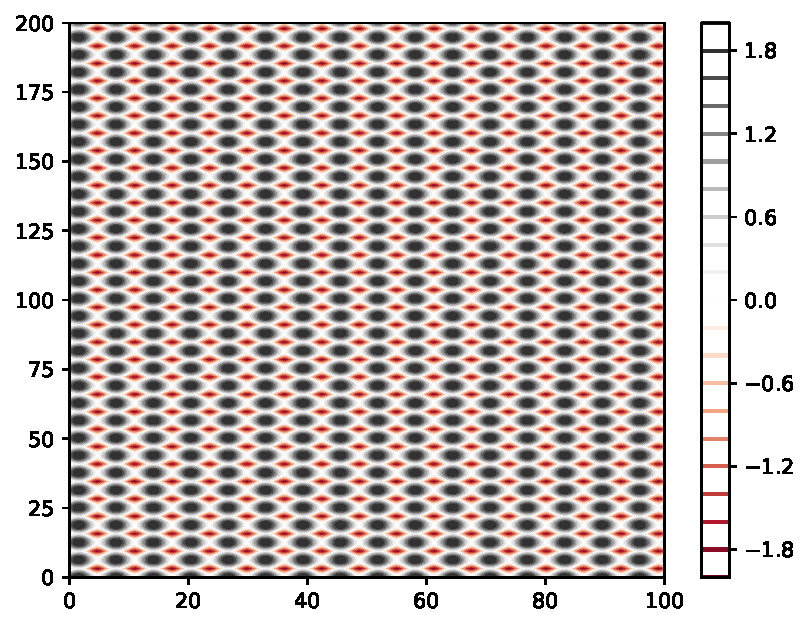
\includegraphics{guides/VisualizationPythonPackages_files/figure-pdf/cell-19-output-1.pdf}

\begin{Shaded}
\begin{Highlighting}[]
\CommentTok{\# 2D grid is interpreted as an image with imshow}
\NormalTok{plt.imshow(Z, extent}\OperatorTok{=}\NormalTok{[}\DecValTok{0}\NormalTok{, }\DecValTok{100}\NormalTok{, }\DecValTok{0}\NormalTok{, }\DecValTok{100}\NormalTok{], origin}\OperatorTok{=}\StringTok{\textquotesingle{}lower\textquotesingle{}}\NormalTok{, cmap}\OperatorTok{=}\StringTok{\textquotesingle{}RdGy\textquotesingle{}}\NormalTok{)}
\NormalTok{plt.colorbar()}
\NormalTok{plt.show()}
\end{Highlighting}
\end{Shaded}

\includegraphics{guides/VisualizationPythonPackages_files/figure-pdf/cell-20-output-1.pdf}

\begin{Shaded}
\begin{Highlighting}[]
\CommentTok{\# contour plot with labels}
\NormalTok{X }\OperatorTok{=}\NormalTok{ np.linspace(}\OperatorTok{{-}}\DecValTok{5}\NormalTok{, }\DecValTok{5}\NormalTok{, }\DecValTok{100}\NormalTok{)}
\NormalTok{Y }\OperatorTok{=}\NormalTok{ np.linspace(}\OperatorTok{{-}}\DecValTok{5}\NormalTok{, }\DecValTok{5}\NormalTok{, }\DecValTok{100}\NormalTok{)}
\NormalTok{X, Y }\OperatorTok{=}\NormalTok{ np.meshgrid(X, Y)}
\NormalTok{Z }\OperatorTok{=}\NormalTok{ np.sin(np.sqrt(X}\OperatorTok{**}\DecValTok{2} \OperatorTok{+}\NormalTok{ Y}\OperatorTok{**}\DecValTok{2}\NormalTok{))}

\NormalTok{contours }\OperatorTok{=}\NormalTok{ plt.contour(X,Y,Z,}\DecValTok{3}\NormalTok{, colors}\OperatorTok{=}\StringTok{\textquotesingle{}black\textquotesingle{}}\NormalTok{) }\CommentTok{\# plt.contour([X,Y],Z,[levels])}
\NormalTok{plt.clabel(contours, inline}\OperatorTok{=}\VariableTok{True}\NormalTok{, fontsize}\OperatorTok{=}\DecValTok{6}\NormalTok{)}
\end{Highlighting}
\end{Shaded}

\includegraphics{guides/VisualizationPythonPackages_files/figure-pdf/cell-21-output-1.pdf}

\subsection*{Seaborn}\label{seaborn}
\addcontentsline{toc}{subsection}{Seaborn}

\markright{Seaborn}

\texttt{Searborn} is based on \texttt{Matplotlib}and is made for
statistical graphics. It is comparable with \texttt{R}'s
\texttt{ggplot2} library.

It works best with \texttt{Pandas} DataFrames. You can easly create
complex plots with only a few lines of code by grouping and aggregating
data.

More informations can be found under \url{https://seaborn.pydata.org/}

\begin{Shaded}
\begin{Highlighting}[]
\ImportTok{import}\NormalTok{ seaborn }\ImportTok{as}\NormalTok{ sns}
\end{Highlighting}
\end{Shaded}

\subsubsection*{Example}\label{example}
\addcontentsline{toc}{subsubsection}{Example}

\begin{Shaded}
\begin{Highlighting}[]
\CommentTok{\# Use the default data set from seaborn}
\NormalTok{tips }\OperatorTok{=}\NormalTok{ sns.load\_dataset(}\StringTok{\textquotesingle{}tips\textquotesingle{}}\NormalTok{)}
\CommentTok{\# Create a boxplot}
\NormalTok{sns.boxplot(x}\OperatorTok{=}\StringTok{\textquotesingle{}day\textquotesingle{}}\NormalTok{, y}\OperatorTok{=}\StringTok{\textquotesingle{}total\_bill\textquotesingle{}}\NormalTok{, data}\OperatorTok{=}\NormalTok{tips)}
\end{Highlighting}
\end{Shaded}

\includegraphics{guides/VisualizationPythonPackages_files/figure-pdf/cell-23-output-1.pdf}

\begin{Shaded}
\begin{Highlighting}[]
\ImportTok{import}\NormalTok{ matplotlib.pyplot }\ImportTok{as}\NormalTok{ plt}
\ImportTok{import}\NormalTok{ seaborn }\ImportTok{as}\NormalTok{ sns}


\NormalTok{sns.set\_theme(style}\OperatorTok{=}\StringTok{"darkgrid"}\NormalTok{)}
\NormalTok{iris }\OperatorTok{=}\NormalTok{ sns.load\_dataset(}\StringTok{"iris"}\NormalTok{)}

\CommentTok{\# Set up the figure}
\NormalTok{f, ax }\OperatorTok{=}\NormalTok{ plt.subplots(figsize}\OperatorTok{=}\NormalTok{(}\DecValTok{8}\NormalTok{, }\DecValTok{8}\NormalTok{))}
\NormalTok{ax.set\_aspect(}\StringTok{"equal"}\NormalTok{)}

\CommentTok{\# Draw a contour plot to represent each bivariate density}
\NormalTok{sns.kdeplot(}
\NormalTok{    data}\OperatorTok{=}\NormalTok{iris.query(}\StringTok{"species != \textquotesingle{}versicolor\textquotesingle{}"}\NormalTok{),}
\NormalTok{    x}\OperatorTok{=}\StringTok{"sepal\_width"}\NormalTok{,}
\NormalTok{    y}\OperatorTok{=}\StringTok{"sepal\_length"}\NormalTok{,}
\NormalTok{    hue}\OperatorTok{=}\StringTok{"species"}\NormalTok{,}
\NormalTok{    thresh}\OperatorTok{=}\FloatTok{.1}\NormalTok{,}
\NormalTok{)}
\end{Highlighting}
\end{Shaded}

\includegraphics{guides/VisualizationPythonPackages_files/figure-pdf/cell-24-output-1.pdf}

\subsection*{3D plots}\label{d-plots}
\addcontentsline{toc}{subsection}{3D plots}

\markright{3D plots}

Matplotlib can also be used to create 3D plots but it is not the best
tool for this.

\begin{Shaded}
\begin{Highlighting}[]
\ImportTok{from}\NormalTok{ mpl\_toolkits.mplot3d }\ImportTok{import}\NormalTok{ Axes3D}
\ImportTok{import}\NormalTok{ matplotlib.pyplot }\ImportTok{as}\NormalTok{ plt}
\ImportTok{import}\NormalTok{ numpy }\ImportTok{as}\NormalTok{ np}

\NormalTok{fig }\OperatorTok{=}\NormalTok{ plt.figure(figsize}\OperatorTok{=}\NormalTok{(}\DecValTok{5}\NormalTok{, }\DecValTok{5}\NormalTok{))}
\NormalTok{ax }\OperatorTok{=}\NormalTok{ fig.add\_subplot(}\DecValTok{111}\NormalTok{, projection}\OperatorTok{=}\StringTok{\textquotesingle{}3d\textquotesingle{}}\NormalTok{)}
\NormalTok{x }\OperatorTok{=}\NormalTok{ np.random.standard\_normal(}\DecValTok{100}\NormalTok{)}
\NormalTok{y }\OperatorTok{=}\NormalTok{ np.random.standard\_normal(}\DecValTok{100}\NormalTok{)}
\NormalTok{z }\OperatorTok{=}\NormalTok{ np.random.standard\_normal(}\DecValTok{100}\NormalTok{)}
\NormalTok{ax.scatter(x, y, z, c}\OperatorTok{=}\StringTok{\textquotesingle{}r\textquotesingle{}}\NormalTok{, marker}\OperatorTok{=}\StringTok{\textquotesingle{}o\textquotesingle{}}\NormalTok{)}
\NormalTok{ax.set\_xlabel(}\StringTok{\textquotesingle{}X Label\textquotesingle{}}\NormalTok{)}
\NormalTok{ax.set\_ylabel(}\StringTok{\textquotesingle{}Y Label\textquotesingle{}}\NormalTok{)}
\NormalTok{ax.set\_zlabel(}\StringTok{\textquotesingle{}Z Label\textquotesingle{}}\NormalTok{)}
\NormalTok{plt.tight\_layout() }\CommentTok{\# adjust the plot to the figure}
\NormalTok{plt.show()}
\end{Highlighting}
\end{Shaded}

\includegraphics{guides/VisualizationPythonPackages_files/figure-pdf/cell-25-output-1.pdf}

Better tools for 3D plots are \texttt{Mayavi} and \texttt{Plotly}.

\subsection*{Other plotting libraries}\label{other-plotting-libraries}
\addcontentsline{toc}{subsection}{Other plotting libraries}

\markright{Other plotting libraries}

\begin{itemize}
\tightlist
\item
  \href{https://plotly.com/python/}{Plotly}
\item
  \href{https://docs.enthought.com/mayavi/mayavi/}{Mayavi}
\item
  \href{https://docs.bokeh.org/en/latest/index.html}{Bokeh}
\item
  \href{https://altair-viz.github.io/}{Altair}
\item
  \href{http://yhat.github.io/ggpy/}{ggplot}
\item
  \href{http://www.pygal.org/en/stable/}{pygal}
\item
  \href{https://pandas.pydata.org/docs/user_guide/visualization.html}{pandas}
\end{itemize}




\end{document}
